\documentclass{article}
\usepackage{graphicx} % Required for inserting images
\usepackage[a4paper, margin=1in]{geometry} % Adjust margins here
\usepackage{fancyhdr} % Required for custom headers and footers
\usepackage[backend=biber, style=ieee]{biblatex}
\usepackage{multirow}
\usepackage[normalem]{ulem}
\usepackage{tabularx}
\usepackage{array}
\usepackage{placeins}
\usepackage{xcolor}
\usepackage{longtable}
\usepackage{float}
\usepackage{listings}
\usepackage{subcaption}
\usepackage[toc,page]{appendix}

\lstdefinelanguage{json}{
    basicstyle=\ttfamily\small,
    numbers=left,
    numberstyle=\tiny\color{gray},
    stepnumber=1,
    numbersep=5pt,
    showstringspaces=false,
    breaklines=true,
    frame=single,
    backgroundcolor=\color{white},
    literate=
     *{0}{{{\color{blue}0}}}{1}
      {1}{{{\color{blue}1}}}{1}
      {2}{{{\color{blue}2}}}{1}
      {3}{{{\color{blue}3}}}{1}
      {4}{{{\color{blue}4}}}{1}
      {5}{{{\color{blue}5}}}{1}
      {6}{{{\color{blue}6}}}{1}
      {7}{{{\color{blue}7}}}{1}
      {8}{{{\color{blue}8}}}{1}
      {9}{{{\color{blue}9}}}{1}
      {:}{{{\color{red}:}}}{1}
      {,}{{{\color{red},}}}{1}
      {"}{{{\color{black}"}}}{1},
}

\lstset{
  basicstyle=\ttfamily\small,
  breaklines=true,
  frame=single,
  backgroundcolor=\color{gray!10},
  captionpos=b,
  numbers=none,
  xleftmargin=0.5cm,
  xrightmargin=0.5cm
}

\definecolor{lightgray}{rgb}{.9,.9,.9}
\definecolor{darkgray}{rgb}{.4,.4,.4}
\definecolor{purple}{rgb}{0.65, 0.12, 0.82}

\lstdefinelanguage{JavaScript}{
  keywords={typeof, new, true, false, catch, function, return, null, catch, switch, var, if, in, while, do, else, case, break},
  keywordstyle=\color{blue}\bfseries,
  ndkeywords={class, export, boolean, throw, implements, import, this},
  ndkeywordstyle=\color{darkgray}\bfseries,
  identifierstyle=\color{black},
  sensitive=false,
  comment=[l]{//},
  morecomment=[s]{/*}{*/},
  commentstyle=\color{purple}\ttfamily,
  stringstyle=\color{red}\ttfamily,
  morestring=[b]',
  morestring=[b]"
}

\lstset{
   language=JavaScript,
   backgroundcolor=\color{lightgray},
   extendedchars=true,
   basicstyle=\footnotesize\ttfamily,
   showstringspaces=false,
   showspaces=false,
   numbers=left,
   numberstyle=\footnotesize,
   numbersep=9pt,
   tabsize=2,
   breaklines=true,
   showtabs=false,
   captionpos=b
}

\lstdefinestyle{mystyle}{
    backgroundcolor=\color{gray!10},   
    commentstyle=\color{green!50!black},
    keywordstyle=\color{blue},
    numberstyle=\tiny\color{gray},
    stringstyle=\color{red},
    basicstyle=\ttfamily\footnotesize,
    breakatwhitespace=false,         
    breaklines=true,                 
    captionpos=b,                    
    keepspaces=true,                 
    numbers=left,                    
    numbersep=5pt,                  
    showspaces=false,                
    showstringspaces=false,
    showtabs=false,                  
    tabsize=2
}
\lstset{style=mystyle}
\newcolumntype{C}[1]{>{\centering\arraybackslash}p{#1}}
\newcolumntype{M}[1]{>{\centering\arraybackslash}m{#1}}
\addbibresource{references.bib}


% Set up the fancyhdr package
\pagestyle{fancy}
\fancyhf{} % Clear all header and footer fields
\fancyhead[L]{\rule{\linewidth}{0.4pt}} % Top line
\fancyfoot[C]{\thepage} % Page number in the center of the footer

\title{%
    ELECTRONICS AND COMPUTER SCIENCE \\ 
    FACULTY OF ENGINEERING AND PHYSICAL SCIENCES \\ 
    UNIVERSITY OF SOUTHAMPTON \\ 
    \vspace{1em} % Adds vertical space between title and subtitle
    \textbf{Enhancing Hearing Health: A User-Centric Application for Hearing Aid Services}%
}
\author{Nima Golshahi \\ Project Supervisor: Dr Reza Rezazadeh}
\date{29th April 2025}

\begin{document}

\fancyhead[L]{} 
\fancyhead[L]{\textbf{1 Introduction} \vspace{1pt}} % "CONTENTS" title

\section{Introduction}
\subsection{Problem}
Many older adults are reluctant to wear hearing aids because of concerns about their appearance or because they are overwhelmed by the purchasing process. Research shows that more than 80\% of people who could benefit from hearing aids do not use them, with stigma and complicated device selection being major deterrents \cite{mccormack2013}. Additionally, navigating appointments for hearing-related consultations or treatments can be challenging, especially for users unfamiliar with modern digital systems. This often leads to a delay in treatment, which can have serious cognitive and social consequences \cite{slade2020}.

The problem this project addresses is twofold: \\
(1) how to encourage older adults to try hearing aids by reducing the stigma and simplifying the selection process, and (2) how to streamline the booking and consultation process to make seeking treatment more accessible.

\subsection{Goals}
The project aims to provide a comprehensive solution to the barriers older adults face when dealing with hearing aids. The specific goals of the project include \begin{itemize} \item Creating an intuitive user interface tailored to elderly users with simple navigation and assistive technology support. \item Developing an AI-driven hearing test to assess hearing abilities in real-time, with personalized feedback. \item Implementing a streamlined booking system for audiology-related services such as hearing tests, consultations, and procedures like wax removal. \item Integrating augmented reality (AR) to allow users to visualize hearing aids on themselves before making a purchase decision. \item Using AI-based sound profiling to recommend hearing aids that best suit the user’s needs. \item Providing a notification system for appointment reminders, hearing aid maintenance, and follow-up hearing tests. \item Incorporating telehealth features for virtual consultations, reducing the need for in-person appointments. \item Offering a chatbot for FAQ and live support, helping users with questions about hearing aids or audiology services. \end{itemize}

These goals aim to improve the overall experience of purchasing and managing hearing aids, reducing the barriers that currently prevent older adults from seeking help.


\subsection{In-Scope}
The project will focus on developing core features that address the identified problem. The following elements are considered in-scope: \begin{itemize} \item User Interface Design: A simple and accessible UI that includes multilingual support and compatibility with assistive technologies. \item Hearing Test: An interactive AI-driven hearing test that offers real-time feedback and personalized sound profiling. \item Appointment System: An integrated system for booking consultations, hearing tests, and other audiology services. \item Augmented Reality (AR): A feature allowing users to visualize and customize hearing aids in real time. \item Telehealth Consultations: A platform for virtual consultations with audiologists, reducing the need for in-person visits. \item Notifications: A notification system for appointments, hearing aid maintenance, and reminders for periodic hearing tests. \item Chatbot: An AI-powered chatbot providing users with support and information about hearing aids, appointments, and services. \item AI Sound Profiling: An algorithm for recommending hearing aids based on the user's sound preferences and hearing test results. \end{itemize}

\subsection{Out-Of-Scope}
Some features and functionalities fall outside the scope of this project to ensure focus on key goals: \begin{itemize} \item Hardware Development: The project will not develop any physical hardware, such as hearing aids or hearing test devices. \item Insurance Integration: There will be no integration with insurance systems or billing management within the application. \item Offline Functionality: The project will focus on online functionalities, and there will be limited support for offline access. \item Non-Audiology-Related Medical Services: The application will not address any medical services unrelated to audiology, such as general telemedicine features. \end{itemize}

\newpage
\fancyhead[L]{} 
\fancyhead[L]{\textbf{2 Literature Review} \vspace{1pt}} % "CONTENTS" title

\section{Literature Review}
This section focuses on the analysis done involving similar applications and it also has a detailed explanation of all tools and environments planned to be used during the development phase of the app.

\subsection{Background Research}
This section provides an overview of key competitors in the hearing aid industry, focusing on their online presence and services, including hearing tests and purchasing processes. The websites analyzed are Boots Hearingcare, Specsavers, Amplifon, Hidden Hearing, Outside Clinic, and GN Resound. Each offers a different experience, but none fully addresses all the needs of older adults, particularly in terms of augmented reality (AR) and seamless user experience.

\subsubsection{Boots Hearingcare}
Boots Hearingcare offers a visually appealing website, although the landing page is quite lengthy, which may be overwhelming for older users. The website does not disclose the prices of hearing aids, potentially creating uncertainty for those considering a purchase. Its online hearing test consists of a few simple questions, with a feature to check background noise using the device’s microphone. However, the test is limited to tone sounds and does not simulate real-life hearing environments. The results provided by the test lack detailed insights into the user's hearing condition.

One standout feature is the inclusion of a hearing loss simulator that demonstrates how hearing aids can improve hearing, offering a helpful visualization for potential customers. However, hearing appointments are only available in physical stores, with no mobile service, limiting accessibility for less mobile users.

\subsubsection{Specsavers}
Specsavers primarily focuses on eyewear but also offers hearing aid services. The website is simple to navigate and provides a starting price for hearing aids, which helps users gauge affordability. However, its online hearing test is similar to Boots Hearingcare's, limited to tone sounds with no real-life scenario testing. Additionally, the website does not offer a hearing loss simulator, missing an opportunity to demonstrate the benefits of hearing aids practically.

\subsubsection{Amplifon}
Amplifon provides the best online hearing test experience among the competitors, offering a more engaging and detailed assessment of hearing ability. However, the website features a long landing page, which is not particularly user-friendly, especially for older individuals. Amplifon offers a free 14-day trial of hearing aids, which is a strong advantage for users who are hesitant to commit to a purchase. Despite these positives, the user experience could be improved with a more streamlined interface.

\subsubsection{Hidden Hearing}
Hidden Hearing’s website feels crowded and difficult to navigate, which could deter potential users. The online hearing test requires personal information to access, which is not necessary for completing the test and could discourage users from proceeding. Additionally, the test itself is difficult to find on the website. On the plus side, Hidden Hearing’s test includes both tones and real-life situations, offering a more comprehensive evaluation of hearing loss. However, similar to other competitors, the prices of hearing aids are not disclosed on the website.

\subsubsection{Outside Clinic}
Outside Clinic provides a clean and easy-to-use website that avoids overwhelming users. However, it requires personal information to access the hearing test, which may be seen as a barrier for users concerned about privacy. Like many of its competitors, Outside Clinic does not disclose the prices of hearing aids on its website, and while the test is easy to find, it lacks some of the more advanced features available elsewhere.

\subsubsection{GN Resound}
GN Resound’s online hearing test is one of the weaker offerings. It simply asks users to drag a volume control until they can barely hear a sound, which is highly subjective and may not provide an accurate assessment of hearing loss. Additionally, the website does not provide pricing information for hearing aids, which is a common drawback among the competitors. The test's simplicity and lack of precision limit its usefulness for users seeking a detailed evaluation of their hearing.

\subsection{Design Considerations for Accessibility in Older Adults}

Hearing loss is prevalent among older adults, making accessibility a core component in the design of applications intended for this demographic. Effective design for older users addresses both the physical and cognitive challenges often associated with ageing, ensuring an intuitive and seamless user experience. This section explores key design principles that have been incorporated into the application to optimize usability and accessibility for elderly users.

\subsubsection{Visual Accessibility}
Older adults frequently experience reduced visual acuity \cite{vanderPols2000}, which can hinder interaction with small text and low-contrast elements. To accommodate this, the interface uses large, high-contrast fonts that enhance readability. A simple, uncluttered layout with minimal visual noise further aids in focusing attention on essential elements. Key buttons and interactive elements are highlighted with distinctive colours, and options for text resizing are available to further improve legibility.

\subsubsection{Simplified Navigation}
Cognitive load can increase with age, making simple navigation essential \cite{doube2012}. The application employs a straightforward, linear navigation structure, avoiding complex or nested menus that could overwhelm users. Clear labels and intuitive icons accompany all actions, enabling a quick understanding of available functions. Additionally, critical features such as the AR visualization of hearing aids and the hearing test are placed prominently on the landing page, reducing the need for excessive searching.

\subsubsection{Touch-Target Size and Interaction Design}
Motor control can also decline with age, making precise touch interactions challenging. The app incorporates large touch-target areas for all buttons and interactive elements, minimizing the risk of accidental mis-taps. Furthermore, the app limits the need for complex gestures, such as swiping, and instead uses simple tap-and-hold interactions where necessary \cite{CASTILLA2016909}.

\subsection{Tools and Environment}
This subsection outlines the tools and environments used in the development of the hearing aid web application and its Progressive Web App (PWA) version. The choices are motivated by the need for cross-platform compatibility, efficient project management, and a streamlined design-to-development workflow that optimizes the user experience for older adults.

\subsubsection{Design Tool: Figma}
Figma will be used for designing both the web and PWA interfaces. Figma offers an intuitive, collaborative environment, allowing real-time feedback on wireframes and prototypes. Its cloud-based nature supports seamless handoff between the design and development phases, which is essential for refining the user interface for older adults, who are the primary audience of this application.

\subsubsection{Hosting Infrastructure: Azure Web App}
Azure Web App is chosen for hosting the hearing aid web application due to its fully managed nature, scalability, and seamless integration with both backend and frontend services. It supports automatic scaling, ensuring optimal performance as the number of users grows. Azure Web App also offers robust security features, such as SSL/TLS encryption, and enables easy continuous integration and deployment (CI/CD) through Azure DevOps \cite{azureappservice}. Additionally, the Azure Web App integrates well with Azure OpenAI, enabling efficient AI-driven features like the hearing test and personalized recommendations. This makes Azure Web App an ideal solution for hosting the web and PWA, providing a reliable, secure, and scalable environment.

\subsubsection{Programming Language: JavaScript and Kotlin}
JavaScript will be used for developing the web application and PWA, enabling dynamic, responsive behaviour. JavaScript's extensive ecosystem supports integrating features like AR and interactive components. Additionally, Kotlin will be used on the backend for API development, maintaining a consistent language across the stack and facilitating code sharing for potential mobile expansion.

\subsubsection{Web Development Framework: React}
React will be used for building the front end of both the web app and PWA. As a fast, component-based library, React allows for the creation of a responsive and accessible user interface. It also integrates well with modern JavaScript frameworks and libraries, making it an ideal choice for efficiently developing interactive web pages and progressive web app features.

\subsubsection{Service Worker and Offline Support: Workbox}
Workbox, a tool developed by Google, will manage service worker setup for the PWA. It simplifies caching strategies, offline support, and background syncing. By using Workbox, the application can provide an offline experience and background updates, essential for ensuring older users have uninterrupted access to information, even without constant internet connectivity.

\subsubsection{Backend Framework: Ktor}
Ktor will be used for developing the backend APIs, allowing the project to stay within a Kotlin-based backend framework. Ktor is lightweight and flexible, making it suitable for managing server-side logic such as handling user profiles, appointment scheduling, and hearing test data. This approach supports a RESTful API structure compatible with both web and PWA frontend requirements.

\subsubsection{Development Environment: IntelliJ IDEA}
IntelliJ IDEA will be used as the primary development environment. It provides extensive support for Kotlin and integrates well with web technologies like React, making it suitable for both backend and frontend development. IntelliJ facilitates efficient debugging, code navigation, and plugin support, which are valuable for a seamless development workflow across the project.

\subsubsection{Database: Firebase and CosmosDB}
Firebase will handle real-time data storage, particularly for lightweight, real-time interactions in the PWA. For larger datasets, Azure Cosmos DB will manage user profiles, hearing test results, and appointment data. CosmosDB’s globally distributed storage offers low-latency performance, which is ideal for handling user interactions on a large scale.

\subsubsection{Version Control: GitHub}
Version control will be managed through GitHub, allowing for efficient tracking of code changes, branch management, and collaboration across the development team. GitHub will store both the frontend React code and the Kotlin-based backend, ensuring a unified repository for managing the project.

\subsubsection{Project Management: ClickUp}
ClickUp will be used for organizing tasks, tracking progress, and managing deadlines. Its task management, time tracking, and collaboration features help keep the project on schedule, providing transparency and accountability for each phase of the development cycle.

\subsubsection{Diagram Creation: LucidChart}
Lucidchart will be used to create system architecture diagrams, flowcharts, and UML diagrams, which are essential for visualizing data flow and backend architecture. This helps ensure alignment between backend processes and frontend interfaces, particularly when handling data interactions and user interface elements.


\newpage

\fancyhead[L]{} 
\fancyhead[L]{\textbf{3 System Analysis} \vspace{1pt}} % "CONTENTS" title

\section{System Analysis}

This section focuses on the system analysis of the application which involves the identification of Stakeholders, User Stories, Functional and Non-Functional Requirements and Risk Analysis. 

\subsection{Stakeholder Analysis}

Stakeholder analysis should be conducted before the project (actual coding)
is initiated. Its main purpose is to help me as the developer identify all categories of individuals involved in the application. Furthermore, will be possible
to prioritize these people as primary, secondary and facilitating stakeholders
always according to their influence on the project. Primary stakeholders are
the ones that directly interact with the application whereas, secondary stakeholders do not directly interact with the system but have a reasonable influence
on it. Tertiary stakeholders are the ones that are only affected by the system. Concluding, facilitating stakeholders are the ones that are involved in
developing and maintaining the system. \cite{termscompared2019}

\begin{table}[h]
    \centering
    \vspace{10pt}
    \begin{tabular}{|l|l|p{9cm}|}
        \hline
        \textbf{Stakeholder} & \textbf{Type} & \textbf{Role/Description} \\ \hline
        End Users & Primary & Older individuals seeking hearing aids and related services, focusing on usability and minimizing stigma. \\ \hline
        Audiologists & Primary & Professionals provide consultations, manage appointments, and offer feedback on hearing tests and device recommendations. \\ \hline
        Family Members/Caregivers & Secondary & Assist users in navigating the app, requiring an intuitive design for easy management of user settings. \\ \hline
        Hearing Aid Manufacturers & Secondary & Potential partners provide product information, enabling informed choices for users. \\ \hline
        Nima Golshahi & Internal & Sole developer is responsible for the design, development, and maintenance of the application. \\ \hline
        Healthcare Providers & Secondary & Clinics or hospitals may refer patients to the app for preliminary assessments or services. \\ \hline
    \end{tabular}
    \label{tab:stakeholder_analysis}
    \caption{Stakeholder Analysis}
\end{table}

The table above identifies each stakeholder involved in the Hearing Health app according to his/ her type.

\subsection{User Stories}
By having user stories it is possible to capture high-level requirements. The
main template of a user story is: As a “persona” I want to “action”,
so that I “receive benefit”. This helps me as the developer to get a better
understanding of the precise user requirements so that I can stay focused on the end user’s needs. \cite{airfocus2024}
The tables below describe the User Stories of my primary stakeholders who directly interact with my application. A
user story always has a number (id) and a priority. The MoSCoW prioritisation will be used which represents 5 categories of initiatives: must-have,
should-have, could-have, and won’t-have, or will not have right now \cite{productplan2024}. This
will help me as a developer manage my project more effectively since I will be allocating all tasks according to their priority.

\begin{table}[t]
    \centering
    \vspace{10pt}
    \begin{tabular}{|c|c|C{4cm}|c|C{4cm}|C{2cm}|}
        \hline
        \textbf{ID} & \textbf{Role}               & \textbf{Goal}                                     & \multirow{5}{*}{\textbf{So that}} & \textbf{Benefit}                                          & \textbf{MoSCoW Priority} \\ \cline{1-3} \cline{5-6} 
        US01       & \multirow{14}{*}{As a user} & View a range of hearing aids with prices and feature                      &                   & I can compare options and make an informed choice         & \textcolor{red}{Must Have}              \\ \cline{1-1} \cline{3-3} \cline{5-6} 
        US02       &                   & Select a hearing aid and try it on in AR with different colours &                   & I can see how each hearing aid would look on me & \textcolor{red}{Must Have}               \\ \cline{1-1} \cline{3-3} \cline{5-6} 
        US03       &                   & Book a consultation, fitting, micro-suction, aftercare/repair appointment                  &                   & I can receive services tailored to my needs             & \textcolor{red}{Must Have}            \\ \cline{1-1} \cline{3-3} \cline{5-6} 
        US04       &                   & Take an AI-driven hearing test        &                   &  I can assess my hearing levels accurately               & \textcolor{red}{Must Have} \\ \cline{1-1} \cline{3-3} \cline{5-6}
        US05      &                   & Contact the business      &                   &  I can reach out if I have questions or need assistance               & \textcolor{red}{Must Have} \\ \cline{1-1} \cline{3-3} \cline{5-6}
        US06       &                   & Take a quiz to determine the best type of appointment for me        &                   & I can identify which service will be most helpful                 & \textcolor{orange}{Should Have}   \\ \cline{1-1} \cline{3-3} \cline{5-6}
        US07       &                   & Take a quiz to find the most suitable type of hearing aid        &                   &  I can discover the hearing aid model that fits my needs                & \textcolor{orange}{Should Have} \\ \cline{1-1} \cline{3-3} \cline{5-6}
        US08       &                   & Pay for appointments via various methods      &                   &  I can choose a convenient payment option               & \textcolor{orange}{Should Have} \\ \cline{1-1} \cline{3-3} \cline{5-6}
        US09       &                   & Create and manage my user profile, view upcoming appointments, and leave feedback      &                   &  I can have control over my appointments and provide feedback               & \textcolor{green}{Could Have} \\ \cline{1-1} \cline{3-3} \cline{5-6}
        US10       &                   & Receive notifications for updates like hearing aid arrival time and upcoming appointments      &                   &   I am aware of important updates               & \textcolor{green}{Could Have} \\ \cline{1-1} \cline{3-3} \cline{5-6}
        US11       &                   & Find nearby audiologists based on my location      &                   &  I can conveniently find a provider near me               & \textcolor{green}{Could Have} \\ \cline{1-1} \cline{3-3} \cline{5-6}
        US12       &                   & Save my favorite audiologists for easy booking     &                   &  I can quickly rebook with someone I trust               & \textcolor{blue}{Won't Have} \\ \cline{1-1} \cline{3-3} \cline{5-6}
        US13       &                   & View a summary of my hearing history and test results     &                   &  I can track my hearing health over time               & \textcolor{blue}{Won't Have} \\ \cline{1-1} \cline{3-3} \cline{5-6}
        US14       &                   & Access a virtual assistant for quick questions about hearing care     &                   &  I can receive instant help without waiting for support               & \textcolor{blue}{Won't Have} \\ \hline
    \end{tabular}
    \caption{User Stories for End User}
\end{table}
\newpage
\begin{table}[t]
    \centering
    \vspace{10pt}
    \begin{tabular}{|c|c|C{4cm}|c|C{4cm}|C{2cm}|}
        \hline
        \textbf{ID} & \textbf{Role}               & \textbf{Goal}                                     & \multirow{5}{*}{\textbf{So that}} & \textbf{Benefit}                                          & \textbf{MoSCoW Priority} \\ \cline{1-3} \cline{5-6} 
        US15       & \multirow{4}{*}{As an audiologist}      & Update and manage my appointment schedule within the app        &                   & Patients can book available slots directly without needing to call             & \textcolor{red}{Must Have}               \\ \cline{1-1} \cline{3-3} \cline{5-6} 
        US16       &       & Create and manage my profile with bio, image, and upcoming/previous appointments        &                   & I can give patients a sense of my expertise             & \textcolor{red}{Must Have}               \\ \cline{1-1} \cline{3-3} \cline{5-6} 
         US17       &       & Set availability for different types of appointments        &                   & Patients can see available slots when booking appointments             & \textcolor{orange}{Should Have}               \\ \cline{1-1} \cline{3-3} \cline{5-6} 
         US18       &       & Specify the types of appointments I can perform        &                   & My schedule reflects the services I offer             & \textcolor{green}{Could Have}               \\ \cline{1-1} \cline{3-3} \cline{5-6}
         
         US19       &                   & Receive notifications for upcoming appointments        &                   & I am prepared for each consultation and can review the patient's records in advance             & \textcolor{green}{Could Have}               \\ \cline{1-1} \cline{3-3} \cline{5-6} 
         US20       &  & View a patient's hearing test results                      &                   & I can assess their hearing profile and provide informed recommendations        & \textcolor{green}{Could Have}              \\ \cline{1-1} \cline{3-3} \cline{5-6}
         US21       &       & Indicate my familiarity with certain hearing aid brands        &                   & Patients know my expertise with different brands             & \textcolor{blue}{Won't Have}               \\ \cline{1-1} \cline{3-3} \cline{5-6} 
        US22       &                   & Track patient progress and compliance with recommended hearing aid use       &                   & I can provide follow-up advice or adjustments if necessary
             & \textcolor{blue}{Won't Have}               \\ \hline
        
    \end{tabular}
    \caption{User Stories for Audiologist}
\end{table}
        

\FloatBarrier

\subsection{Functional and Non-Functional Requirements}
Functional Requirements (FRs) are a “description of the service that the software must offer”, while non-functional requirements (NFRs) are “constraints or restrictions on the design of the system”. Using the previously outlined user stories, the functional requirements of the application will be created to represent what the primary stakeholders expect from the app. This approach also helps me, as the developer, to gain a clearer understanding of stakeholder needs, guiding both the essential elements to include and the aspects to avoid during the development of the Hearing Aid Visualizer and Hearing Test App. The following sections outline the functional and non-functional requirements for the application I will develop.

\begin{table}[h]
    \centering
    \begin{tabularx}{\textwidth}{|c|c|X|}
        \hline
        \textbf{FR ID} & \textbf{US ID} & \textbf{Description} \\
        \hline
        FR01 & US01, US02 & The system must display a range of hearing aids, along with prices and features. \\
        \hline
        FR02 & US02 & The system must support Augmented Reality (AR) functionality for users to try on different hearing aids with various colour options. \\
        \hline
        FR03 & US03 & The system must allow users to book appointments, including consultation, fitting, micro-suction, and aftercare services. \\
        \hline
        FR04 & US04 & The system must provide users with an AI-driven hearing test to assess their hearing levels. \\
        \hline
        FR05 & US05 & The system must allow users to contact the business for inquiries and support. \\
        \hline
        FR06 & US06, US07 & The system must provide quizzes to help users determine the most suitable appointment or hearing aid based on their needs. \\
        \hline
        FR07 & US08 & The system must support various payment methods for appointment bookings. \\
        \hline
        FR08 & US09 & The system must allow users to create and manage their profiles, view upcoming appointments, and leave feedback. \\
        \hline
        FR09 & US10 & The system must send notifications to users about important updates like hearing aid arrival time and upcoming appointments. \\
        \hline
        FR10 & US11 & The system must enable users to find nearby audiologists based on their location. \\
        \hline
        FR11 & US12 & The system must allow users to save their favourite audiologists for easy future bookings. \\
        \hline
        FR12 & US13 & The system must provide users with a summary of their hearing test results and history. \\
        \hline
        FR13 & US14 & The system must include a virtual assistant for quick queries about hearing care. \\
        \hline
        FR14 & US15 & Audiologists must be able to manage and update their appointment schedules within the system. \\
        \hline
        FR15 & US16 & Audiologists must be able to create and manage their profiles, including bio, images, and appointment history. \\
        \hline
        FR16 & US17 & Audiologists must be able to set their availability for different types of appointments. \\
        \hline
        FR17 & US18 & Audiologists must specify the types of appointments they are available to perform. \\
        \hline
        FR18 & US19 & Audiologists must receive notifications for upcoming appointments. \\
        \hline
        FR19 & US20 & Audiologists must be able to view a patient's hearing test results to assess their hearing profile. \\
        \hline
        FR20 & US21 &  Audiologists must indicate their familiarity with various hearing aid brands to inform patients of their expertise.\\
        \hline
        FR21 & US22 & Audiologists must track a patient's progress and compliance with hearing aid use for follow-up consultations. \\
        \hline
    \end{tabularx}
    \caption{Functional Requirements}
\end{table}

\newpage

\begin{table}[h]
    \centering
    \begin{tabularx}{\textwidth}{|c|X|}
        \hline
        \textbf{NFR ID} & \textbf{Description} \\
        \hline
        NFR01 & The system must be available 24/7 with minimal downtime for maintenance or updates. \\
        \hline
        NFR02 & The system must support high availability and handle a large number of concurrent users. \\
        \hline
        NFR03 & The system must load within 3 seconds to ensure a responsive and smooth user experience. \\
        \hline
        NFR04 & The system must provide secure data encryption, especially for user profiles, payment details, and hearing test results. \\
        \hline
        NFR05 & The system must comply with relevant privacy regulations (such as GDPR or HIPAA) for user data. \\
        \hline
        NFR06 & The system must be user-friendly, with an intuitive interface for users and audiologists. \\
        \hline
        NFR07 & The system must support a wide range of devices, including smartphones, tablets, and desktops, for both users and audiologists. \\
        \hline
        NFR08 & The system must be scalable to accommodate future feature additions or increased user load. \\
        \hline
        NFR09 & The system must provide real-time notifications to users and audiologists with a maximum delay of 5 minutes. \\
        \hline
        NFR10 & The system must support multiple languages, including English, Spanish, and other relevant languages for accessibility. \\
        \hline
        NFR11 & The system must provide accessibility features, including support for screen readers and high-contrast mode. \\
        \hline
    \end{tabularx}
    \caption{Non-Functional Requirements}
\end{table}

\subsection{Requirements Elicitation}
Requirements elicitation is the process of identifying the functionalities and constraints of the application to ensure it meets user needs and expectations. For this project, the requirements were gathered primarily through the following two methods: analysis of competitor websites and insights from my parents, who are audiologists with extensive experience in the field. These approaches provided a comprehensive understanding of the needs for the application.

\subsubsection{Competitor Analysis} An important part of the requirements elicitation process involved examining existing websites and services provided by competitors in the audiology and hearing aid sector. Key competitors such as Boots Hearingcare, Specsavers, Amplifon, and Hidden Hearing were analyzed. Although these companies provide a range of services, none of them currently offer Augmented Reality (AR) functionality for virtual try-ons of hearing aids. This gap in the market presents an opportunity for the application to differentiate itself by incorporating AR features, which could help users visualize hearing aids in a realistic setting before making a purchase.

Additionally, the analysis revealed common features across competitor websites, such as appointment booking tools, access to hearing test results, and detailed information about hearing aids. These insights formed the basis for similar functionalities in the application, ensuring that the app meets the current industry standards while offering an innovative twist with AR.

\subsubsection{Audiologist Insights} I also sought advice from my parents, who are both experienced audiologists, to ensure that the application aligns with professional practices and addresses real-world user needs. Their feedback emphasized the importance of the following features: 
\begin{itemize} 
    \item \textbf{Ease of Use:} Many older users, who are the target audience for this application, may have limited technical experience. Therefore, the interface needs to be user-friendly, intuitive, and simple to navigate. 
    \item \textbf{Accurate Product Information:} It is crucial that users have access to detailed information about different hearing aid models, their features, and benefits, to help them make informed decisions. 
    \item \textbf{AI-Based Hearing Tests:} An AI-driven hearing test can serve as a useful tool to help users assess whether they need to book an appointment with an audiologist. It is not intended to replace professional evaluation, but rather to offer a preliminary confirmation or alert users when further consultation with an audiologist is necessary.
    \item \textbf{Appointment Scheduling:} The app should include functionality to schedule appointments with audiologists, which is an essential service that current competitors also offer. 
\end{itemize}

\subsubsection{Documenting the Requirements} The insights gathered from the competitor analysis and feedback from audiologist professionals were synthesized into both functional and non-functional requirements. Functional requirements include features such as AR-based try-ons, AI-powered hearing tests, and appointment scheduling. Non-functional requirements include system performance, reliability, security, and scalability to ensure a smooth user experience.



\newpage

\fancyhead[L]{} 
\fancyhead[L]{\textbf{4 Project Planning} \vspace{1pt}} % "CONTENTS" title

\section{Project Planning}
This section focuses on the Product Backlog of the application. It analyzes the Agile Methods (Sprint Planning) and the Gantt Chart.
\subsection{Agile Methods}
Agile methodology is utilised in this project as a means “to transform an idea and varied needs into feasible software solutions”. More precisely, agile methodology is a collection of techniques that aids the development team in dividing the project into smaller, manageable components. This approach enables the developers to adapt to changing requirements and unexpected time constraints more effectively \cite{sarangam2021agile}.

When adopting Scrum, the first step is to create a Product Backlog, which is defined as “a prioritised list of deliverables ... that helps you estimate, refine, and prioritise everything you might at some point in the future wish to complete” \cite{karlsson_agile_backlogs}. The Product Backlog for the Hearing Care application can be found in the System Analysis section.
\subsubsection{Sprint Planning}
Once the product backlog is completed, the developers typically proceed with sprint planning. Using the product backlog, the team breaks the project plan into different sprints, with each sprint containing specific tasks and a defined time frame, usually between one week and one month, to complete them. This approach allows the team to focus on individual goals rather than the entire project \cite{adobe_workfront_sprints}.

After thoroughly analysing the user stories, functional, and non-functional requirements, the tasks needed to develop the Hearing Aid Visualisation App have been divided into three sprints. The tasks were prioritised using the MoSCoW prioritisation method to ensure that most "Must-have" features were included in the first two sprints. This ensures that, if any challenges arise during development, lower-priority tasks ("Should-have" or "Could-have") can be reprioritised or excluded.

The three sprints also incorporate ongoing research activities, as this will be conducted throughout the development phase. Below are the Sprint Backlog tables, which outline the tasks for each sprint.


\begin{table}[H]
\centering
\label{tab:functional-requirements}
\begin{tabular}{|c|p{8cm}|c|}
\hline
\textbf{FR ID} & \textbf{Description} & \textbf{MoSCoW Priority} \\ \hline
FR01 & The system must display a range of hearing aids, along with prices and features. & \textcolor{red}{Must Have} \\ \hline
FR03 & The system must allow users to book appointments, including consultation, fitting, micro-suction, and aftercare services. & \textcolor{red}{Must Have} \\ \hline
FR04 & The system must provide users with an AI-driven hearing test to assess their hearing levels. & \textcolor{red}{Must Have} \\ \hline
FR05 & The system must allow users to contact the business for inquiries and support. & \textcolor{red}{Must Have} \\ \hline
\end{tabular}
\caption{Sprint 1}
\end{table}

\begin{table}[H]
\centering
\label{tab:functional-requirements}
\begin{tabular}{|c|p{8cm}|c|}
\hline
\textbf{FR ID} & \textbf{Description} & \textbf{MoSCoW Priority} \\ \hline
FR02 & The system must support Augmented Reality (AR) functionality for users to try on different hearing aids with various colour options. & \textcolor{red}{Must Have} \\ \hline
FR14 & Audiologists must be able to manage and update their appointment schedules within the system. & \textcolor{red}{Must Have} \\ \hline
FR15 & Audiologists must be able to create and manage their profiles, including bio, images, and appointment history & \textcolor{red}{Must Have} \\ \hline
FR06 & The system must provide quizzes to help users determine the most suitable appointment or hearing aid based on their needs & \textcolor{orange}{Should Have} \\ \hline
FR07 & The system must support various payment methods for appointment bookings. & \textcolor{orange}{Should Have} \\ \hline
\end{tabular}
\caption{Sprint 2}
\end{table}

\begin{table}[H]
\centering
\label{tab:functional-requirements}
\begin{tabular}{|c|p{8cm}|c|}
\hline
\textbf{FR ID} & \textbf{Description} & \textbf{MoSCoW Priority} \\ \hline
FR16 & Audiologists must be able to set their availability for different types of appointments. & \textcolor{orange}{Should Have} \\ \hline
FR08 & The system must allow users to create and manage their profiles, view upcoming appointments, and leave feedback.  & \textcolor{green}{Could Have} \\ \hline
FR09 & The system must send notifications to users about important updates like hearing aid arrival time and upcoming appointments. & \textcolor{green}{Could Have} \\ \hline
FR17 & Audiologists must specify the types of appointments they are available to perform. & \textcolor{green}{Could Have} \\ \hline
\end{tabular}
\caption{Sprint 3}
\end{table}

\subsection{Gantt Chart}

\begin{figure}[H]
    \centering
    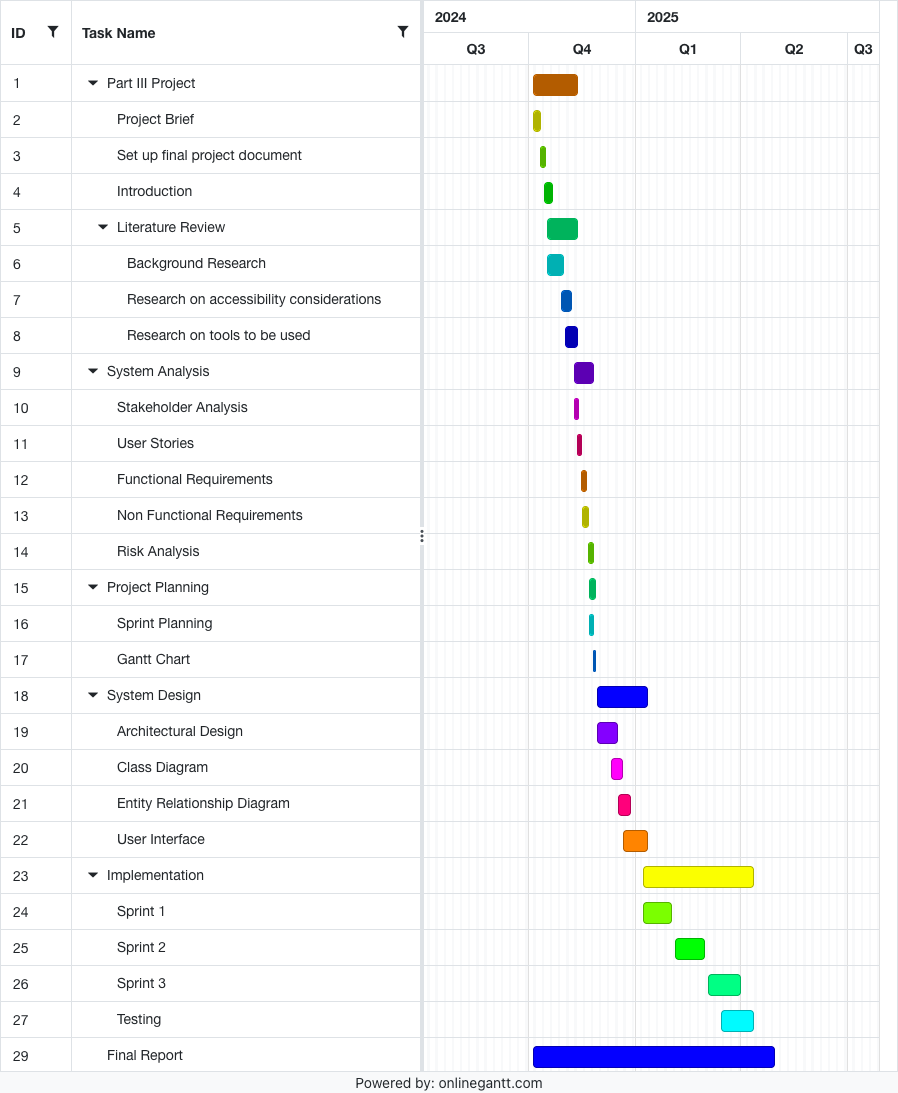
\includegraphics[width=\textwidth]{Gantt Chart.png}
    \caption{Project timeline represented in the Gantt Chart.}
    \label{fig:gantt_chart}
\end{figure}

\subsection{Risk Analysis}

\begin{table}[H]
    \centering
    \begin{tabularx}{\textwidth}{|X|c|c|c|X|}
        \hline
        \textbf{Risk} & \textbf{P} & \textbf{S} & \textbf{RE} & \textbf{Mitigation} \\
        \hline
        Lack of sufficient technical knowledge or experience in AR for hearing aid visualization. & 4 & 5 & 20 & Seek external resources, training, and tutorials. Explore existing AR frameworks. \\
        \hline
        Delays due to being the only developer and handling all tasks (design, development, testing, etc.). & 5 & 5 & 25 & Prioritize tasks, create a detailed schedule, and break down tasks into manageable chunks. \\
        \hline
        Difficulty in managing project deadlines due to personal time constraints. & 4 & 4 & 16 & Create a realistic project timeline, allocate specific time blocks for development, and track progress regularly. \\
        \hline
        Integration challenges with external APIs (e.g., payment gateways, AI-driven hearing tests). & 3 & 4 & 12 & Research APIs thoroughly, and conduct testing early. Ensure clear documentation is available and be ready for troubleshooting. \\
        \hline
        System performance issues (e.g., slow response time, high load) if scalability is not properly considered. & 3 & 5 & 15 & Optimize code and infrastructure for scalability. Implement performance testing and monitoring tools. \\
        \hline
        Bugs or issues with the mobile and web interfaces due to limited testing resources. & 4 & 3 & 12 & Perform thorough testing during development, and consider using automated testing tools. Conduct user testing to uncover potential issues. \\
        \hline
        Inadequate security measures, leading to potential data breaches (especially for sensitive user data). & 2 & 5 & 10 & Implement industry-standard security protocols (e.g., data encryption, two-factor authentication). \\
        \hline
        Compatibility issues with different devices or platforms, affecting accessibility and user experience. & 3 & 4 & 12 & Test on multiple devices and platforms. Use responsive design principles and consider a cross-platform framework for consistency. \\
        \hline
        Potential non-compliance with privacy regulations (e.g., GDPR, HIPAA) due to improper handling of user data. & 2 & 5 & 10 & Stay informed on relevant privacy regulations, and ensure proper data handling practices are followed. \\
        \hline
        Overestimation of the ability to complete the project within the given timeframe. & 4 & 4 & 16 & Set realistic expectations, frequently review project progress, and adjust timelines as necessary. \\
        \hline
        Lack of user feedback or adoption after release, reducing the app’s effectiveness. & 3 & 3 & 9 & Incorporate user feedback during development through beta testing. Use analytics tools to track user behaviour and improve the app post-launch. \\
        \hline
    \end{tabularx}
    \caption{Risk Analysis with Probability, Severity, Risk Exposure, and Mitigation}
\end{table}



\newpage

\fancyhead[L]{} 
\fancyhead[L]{\textbf{5 System Design} \vspace{1pt}} 


\section{System Design}
This section will include all system design aspects of the application. All aspects are described in the System Architecture, class diagram, Entity-Relationship diagram, Desktop user interface and mobile user interface wireframes subsections.
\subsection{System Architecture}
\begin{figure}[H]
    \centering
    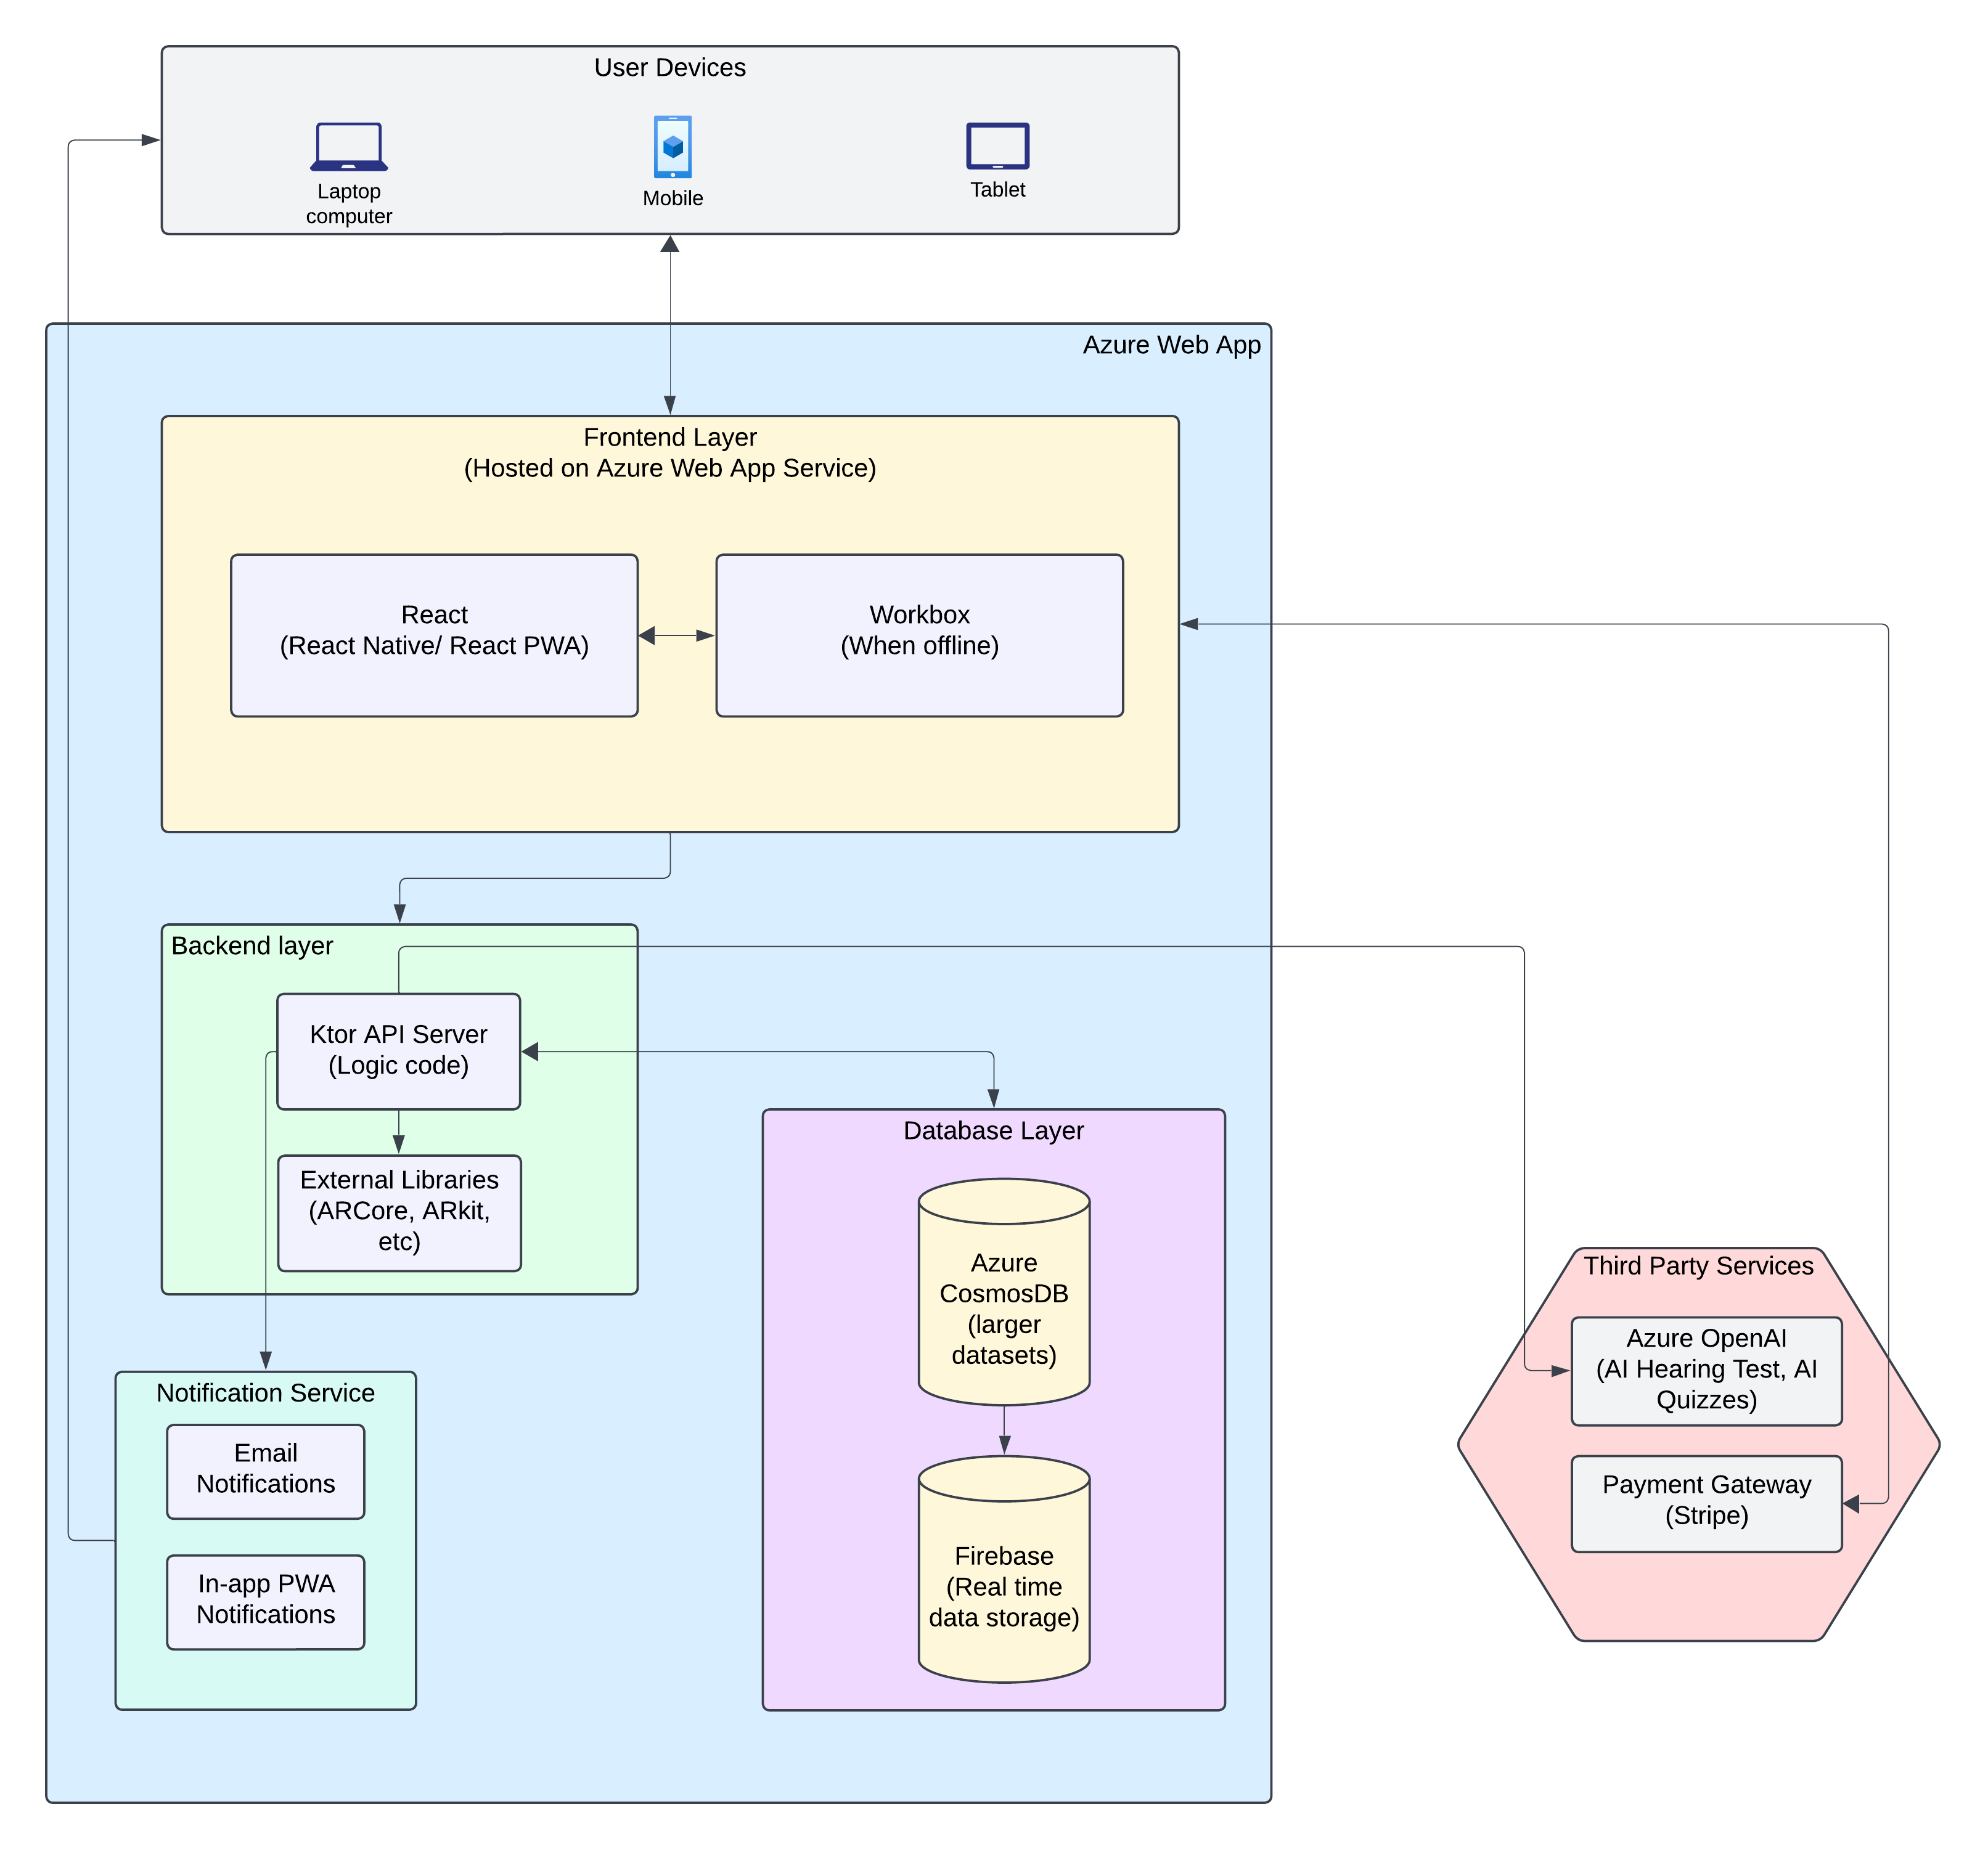
\includegraphics[width=\textwidth]{systemarchitecture.png}
    \caption{System Architecture Diagram}
    \label{fig:system-architecture}
\end{figure}

The system architecture diagram clearly shows the hierarchical relationships between various components, with each layer depending on lower-level classes or services. At the top of the diagram, the user devices (such as computers, tablets, and mobiles) interact with the Frontend Layer, which is responsible for rendering the user interface. The Frontend Layer communicates with the Backend Layer, which includes the Ktor API server. The API server, in turn, relies on external libraries and services, such as Azure OpenAI and Stripe, for specialized functionalities like AI-powered features and payment processing. The Backend Layer also interacts with the Database Layer, which combines Azure Cosmos DB for large-scale data and Firebase for real-time updates. The repository pattern is used to abstract data handling, ensuring efficient access to both persistent data and remote data sources \cite{repositoryPattern}. For smooth operation, each class and component must work seamlessly to provide the user with a responsive, reliable, and efficient experience across platforms.

\subsection{Class Diagram}
The diagram below represents all the classes, objects and methods to make an analyzed representation of the structure of the system. The class diagram will make it easier for the developer to understand and get a better visualization of all the different elements needed for the implementation along with the synergy and properties that they have \cite{wikipedia_class_diagram}. 

\begin{figure}[H]
    \centering
    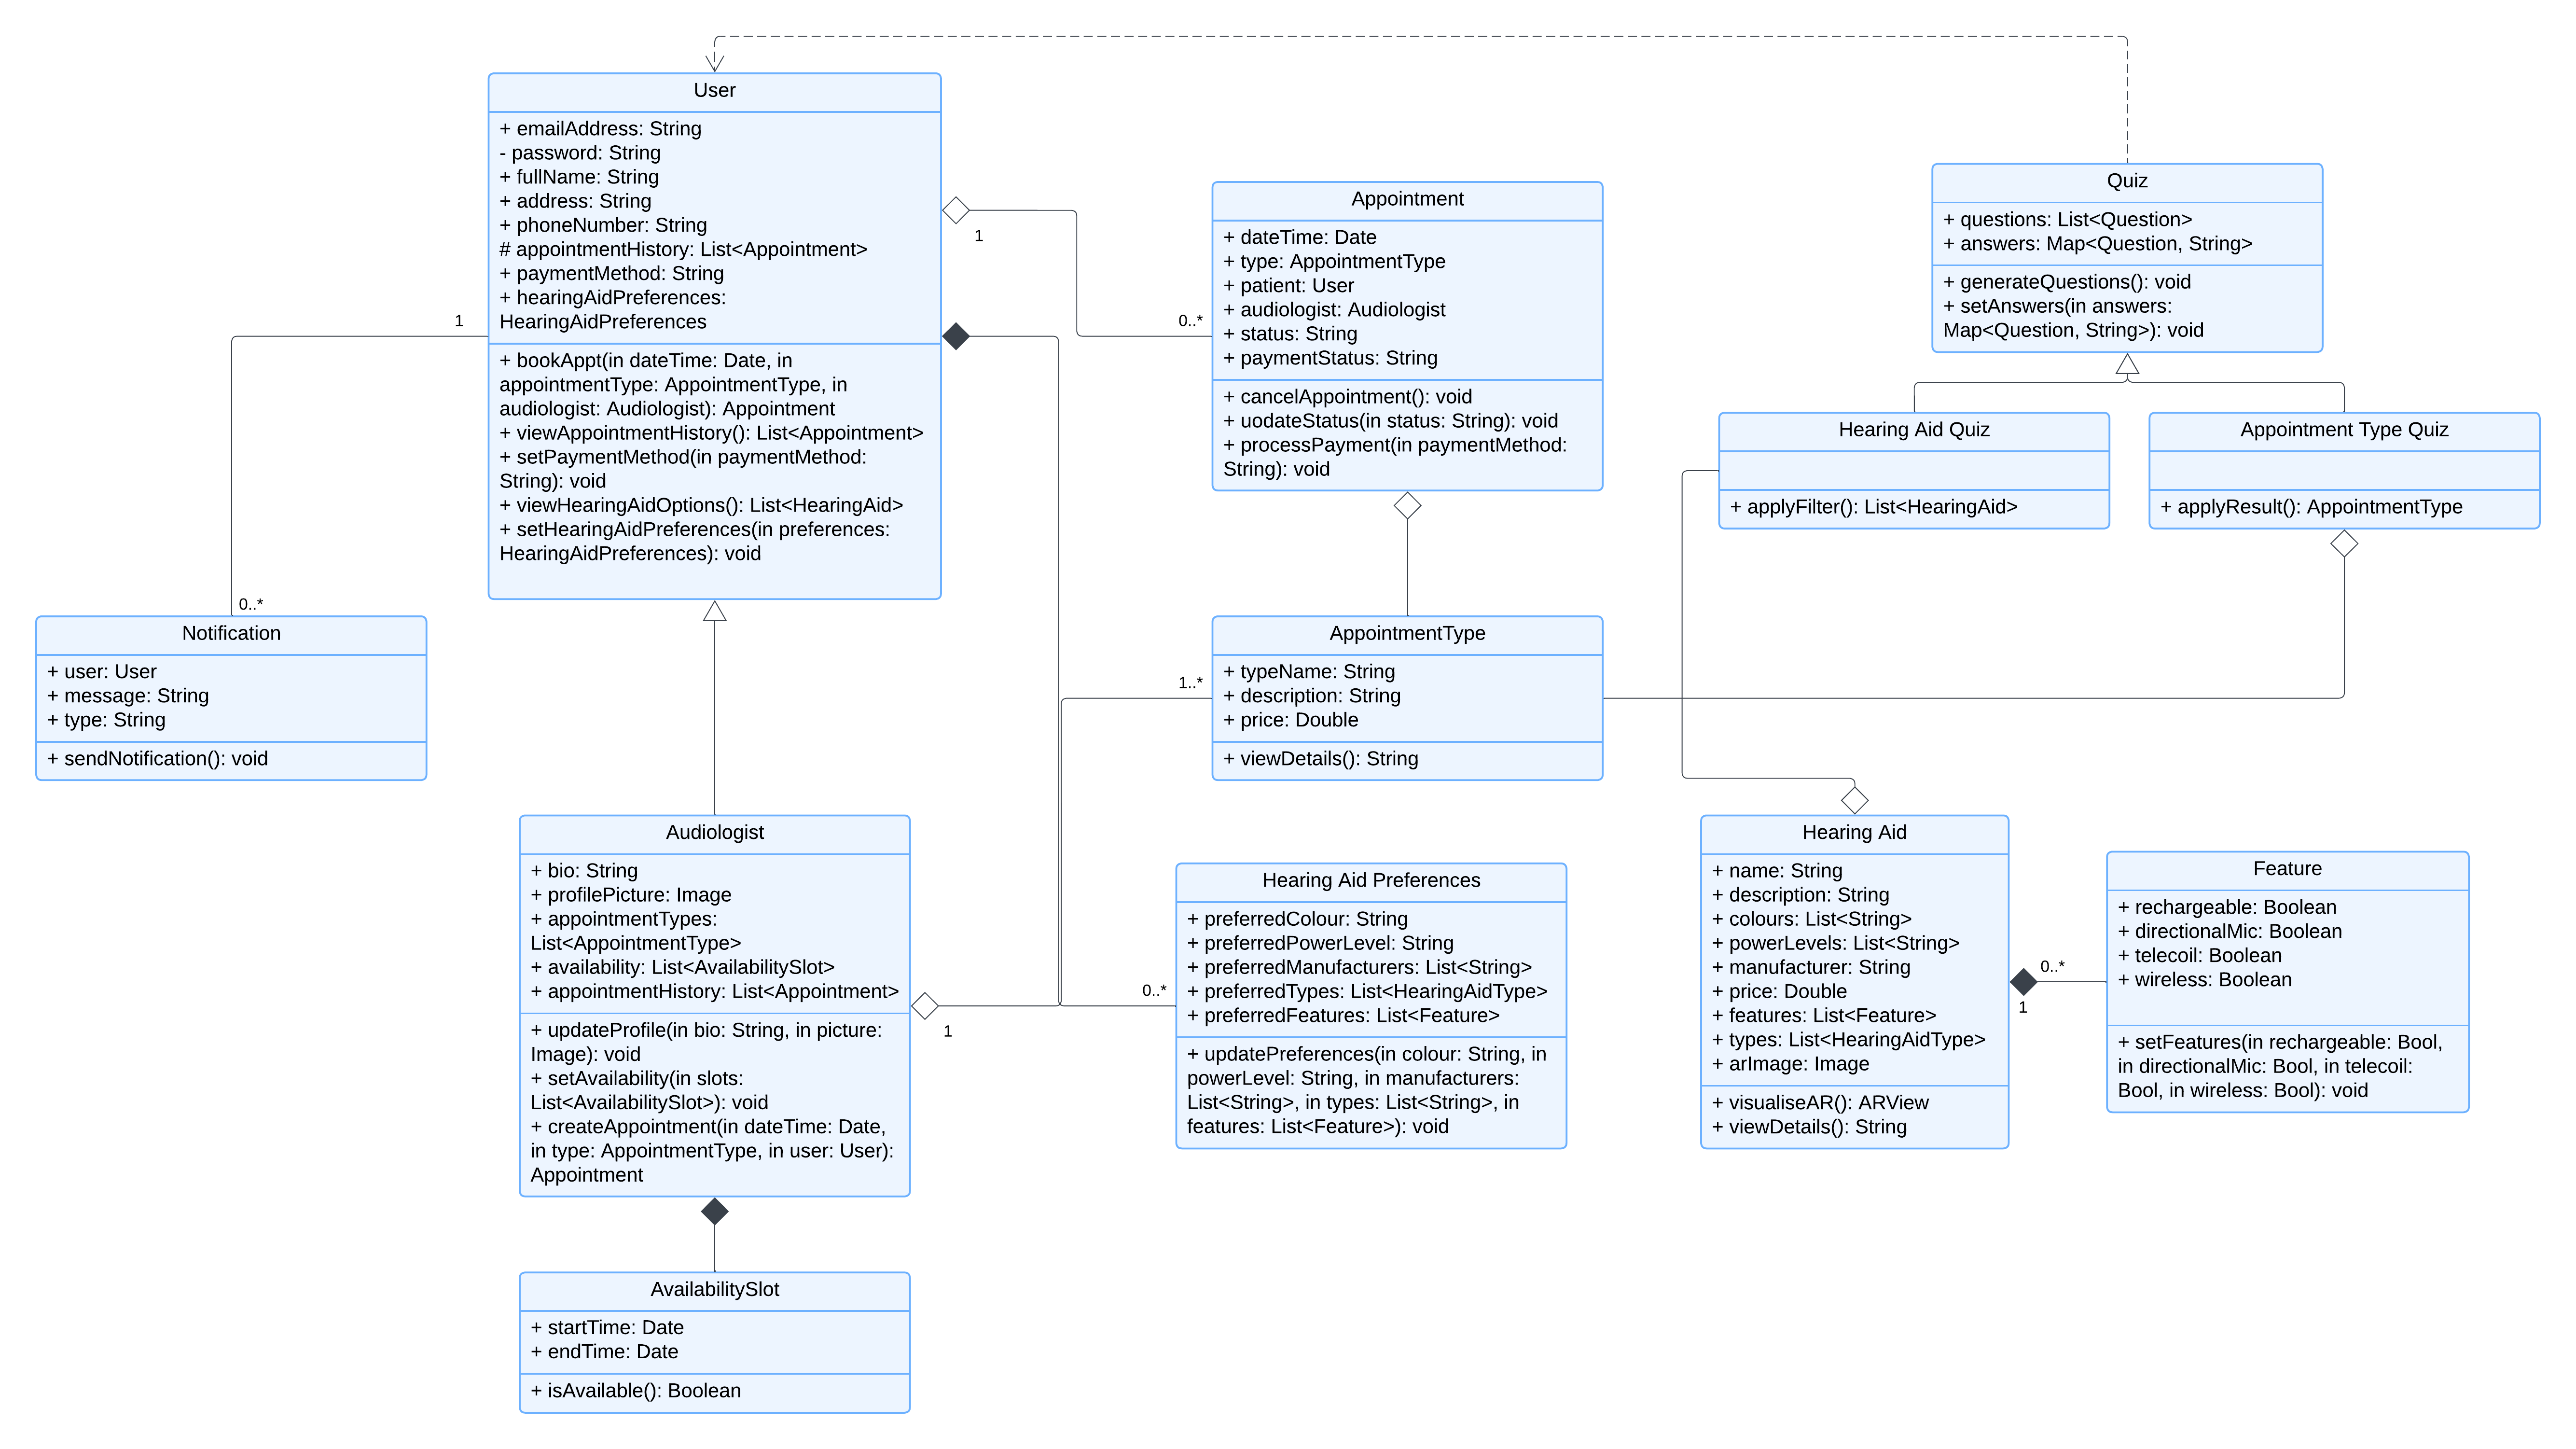
\includegraphics[width=\textwidth]{classdiagram.png}
    \caption{Class Diagram}
    \label{fig:class-diagram}
\end{figure}

The class diagram above represents the overall architecture of the hearing aid application. The User class contains essential attributes like email, password, and appointment history, which are inherited by the Audiologist subclass, adding specific details like bio, picture, and appointment availability. The Appointment class is linked to both the User and Audiologist, allowing users to book appointments and audiologists to manage their schedules. The Hearing Aid class includes attributes such as picture, price, and features, which are tied to user preferences through quizzes. Quiz and its subclasses, Hearing Aid Quiz and Appointment Type Quiz, help users make informed decisions by filtering hearing aids or appointment types based on their responses. Notification ensures that users are informed about appointment updates and hearing aid arrivals.



\subsection{Entity-Relationship Diagram}
The Entity Relationship (ER) Model is a framework used to identify the key entities that need to be included in a database and how these entities are connected. It provides a visual representation of the database's overall structure, showing how different pieces of data relate to one another within the system. The ER model defines the logical organization of the database schema \cite{geeksforgeeks_er_model}.
\begin{figure}[H]
    \centering
    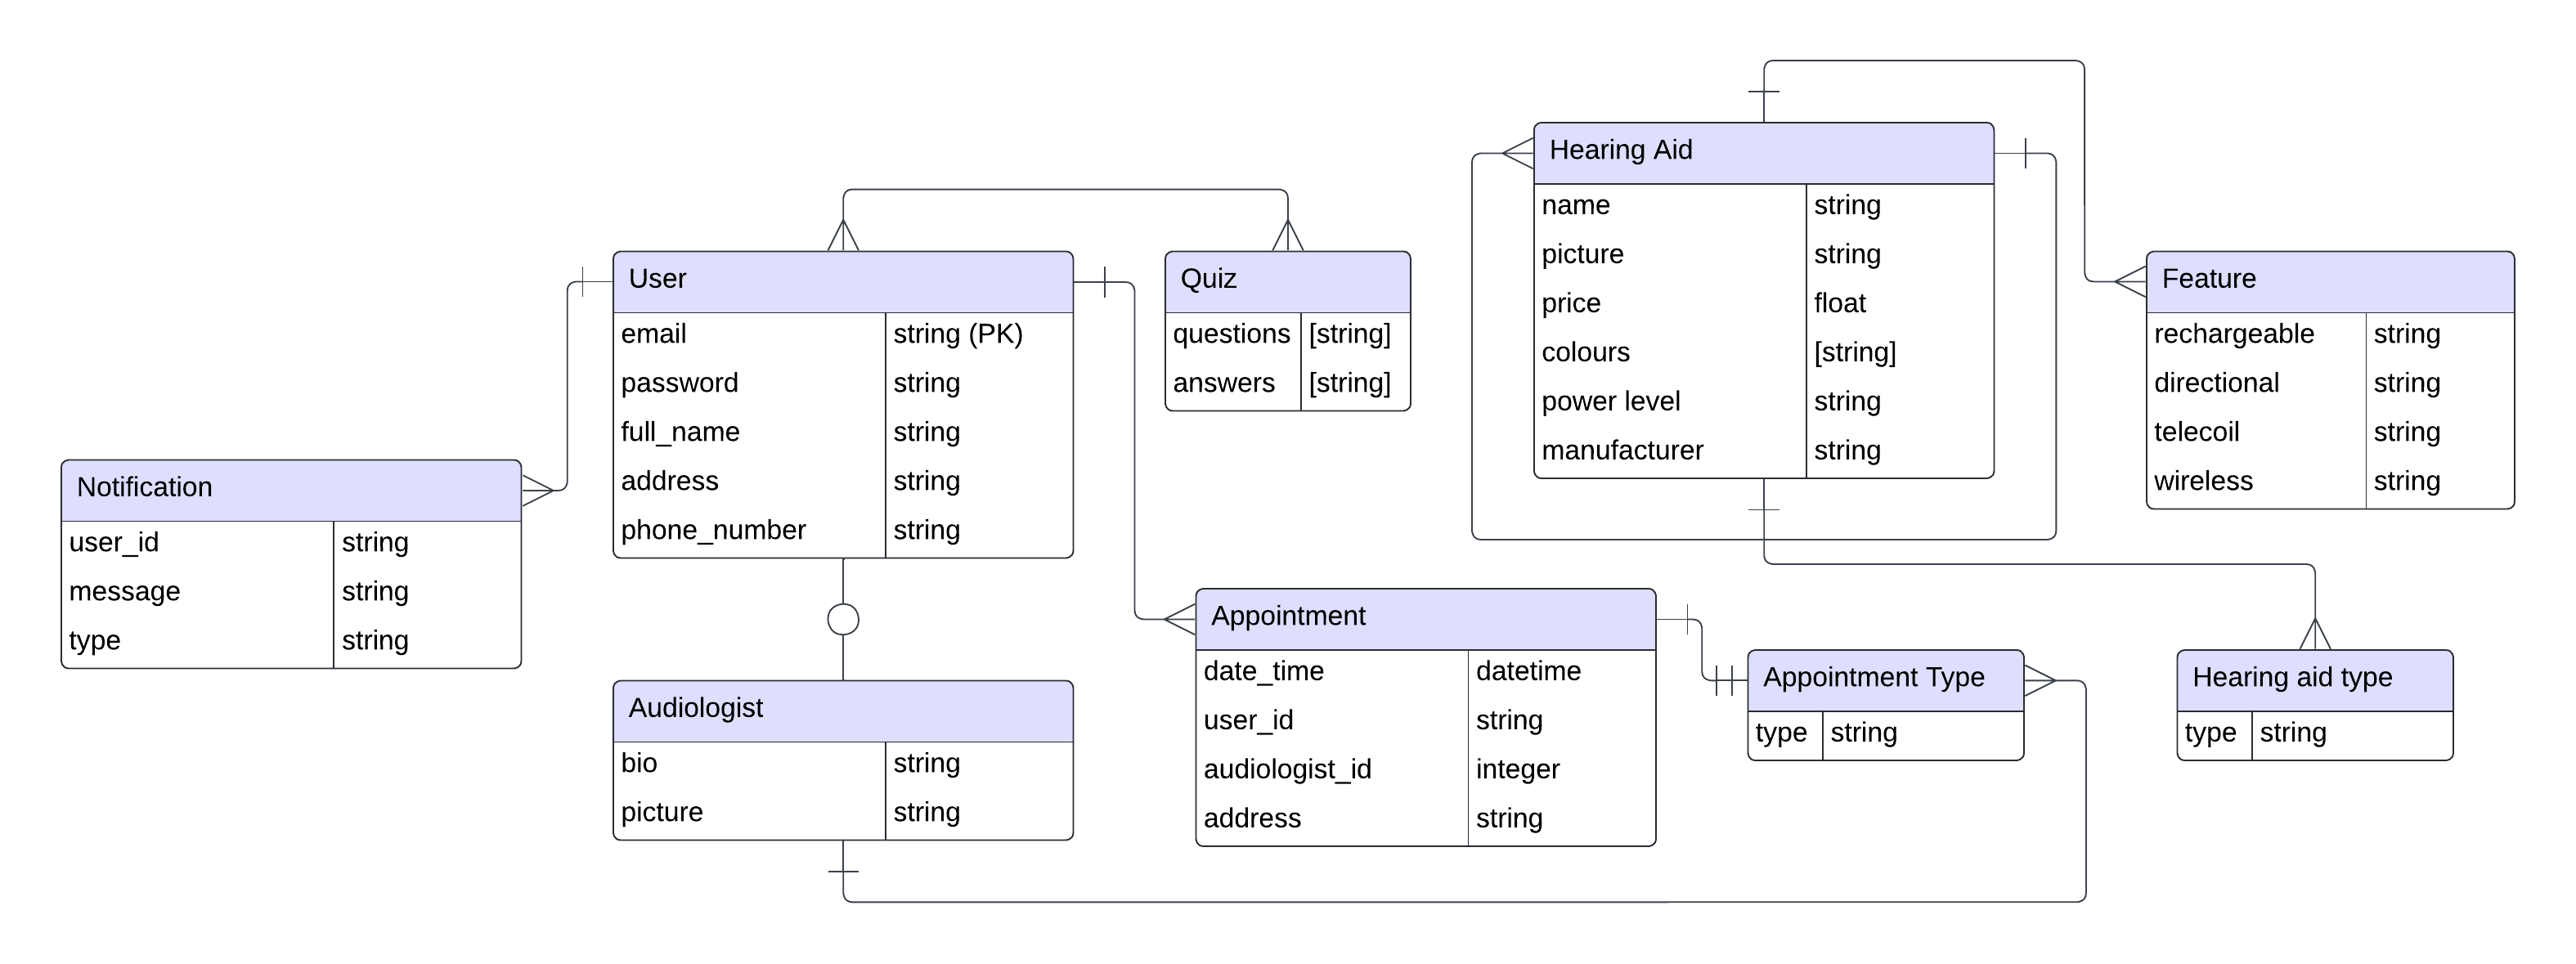
\includegraphics[width=\textwidth]{erd.png}
    \caption{Entity Relationship Diagram}
    \label{fig:erd-diagram}
\end{figure}

In the entity relationship diagram, there are several entities, including User, Audiologist, Appointment, Hearing Aid, Quiz, and Notification, along with the relationships between them. A User can have zero to many Appointments, and each Appointment is linked to exactly one User and one Audiologist. Audiologists can manage zero to many Appointments and can offer multiple types of appointments, but each Appointment is assigned to only one Audiologist. Users can also have zero to many Notifications, while each Notification is associated with one User. Users can answer quizzes like Hearing Aid Quiz and Appointment Type Quiz, and each quiz may have zero to many users. Hearing Aids are linked to many Users as preferences, forming a many-to-many relationship. Additionally, Audiologists can set their availability for different Appointments and manage their profiles, which include a bio and picture. Finally, the User can select from different Hearing Aids, which have various features, prices, and types, and users may prefer multiple hearing aids based on their needs.

\subsection{User Interface}
This subsection includes the draft wireframes before the application development for both Desktop and Mobile.

\subsubsection{Desktop User Interface}
\begin{figure}[H]
    \centering
    
\includegraphics[width=\textwidth]{desktop.png}
    \caption{Desktop User Interface}
    \label{fig:desktop}
\end{figure}

\subsubsection{Mobile User Interface}
\begin{figure}[H]
    \centering
    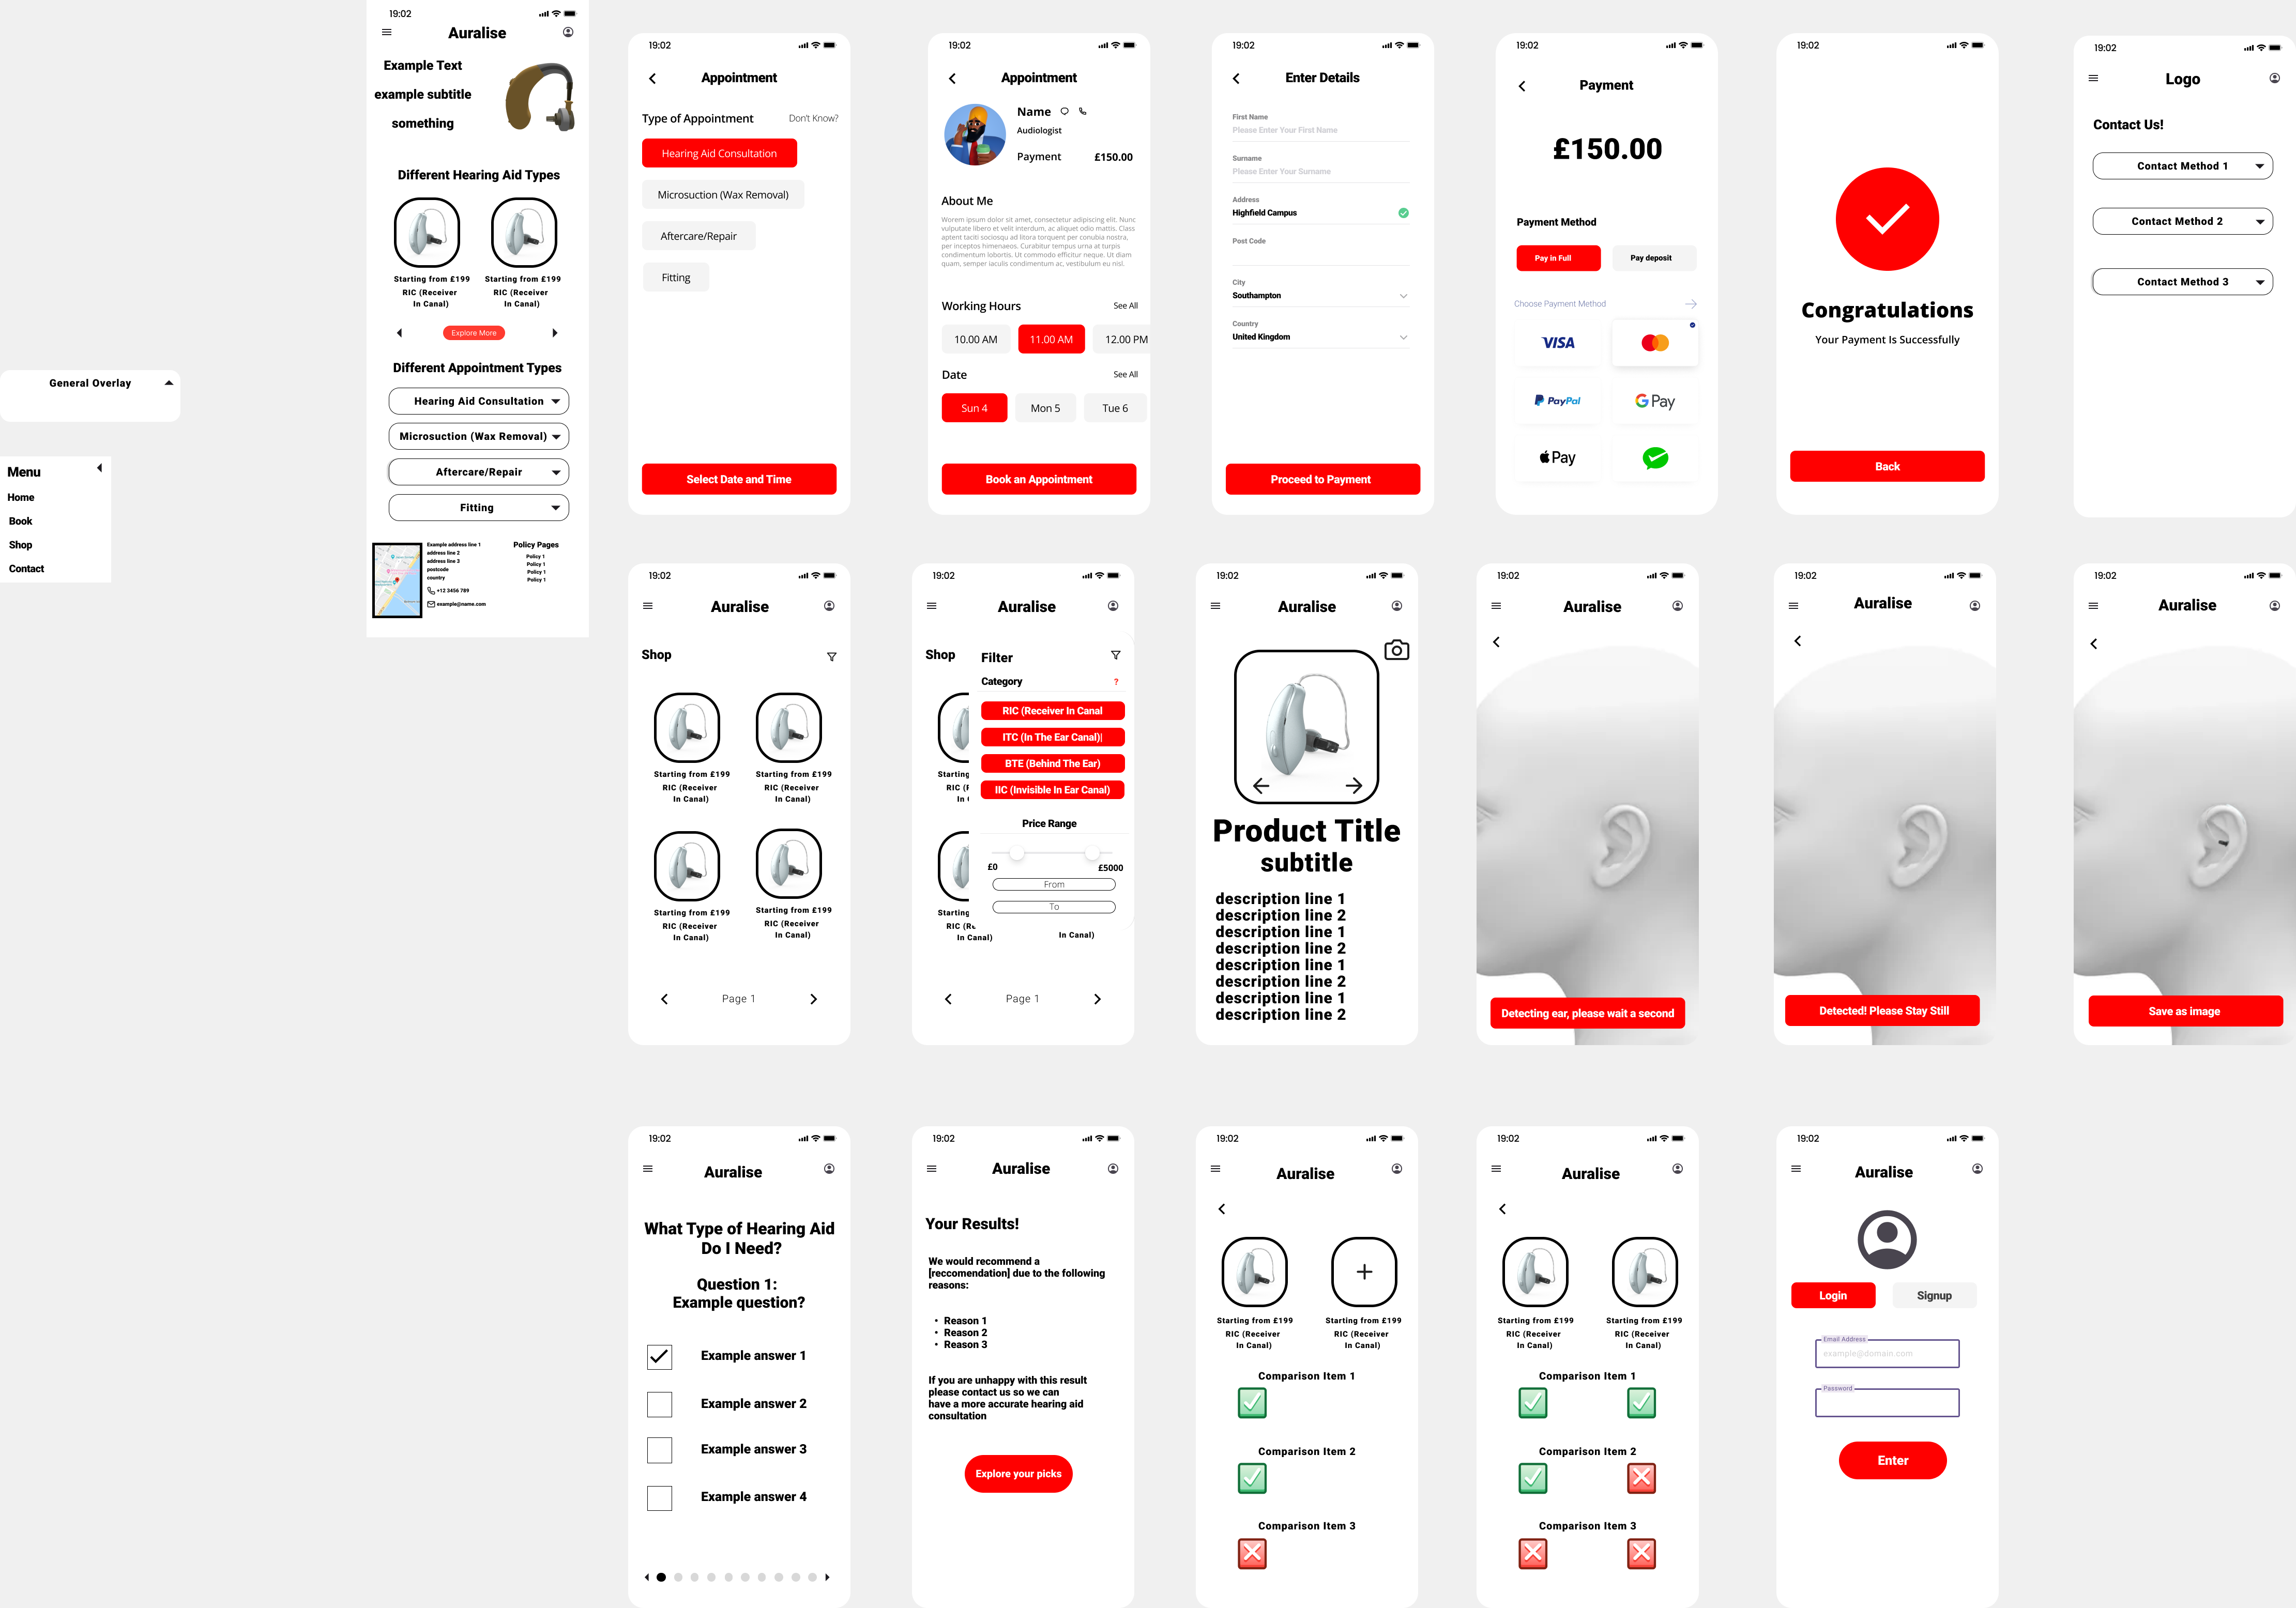
\includegraphics[width=\textwidth]{mobile.png}
    \caption{Mobile User Interface}
    \label{fig:mobile}
\end{figure}

Figures ~\ref{fig:desktop} and ~\ref{fig:mobile} represent the user interfaces for the hearing aid application, designed for both desktop and mobile platforms. The Landing Page provides users with access to key features such as booking appointments, shopping for hearing aids, and taking quizzes. The Book Page allows users to schedule appointments with audiologists, while the Confirmation of Booking Page displays appointment details. On both platforms, the Payment Page facilitates appointment payments, and the Contact Page enables users to reach the business for support. The Shop Page allows browsing of available hearing aids, and the Product Page offers detailed information about each hearing aid. Users can compare different hearing aids using the Comparison Page. The Try On Hearing Aid Page features augmented reality on mobile, enabling users to virtually try on hearing aids, while desktop users can upload an image to see how the hearing aids will look. The Type of Hearing Aid Quiz Page helps users select the right hearing aid, and the Type of Appointments Quiz Page guides them to the appropriate appointment type. The Quiz Results General Page displays quiz results to assist in decision-making. The Login/Signup Page provides user account access, and General Overlays enable collapsing sections for a cleaner interface. The mobile interface is optimized for touch interactions, with some features like AR enhanced for mobile use, while the desktop version is designed for a more traditional browsing experience.

\newpage

\fancyhead[L]{} 
\fancyhead[L]{\textbf{6 Implementation} \vspace{1pt}} % "CONTENTS" title

\section{Implementation}
This section details the implementation of the Hearing-centric application, providing a comprehensive overview of each development phase—both front-end and back-end—that contributed to the final product.

\subsection{Kotlin Backend Directory Structure}

\begin{figure}[H]
    \centering
    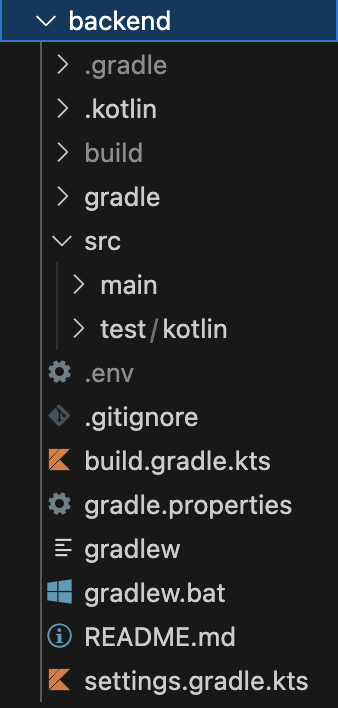
\includegraphics[width=0.3\textwidth]{backend_directory_structure.png}
    \caption{Directory structure of the Kotlin backend for the Hearing Aid Platform}
    \label{fig:backend-structure}
\end{figure}

\noindent
Figure~\ref{fig:backend-structure} illustrates the directory structure of the Kotlin backend used in this project.

The backend follows a standard project layout tailored for a Ktor-based application \cite{ktor_project_2024}. The root directory includes essential configuration files such as \texttt{build.gradle.kts}, which specifies dependencies and build settings, and \texttt{.env}, which stores environment variables for database connections and other configurations.

Inside the \texttt{src} directory, there are two primary subdirectories: \texttt{main} and \texttt{test}. The \texttt{main} directory contains the core application code, while \texttt{test} holds unit and integration tests. Within \texttt{main}, the \texttt{kotlin} folder includes the Kotlin source code, organized into several key packages:

\begin{itemize}
    \item \texttt{controller}: Handles incoming HTTP requests and defines API endpoints.
    \item \texttt{service} and \texttt{services}: Contain business logic and core service classes.
    \item \texttt{model} and \texttt{models}: Define data models and application entities.
    \item \texttt{repository}: Implements data access logic for interacting with Azure Cosmos DB.
    \item \texttt{routes}: Configures API routes for the Ktor framework.
    \item \texttt{config}: Contains configuration classes for initializing application components.
    \item \texttt{utils}: Provides utility functions and helper classes.
\end{itemize}

The \texttt{resources} directory stores configuration files and static assets. The \texttt{Application.kt} file serves as the application's entry point, and \texttt{Routing.kt} defines the main routing logic.

The Gradle build system, managed via the root directory, handles dependency management, project building, and deployment \cite{gradle_guide_2024}. This organized structure adheres to Kotlin best practices, ensuring maintainability and scalability.


\subsection{Development Environment}

This section outlines the tools, libraries, and configurations used during the development of the Hearing Aid Platform.

\subsubsection{Environment Setup}

The development of the Hearing Aid Platform utilized a range of tools and services across both frontend and backend environments:

\begin{itemize}
    
    \item Visual Studio Code: Used for frontend development with React and TypeScript, supported by extensions for TypeScript, React, and ESLint to enable intelligent code completion, linting, and debugging. 
    
    \item Azure Portal: Manages Azure Cosmos DB resources, configures access policies, and monitors database performance for backend data storage.
    
    \item GitHub: Facilitates version control, collaborative development, and CI/CD integration for automated testing and deployment.
    
    \item Postman: Assists in testing and documenting REST APIs, ensuring endpoints function correctly prior to frontend integration.
\end{itemize}

\subsubsection{Backend Libraries}

The backend, developed using Kotlin and Ktor, leverages a range of libraries as defined in the \texttt{build.gradle.kts} file:

\begin{lstlisting}[language=, caption={Backend \texttt{build.gradle.kts} Dependencies}, label={lst:gradle-deps}]
dependencies {
    implementation("io.ktor:ktor-server-core-jvm")
    implementation("io.ktor:ktor-server-netty")
    implementation("ch.qos.logback:logback-classic:$logback_version")
    implementation("io.ktor:ktor-server-core")
    implementation("io.ktor:ktor-server-content-negotiation:$kotlin_version")
    implementation("io.ktor:ktor-server-config-yaml")
    implementation("com.azure:azure-cosmos:4.9.0")
    implementation("io.github.cdimascio:dotenv-kotlin:6.2.2")
    implementation("io.ktor:ktor-serialization-kotlinx-json:2.2.4")
    implementation("io.ktor:ktor-serialization-kotlinx-json:$kotlin_version")
    implementation("org.mindrot:jbcrypt:0.4")
    
    // Email dependencies
    implementation("com.sun.mail:javax.mail:1.6.2")
    implementation("javax.activation:activation:1.1.1")
    
    // Image processing
    implementation("org.imgscalr:imgscalr-lib:4.2")
    
    testImplementation("io.ktor:ktor-server-test-host")
    testImplementation("org.jetbrains.kotlin:kotlin-test-junit:$kotlin_version")
    implementation("io.ktor:ktor-server-cors:$kotlin_version")
}
\end{lstlisting}

\begin{itemize}
    \item \texttt{ktor-server-core}, \texttt{ktor-server-netty}, etc.: Provide core server functionality, HTTP routing, and Netty engine support.
    \item \texttt{azure-cosmos}: Enables integration with Azure Cosmos DB for persistent storage.
    \item \texttt{dotenv-kotlin}: Handles environment variables securely.
    \item \texttt{jbcrypt}: Implements password hashing for secure authentication.
    \item \texttt{javax.mail}, \texttt{activation}: Enable email features for appointment notifications.
    \item \texttt{imgscalr-lib}: Supports image manipulation used in the AR component.
\end{itemize}

\subsubsection{Frontend Libraries}

The frontend is built using React with TypeScript and a suite of modern libraries defined in the \texttt{package.json} file:

\begin{lstlisting}[language=, caption={Frontend \texttt{package.json} Dependencies}, label={lst:frontend-deps}]
"dependencies": {
  "@dnd-kit/core": "^6.3.1",
  "@fortawesome/react-fontawesome": "^0.2.2",
  "@react-three/drei": "^9.121.4",
  "@react-three/fiber": "^8.17.14",
  "axios": "^1.8.1",
  "bootstrap": "^5.3.3",
  "clsx": "^2.1.1",
  "dotenv": "^16.4.7",
  "framer-motion": "^12.4.7",
  "leva": "^0.10.0",
  "lucide-react": "^0.474.0",
  "microsoft-cognitiveservices-speech-sdk": "^1.43.1",
  "react": "^18.3.1",
  "react-bootstrap": "^2.10.9",
  "react-burger-menu": "^3.1.0",
  "react-dom": "^18.3.1",
  "react-icons": "^5.4.0",
  "react-router-dom": "^7.1.3",
  "rsuite": "^5.77.0",
  "tailwind-merge": "^2.6.0",
  "three": "^0.172.0",
  "vite-plugin-pwa": "^0.21.1",
  "workbox-window": "^7.3.0"
}
\end{lstlisting}

\begin{itemize}
    \item \texttt{react-three/fiber}, \texttt{three}: Power 3D rendering for AR visualization and product previews.
    \item \texttt{microsoft-cognitiveservices-speech-sdk}: Supports speech-based interaction features.
    \item \texttt{axios}: Handles RESTful communication with the backend.
    \item \texttt{framer-motion}: Adds modern UI animations and transitions.
    \item \texttt{bootstrap}, \texttt{rsuite}: Provide responsive UI components.
    \item \texttt{vite-plugin-pwa}, \texttt{workbox-window}: Enable PWA capabilities like offline caching.
\end{itemize}

Both environments are configured to streamline development and deployment, promoting maintainability and performance throughout the application's lifecycle.

\subsection{Application User Interface}
This section focuses on the user interface of the Hearing Aid Platform. The UI has been designed to be responsive, accessible, and intuitive for users of all technical abilities. The application uses React Bootstrap and custom CSS components that adapt to different screen sizes, ensuring a consistent experience across desktop, tablet, and mobile devices. Special emphasis has been placed on accessibility features to accommodate users with hearing impairments.

The following figures illustrate the key screens that users of the Hearing Aid Platform can access. The application interface follows modern design principles with a focus on simplicity and clarity to help users navigate the hearing healthcare journey seamlessly.

Note: The Application User Interface has been refined through multiple iterations of user testing with both audiologists and potential hearing aid users to ensure optimal usability.

\subsubsection{Home Page and Navigation}

\begin{figure}[H]
\centering
\begin{minipage}{0.45\textwidth}
    \centering
    
\includegraphics[height=0.4\textheight]{mobile_home.png}
    \caption{Mobile Home Page}
    \label{fig:mobile_home}
\end{minipage}
\hfill
\begin{minipage}{0.45\textwidth}
    \centering
    
\includegraphics[height=0.5\textheight]{desktop_home.png}
    \caption{Desktop Home Page}
    \label{fig:desktop_home}
\end{minipage}
\end{figure}

\begin{figure}[H]
    \centering
    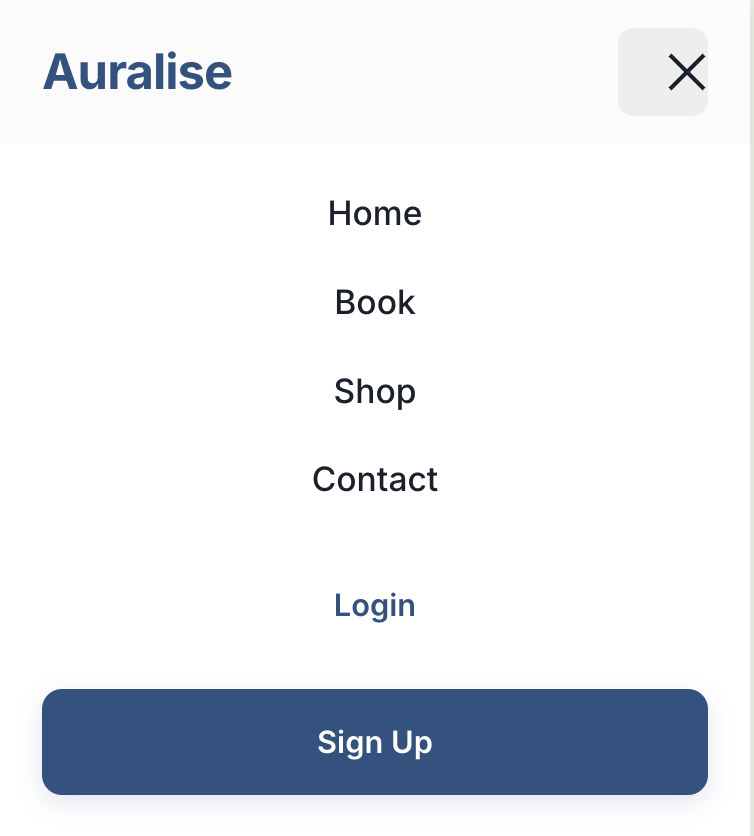
\includegraphics[height=0.2\textheight]{mobile_navigation.png}
    \caption{Mobile Navigation}
    \label{fig:mobile_navigation}
\end{figure}

\begin{figure}[H]
\centering
\begin{minipage}{0.45\textwidth}
    \centering
    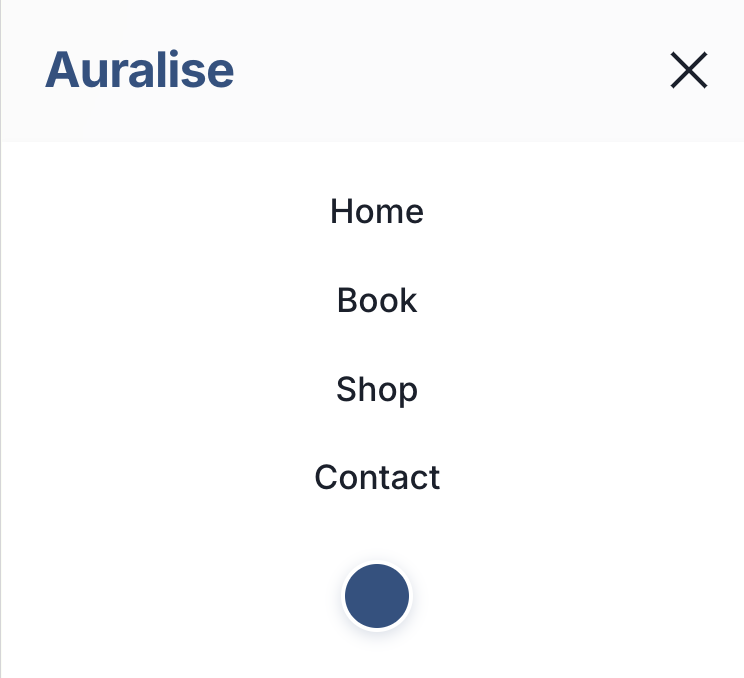
\includegraphics[height=0.2\textheight]{login_status_mobile.png}
    \caption{Login Status Mobile}
    \label{fig:login_status_mobile}
\end{minipage}
\hfill
\begin{minipage}{0.45\textwidth}
    \centering
    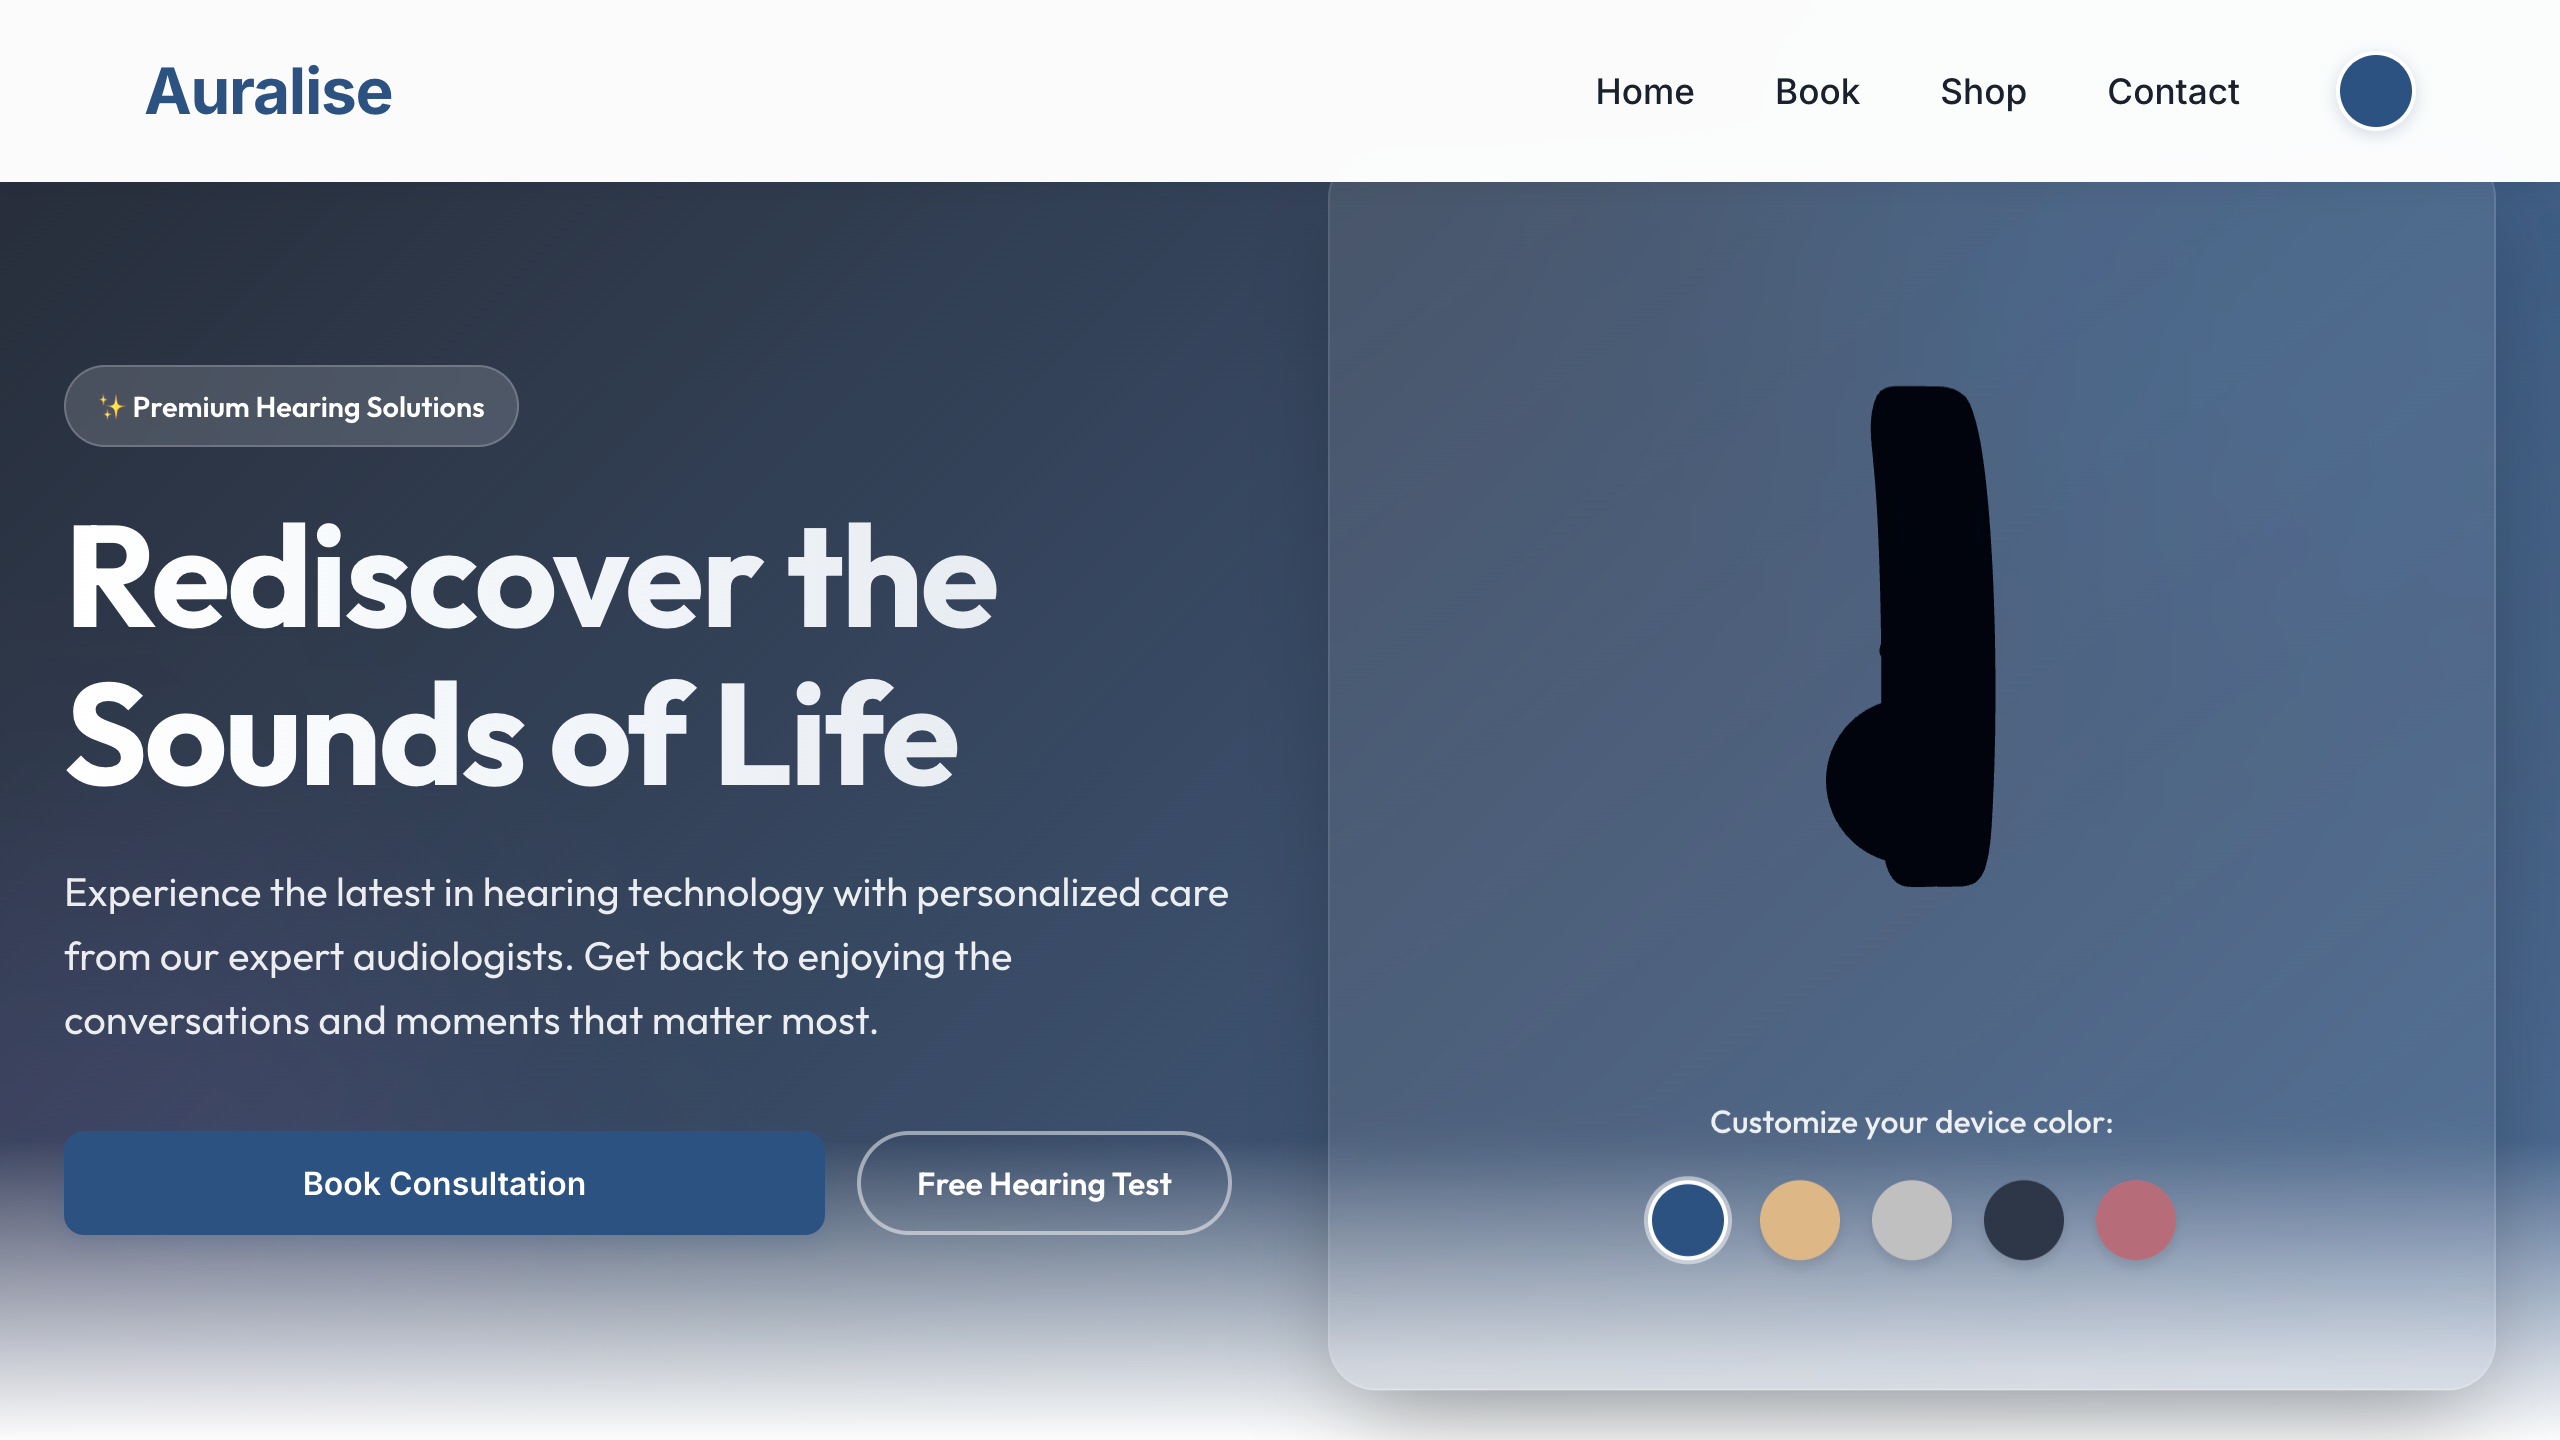
\includegraphics[height=0.15\textheight]{login_status_desktop.png}
    \caption{Login Status Desktop}
    \label{fig:login_status_desktop}
\end{minipage}
\end{figure}

As shown in Figures~\ref{fig:mobile_home} and~\ref{fig:desktop_home}, the Home page serves as the main entry point to the application, featuring a hero section with a 3D interactive hearing aid model that users can customize with different colors. The 3D model utilizes Three.js to provide a realistic preview of hearing aid devices. Below the hero section, users can quickly access core features: hearing test, appointment booking, product browsing, and educational resources.

The navigation system includes a responsive menu that adapts to different screen sizes, collapsing into a hamburger menu on mobile devices, as shown in Figure~\ref{fig:mobile_navigation}. The user's login status is indicated in the top corner, with quick access to profile settings for logged-in users or login/signup options for new visitors as shown in Figures~\ref{fig:login_status_mobile} and~\ref{fig:login_status_desktop}.

\subsubsection{Login and Registration}

\begin{figure}[H]
\centering
\begin{subfigure}[b]{0.45\textwidth}
    \centering
    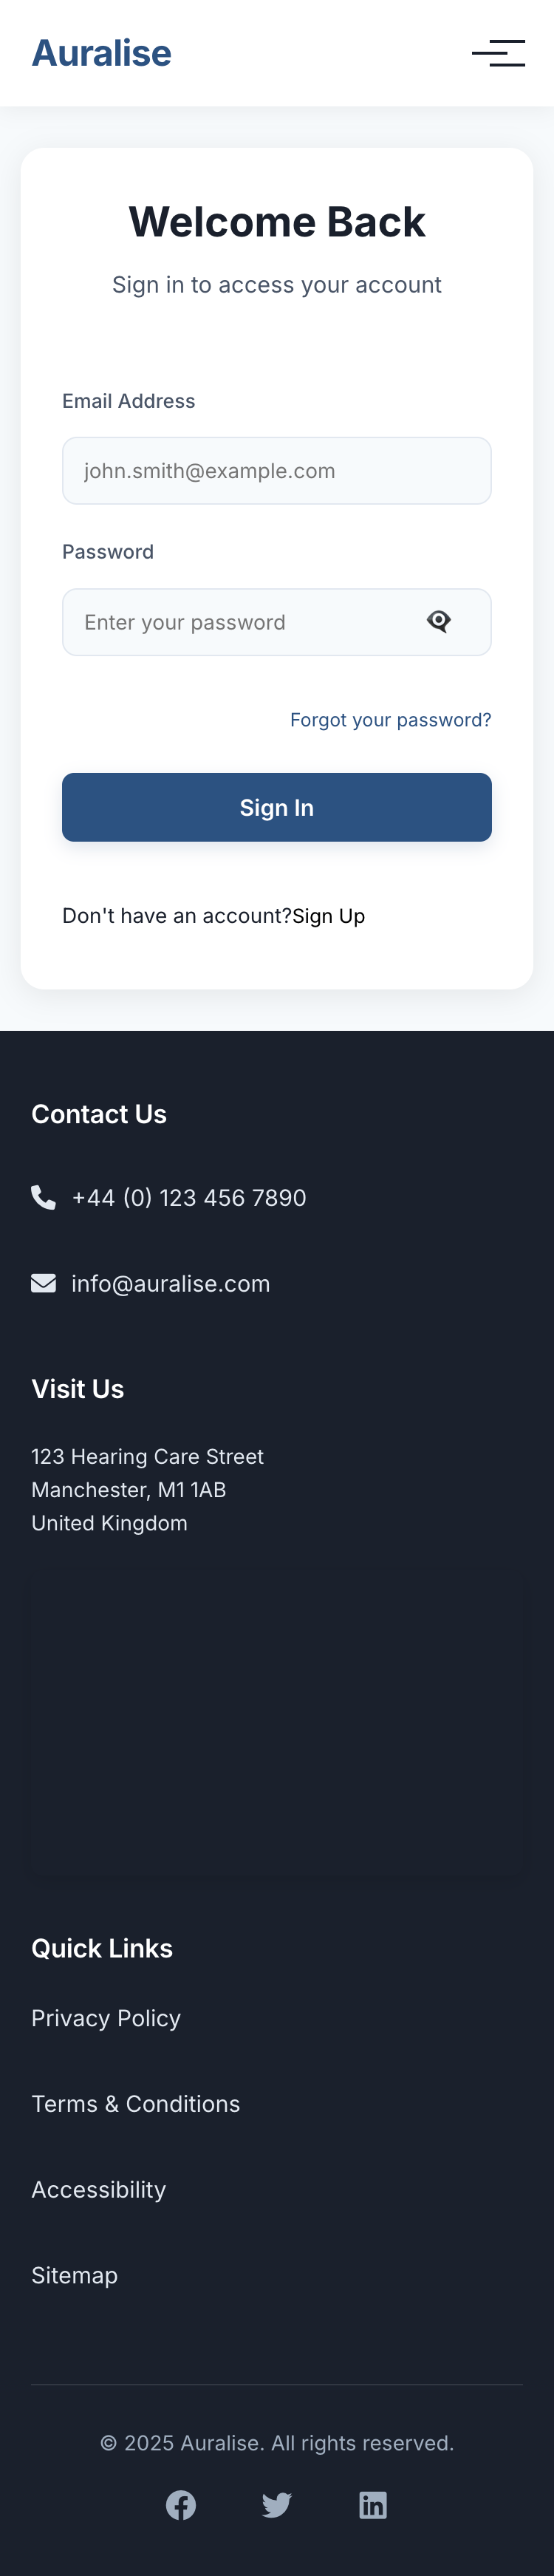
\includegraphics[width=\linewidth, height=0.6\textheight, keepaspectratio]{mobile_login.png}
    \caption{Mobile Login}
\end{subfigure}
\hfill
\begin{subfigure}[b]{0.45\textwidth}
    \centering
    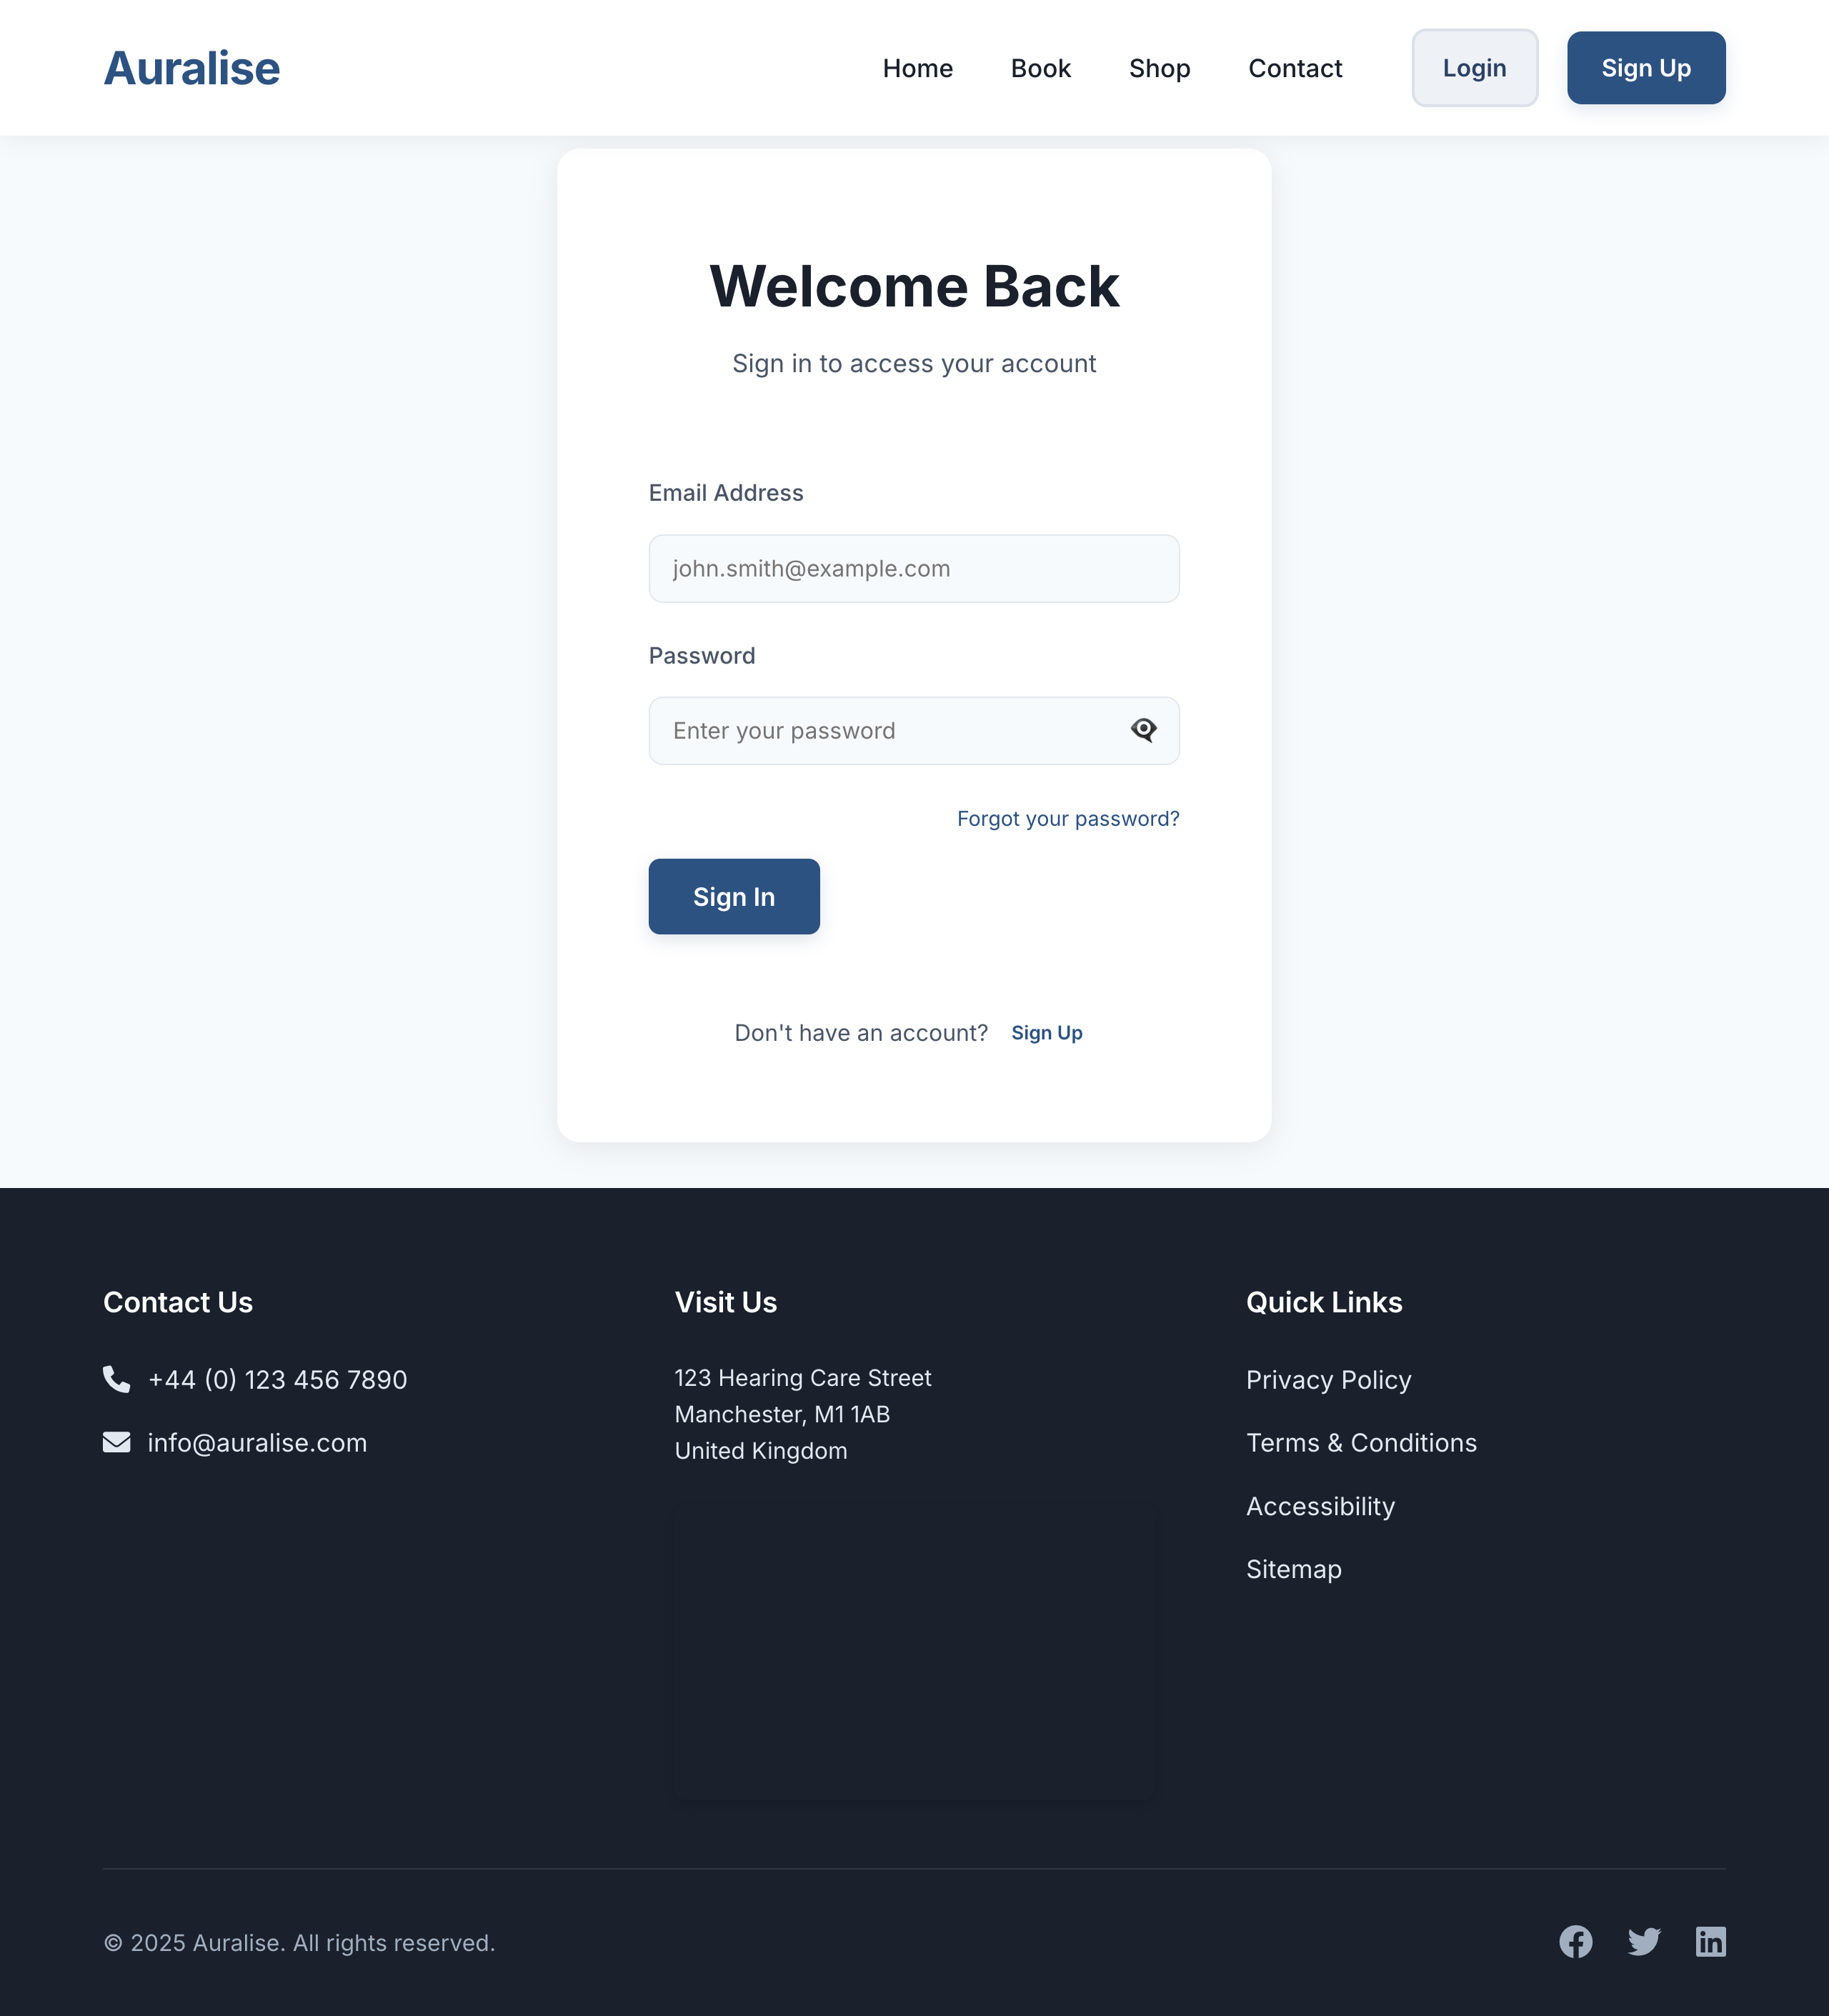
\includegraphics[width=\linewidth, height=0.6\textheight, keepaspectratio]{desktop_login.png}
    \caption{Desktop Login}
\end{subfigure}
\caption{Login Screen (Mobile and Desktop)}
\label{fig:login_page}
\end{figure}

\vspace{1em} % small vertical space between figures

\begin{figure}[H]
\centering
\begin{subfigure}[b]{0.45\textwidth}
    \centering
    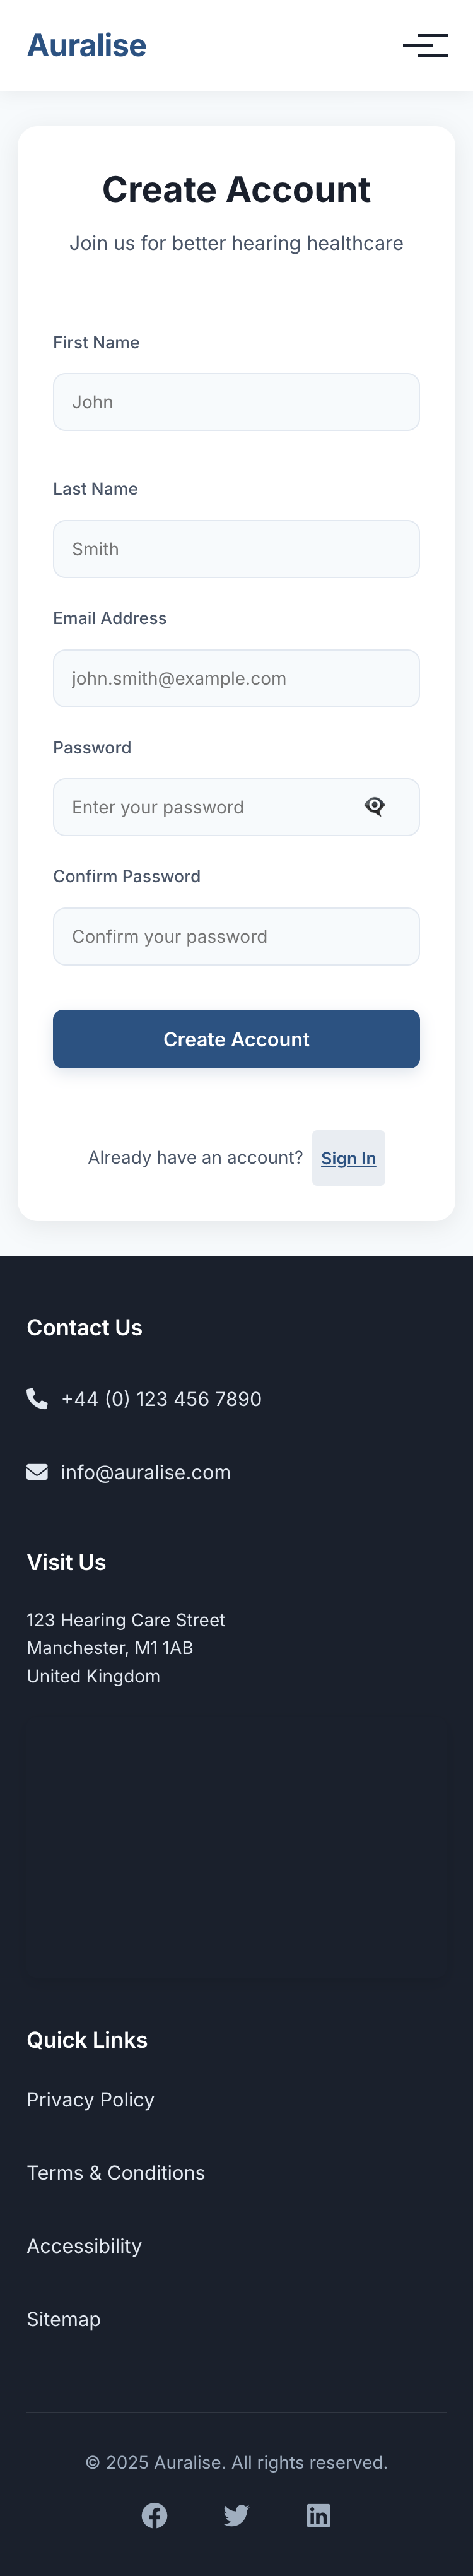
\includegraphics[width=\linewidth, height=0.6\textheight, keepaspectratio]{mobile_register.png}
    \caption{Mobile Registration}
\end{subfigure}
\hfill
\begin{subfigure}[b]{0.45\textwidth}
    \centering
    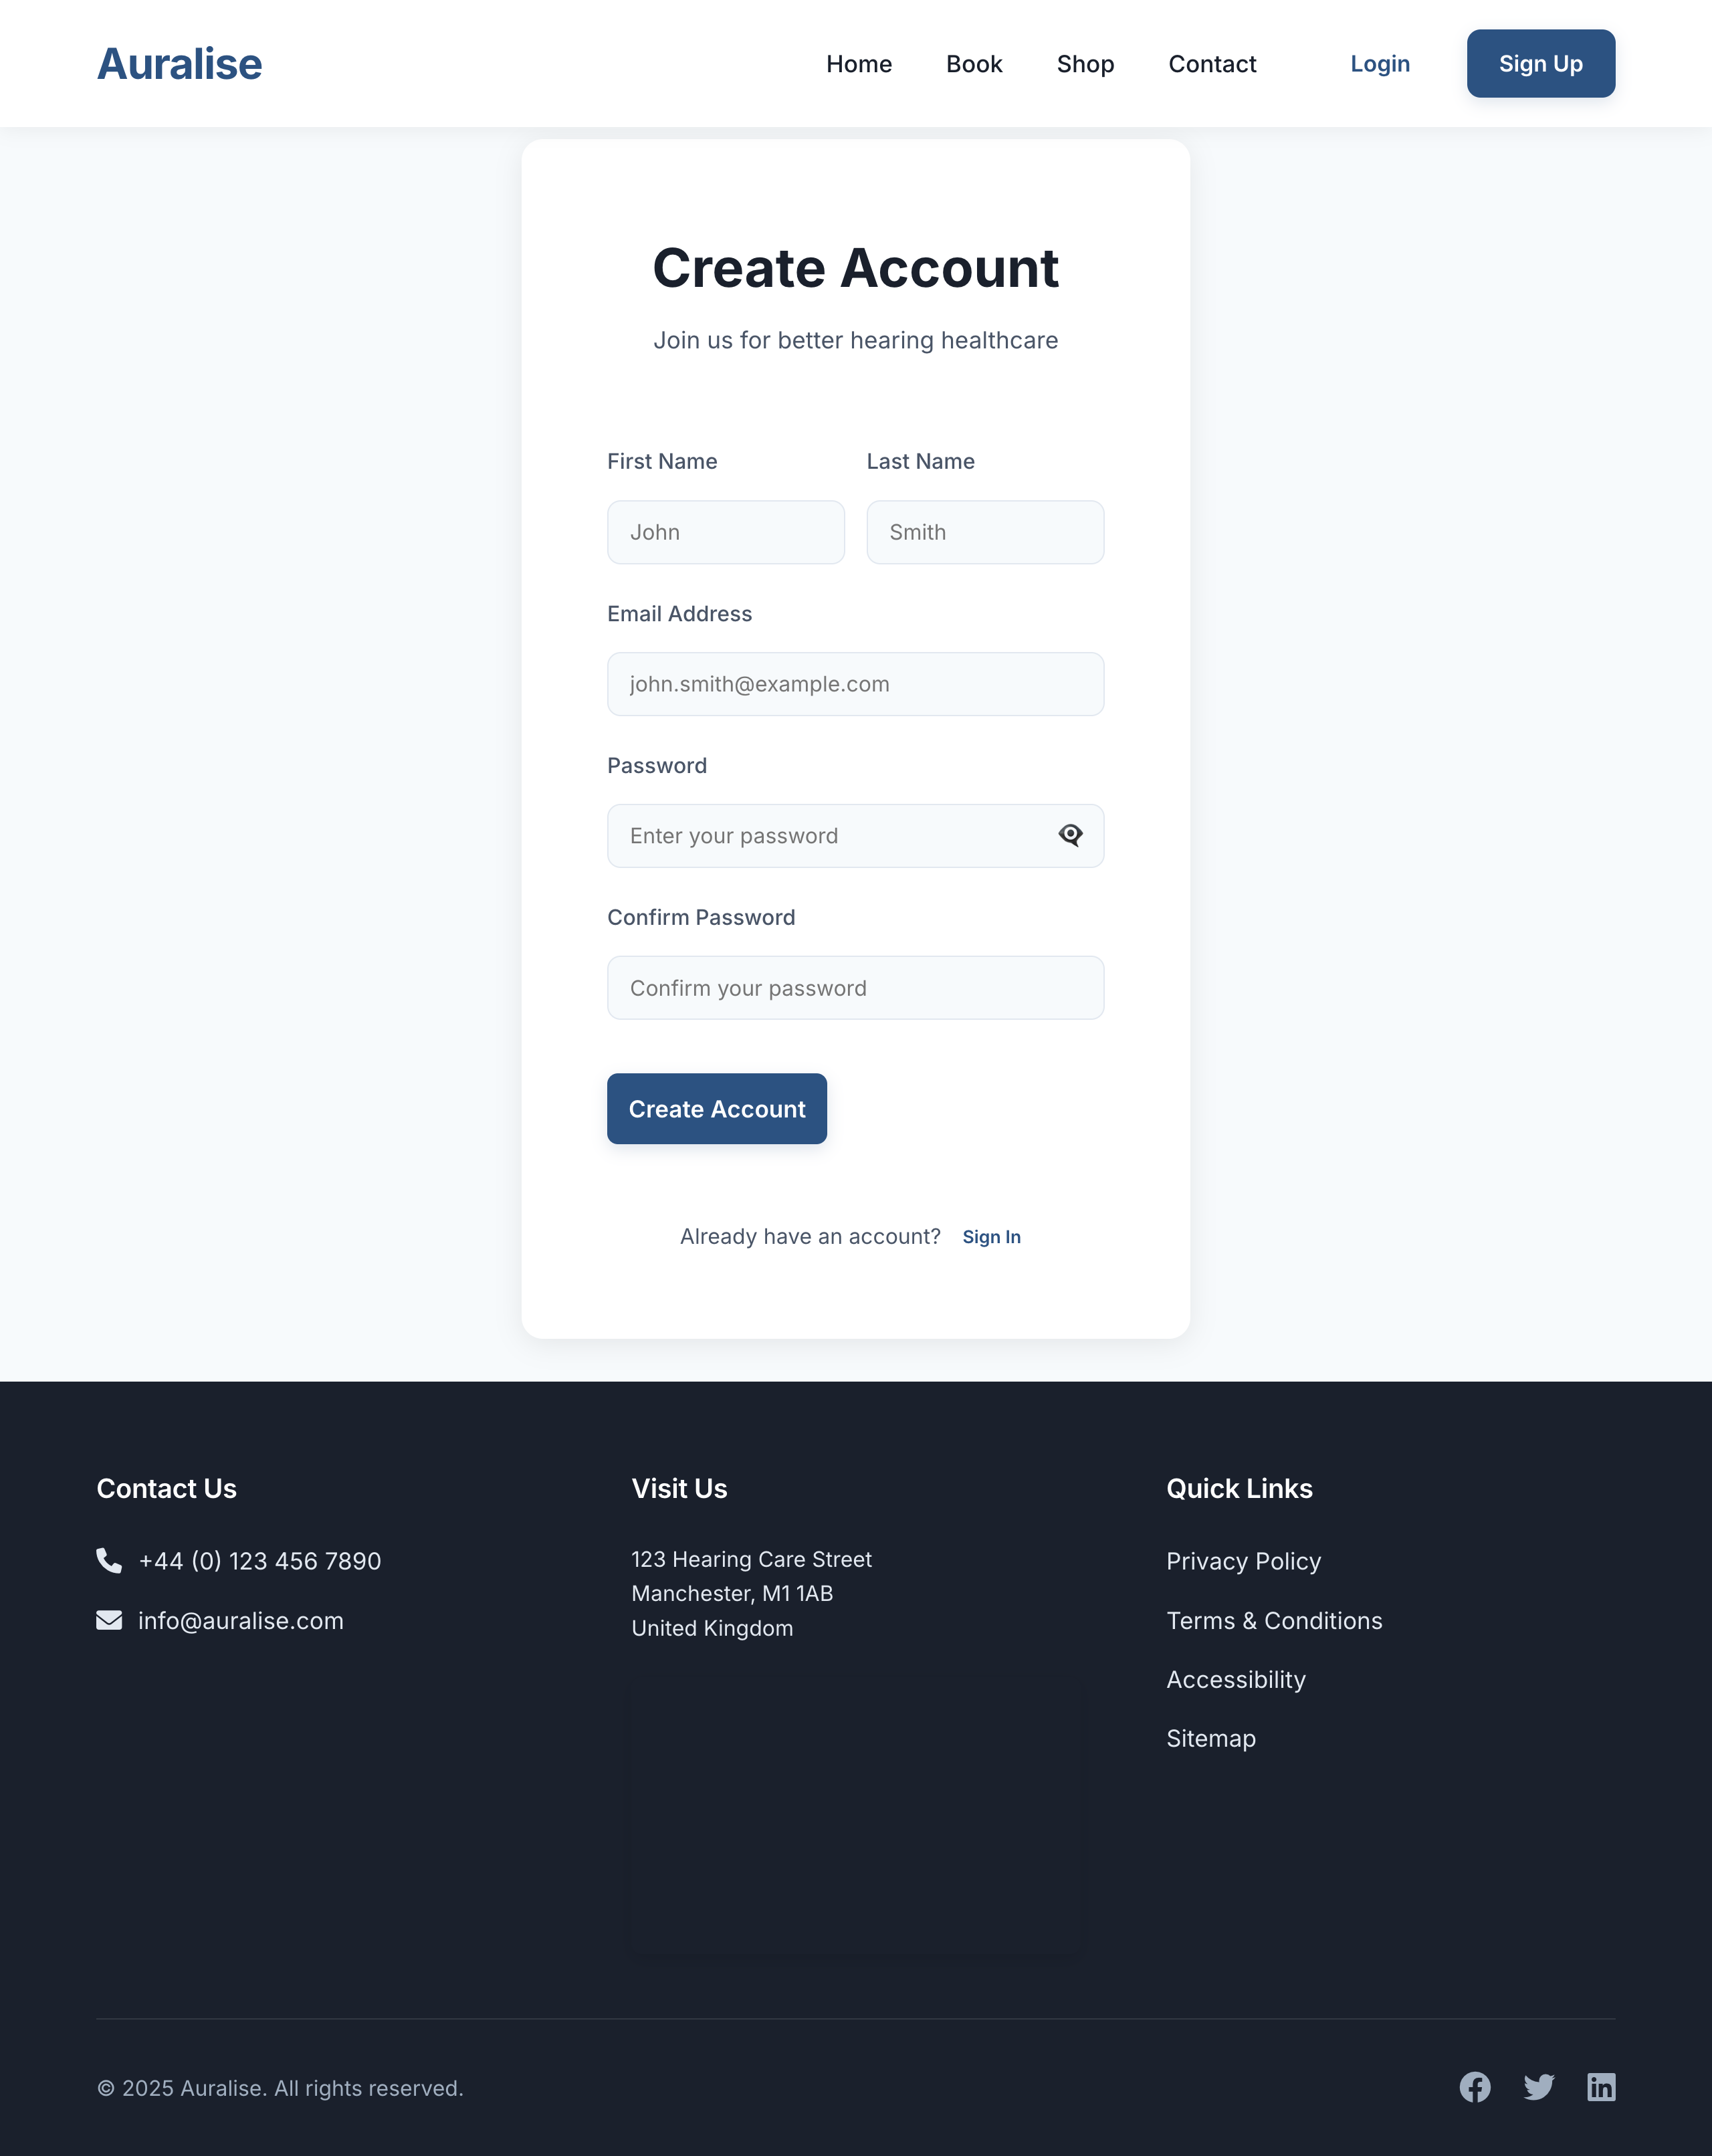
\includegraphics[width=\linewidth, height=0.6\textheight, keepaspectratio]{desktop_register.png}
    \caption{Desktop Registration}
\end{subfigure}
\caption{Registration Screen (Mobile and Desktop)}
\label{fig:register_page}
\end{figure}

\vspace{1em}

\begin{figure}[H]
\centering
\begin{subfigure}[b]{0.45\textwidth}
    \centering
    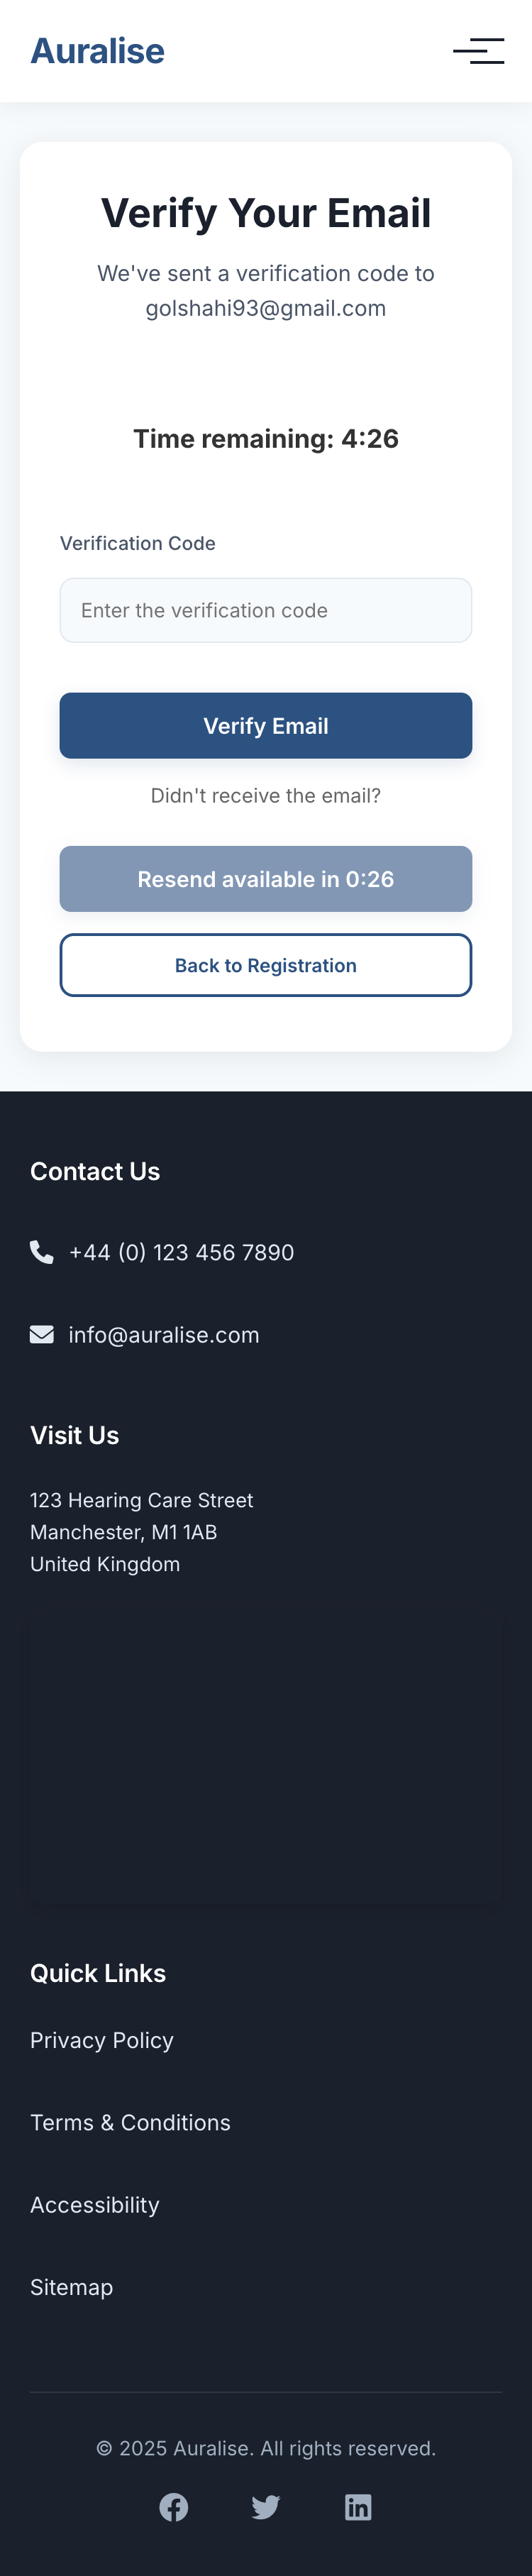
\includegraphics[width=\linewidth, height=0.6\textheight, keepaspectratio]{mobile_otp.png}
    \caption{Mobile OTP}
\end{subfigure}
\hfill
\begin{subfigure}[b]{0.45\textwidth}
    \centering
    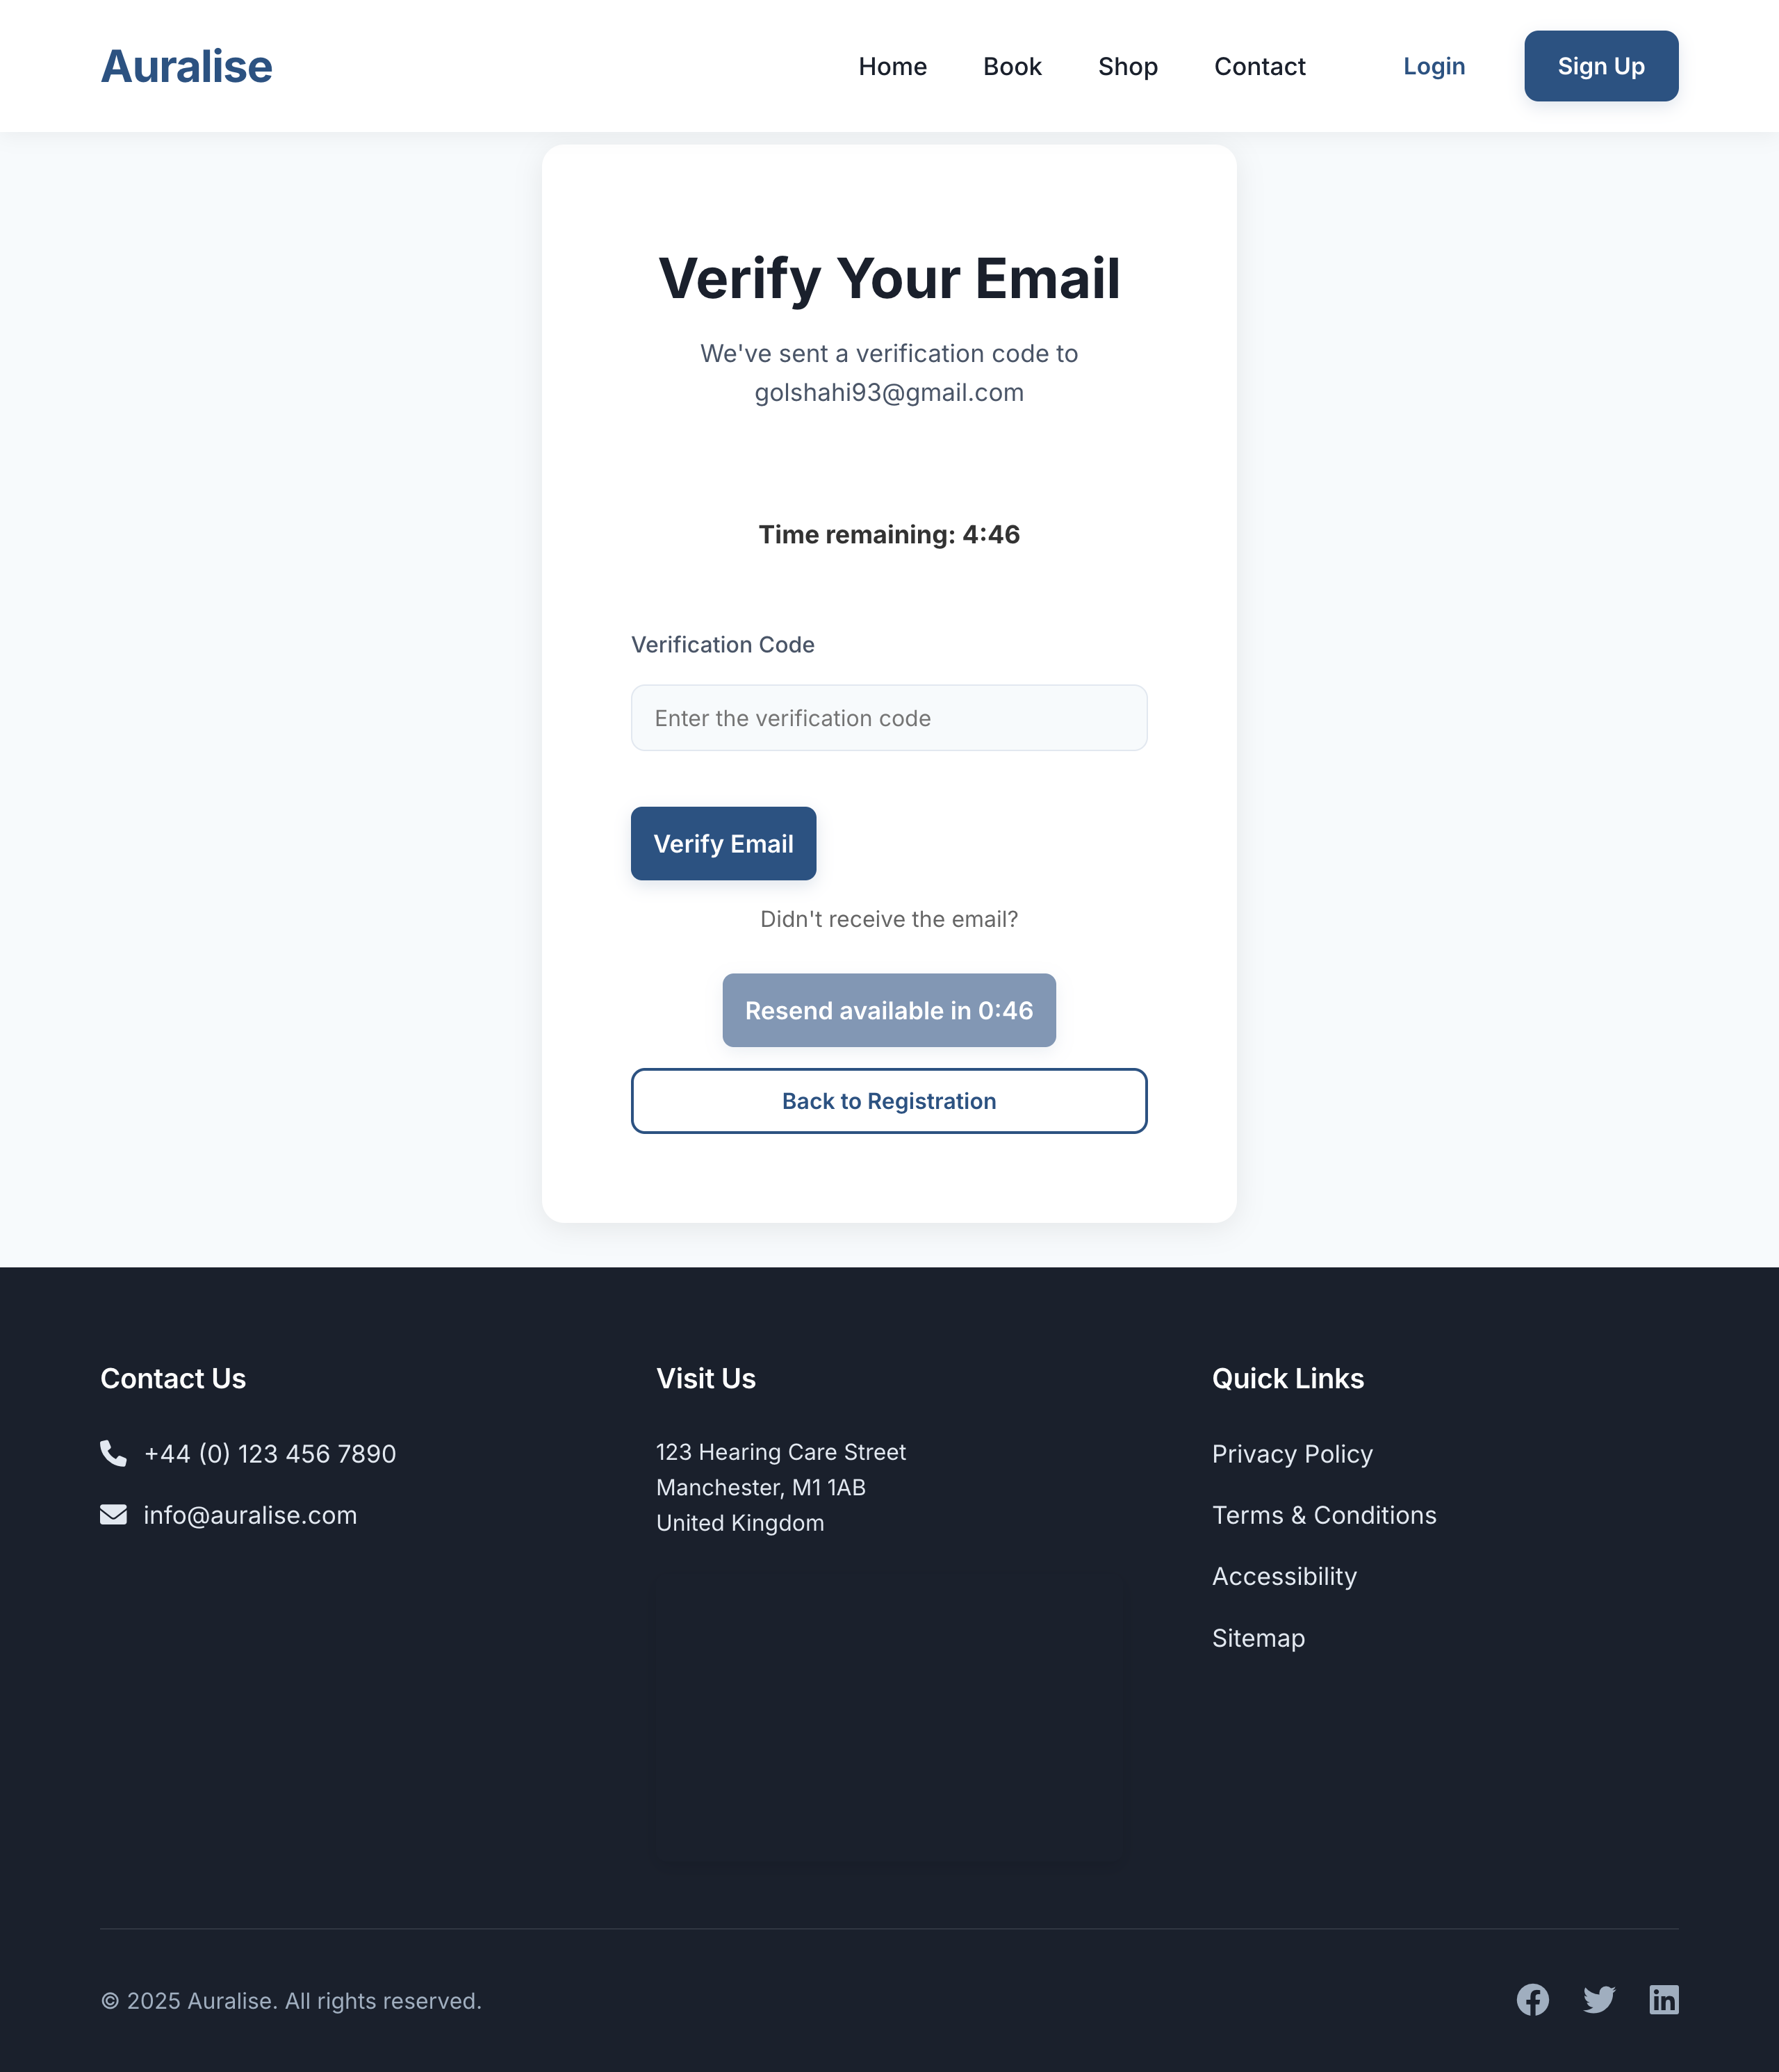
\includegraphics[width=\linewidth, height=0.6\textheight, keepaspectratio]{desktop_otp.png}
    \caption{Desktop OTP}
\end{subfigure}
\caption{OTP Screen (Mobile and Desktop)}
\label{fig:otp_page}
\end{figure}

\begin{figure}[H]
    \centering
    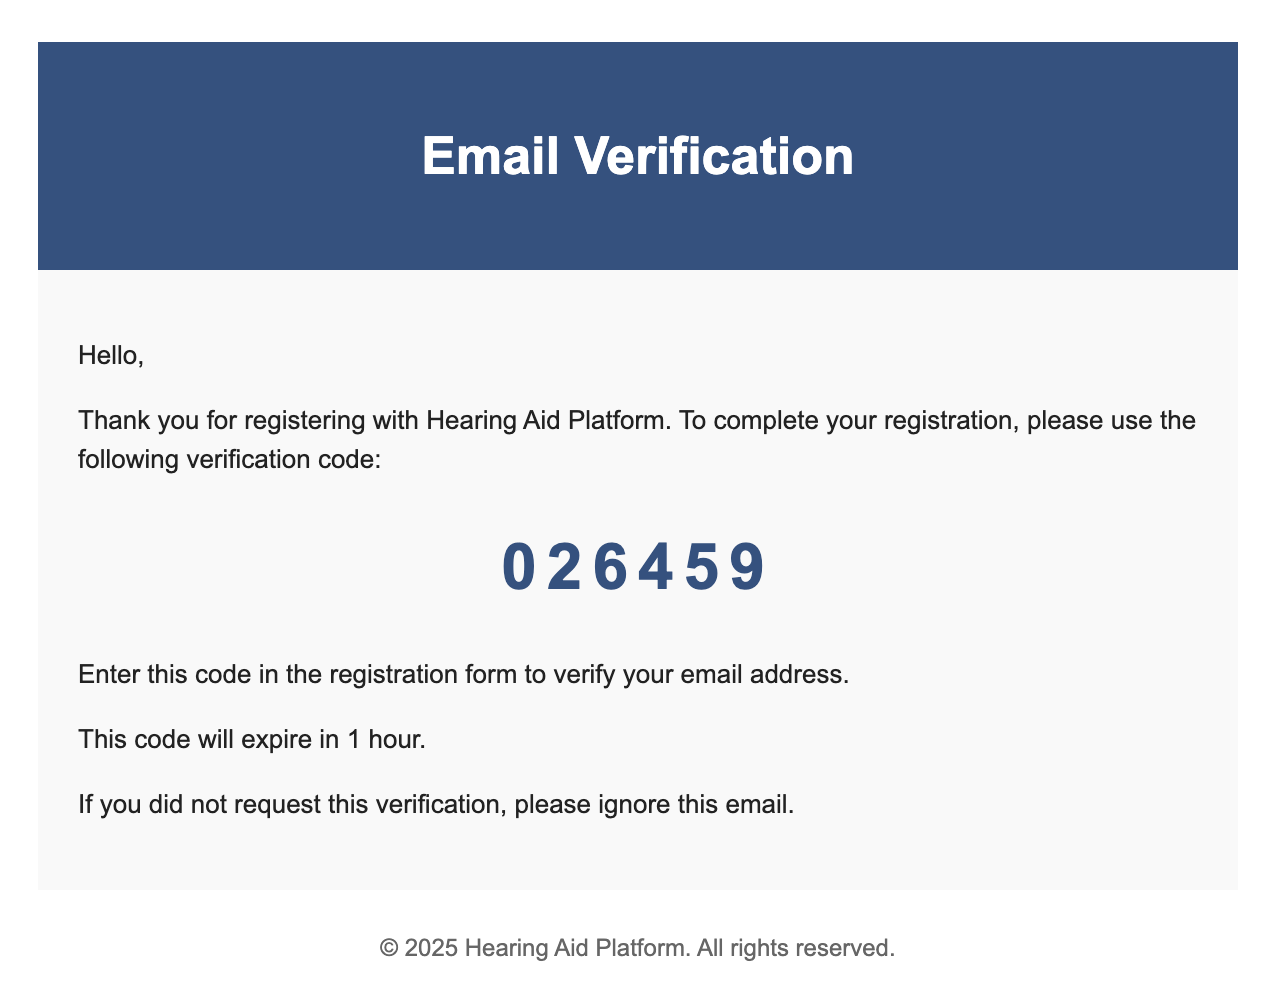
\includegraphics[width=\linewidth, height=0.6\textheight, keepaspectratio]{otp_email.png}
    \caption{OTP Email}
    \label{fig:otp_email}
\end{figure}


The Login Page as shown in Figure~\ref{fig:login_page} allows returning users to access their accounts with email and password authentication. The registration process as shown in Figure~\ref{fig:register_page} includes email verification which can be seen in Figure~\ref{fig:otp_page} to ensure the security of user accounts. During registration, users receive a verification email to be able to successfully register and create an account as can be seen in Figure~\ref{fig:otp_email}, this prevents spam accounts and ensures all accounts on the system are valid.

The platform also supports password recovery through a secure link sent to the user's registered email address. 

\subsubsection{Online Hearing Test}

\begin{figure}[H]
\centering
\begin{subfigure}[b]{0.45\textwidth}
    \centering
    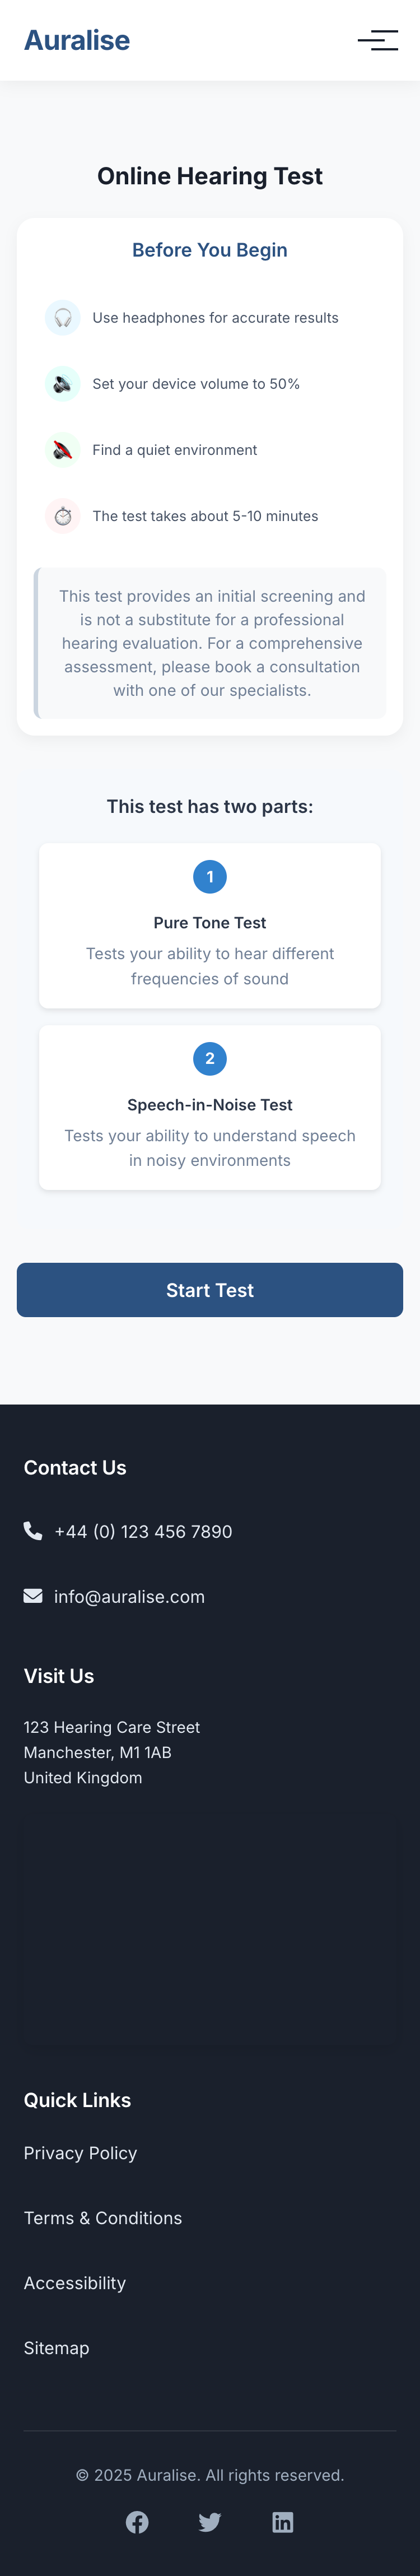
\includegraphics[height=0.5\textheight, keepaspectratio]{mobile_setup.png}
    \subcaption{Mobile Setup}
\end{subfigure}
\hfill
\begin{subfigure}[b]{0.45\textwidth}
    \centering
    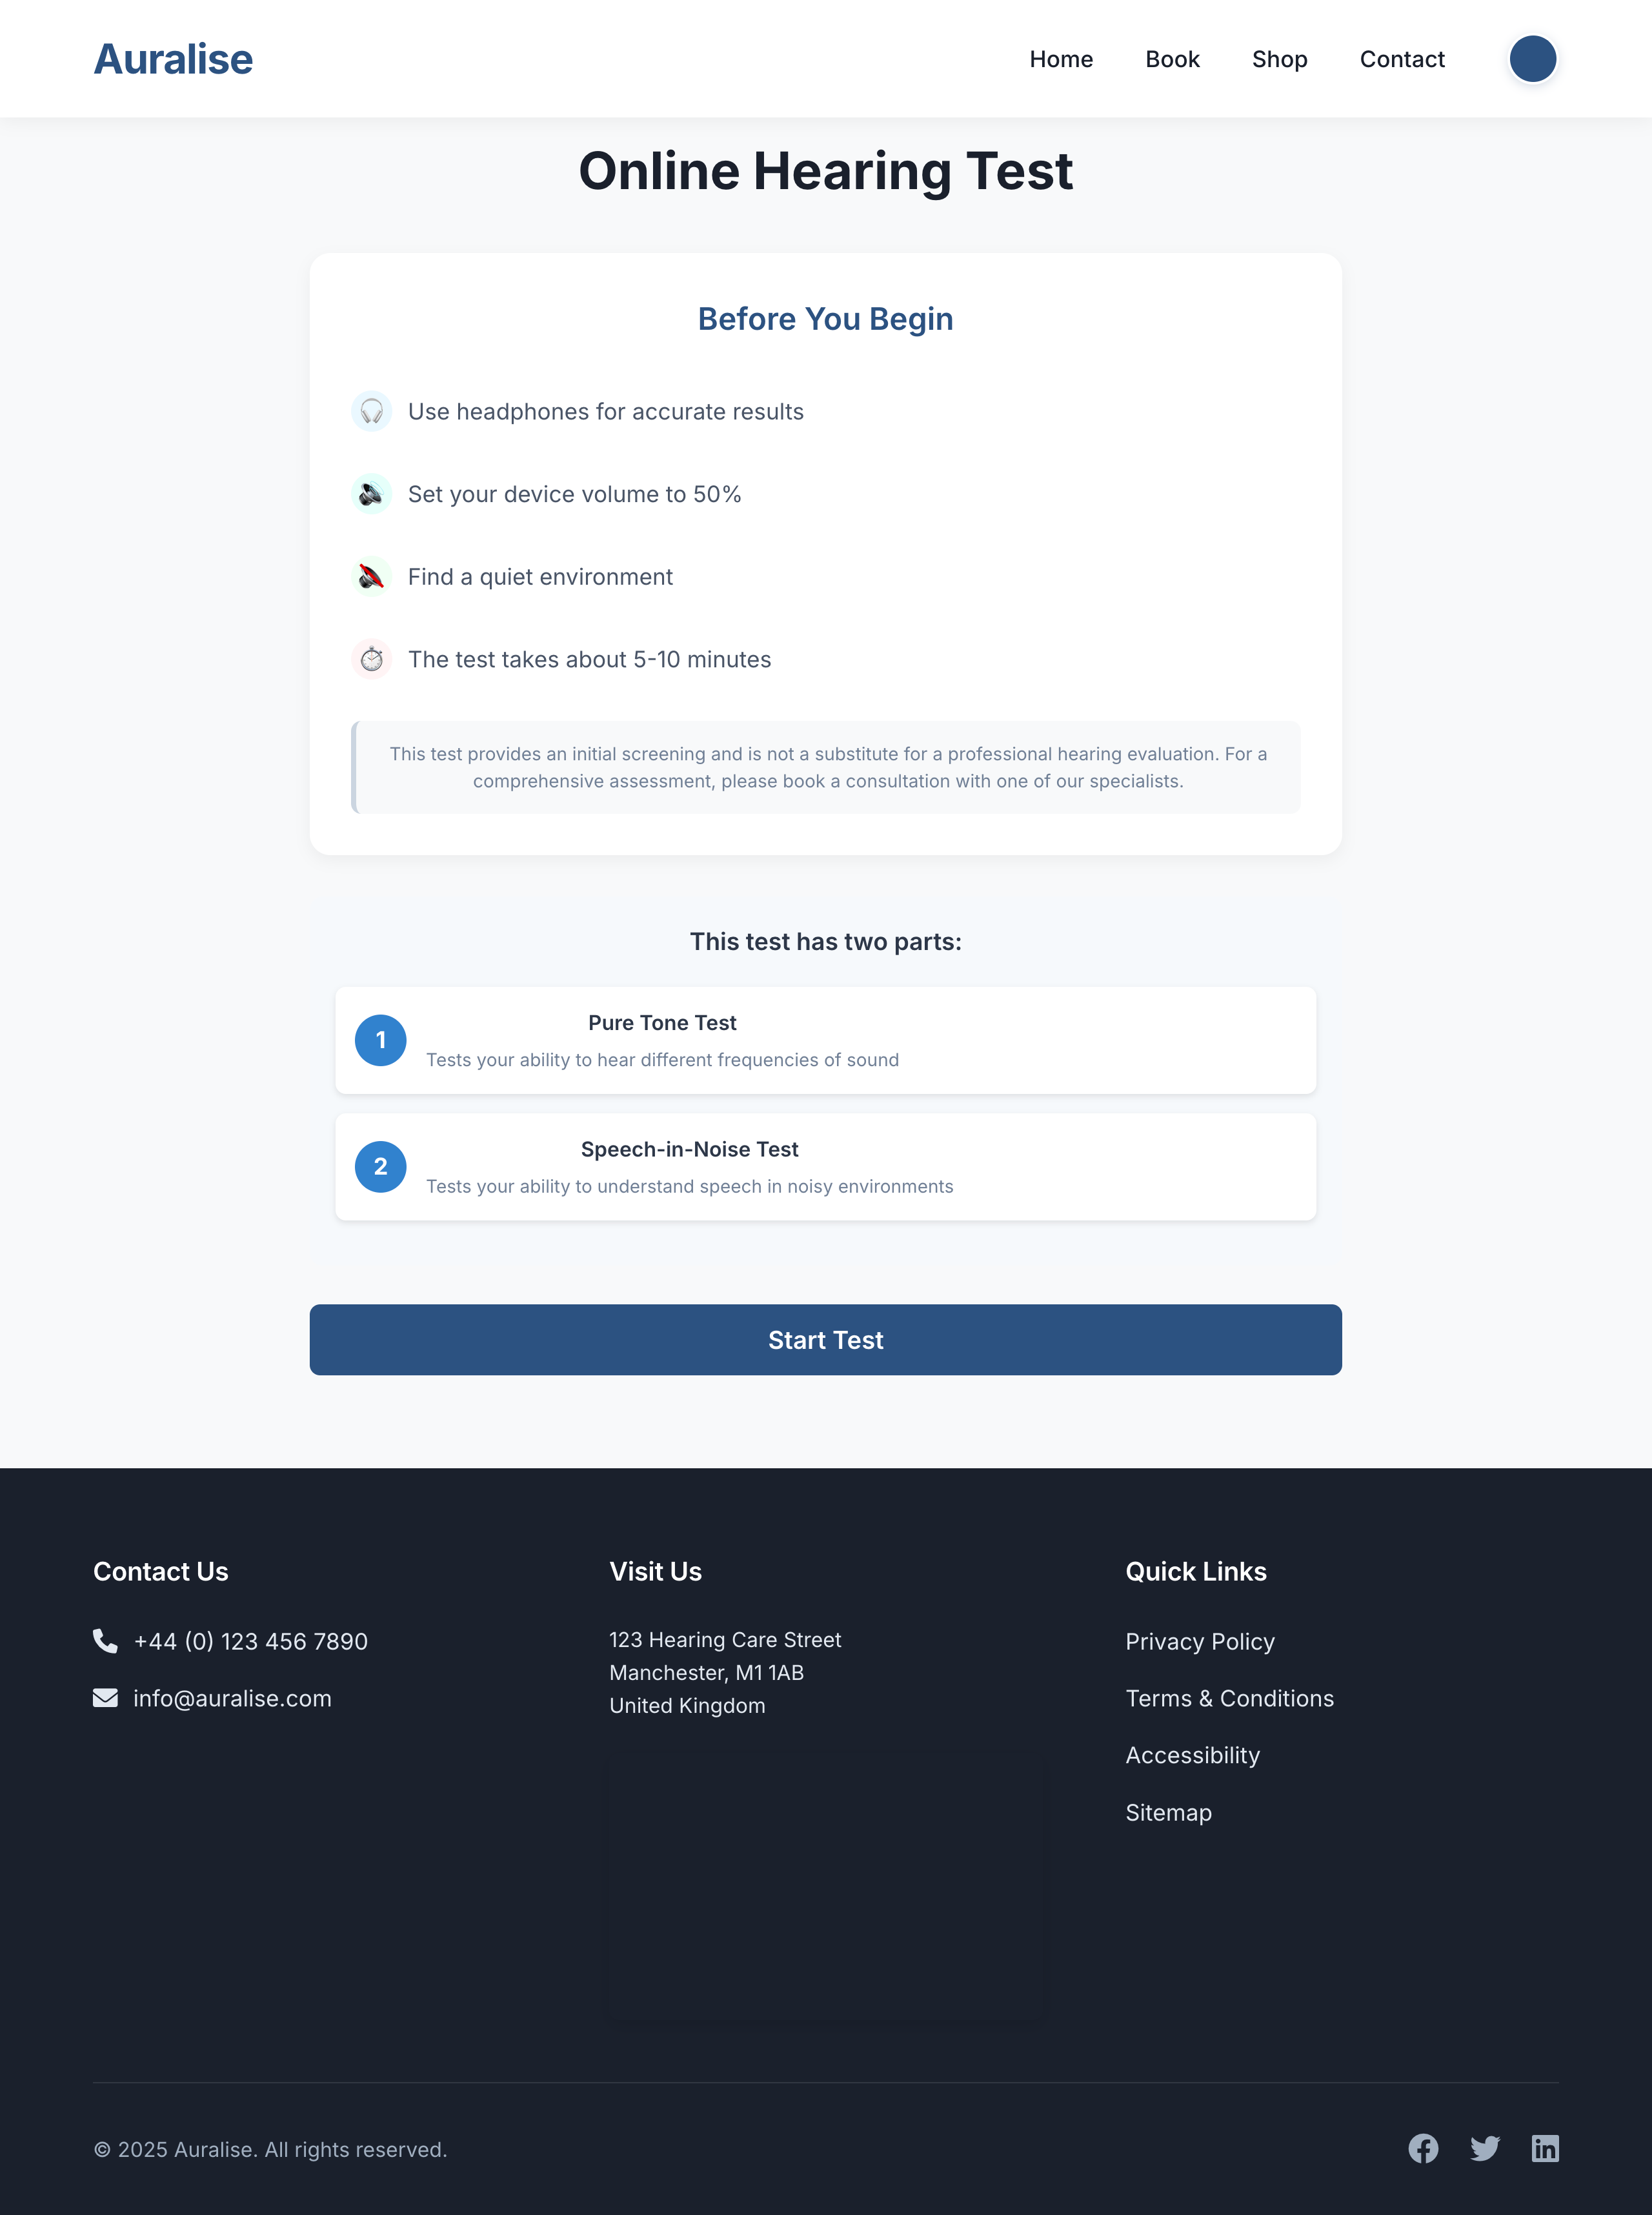
\includegraphics[height=0.4\textheight, keepaspectratio]{desktop_setup.png}
    \subcaption{Desktop Setup}
\end{subfigure}
\caption{Hearing Test Setup Screen (Mobile and Desktop)}
\label{fig:hearing_test_setup}
\end{figure}


\begin{figure}[H]
\centering
\begin{subfigure}[b]{0.45\textwidth}
    \centering
    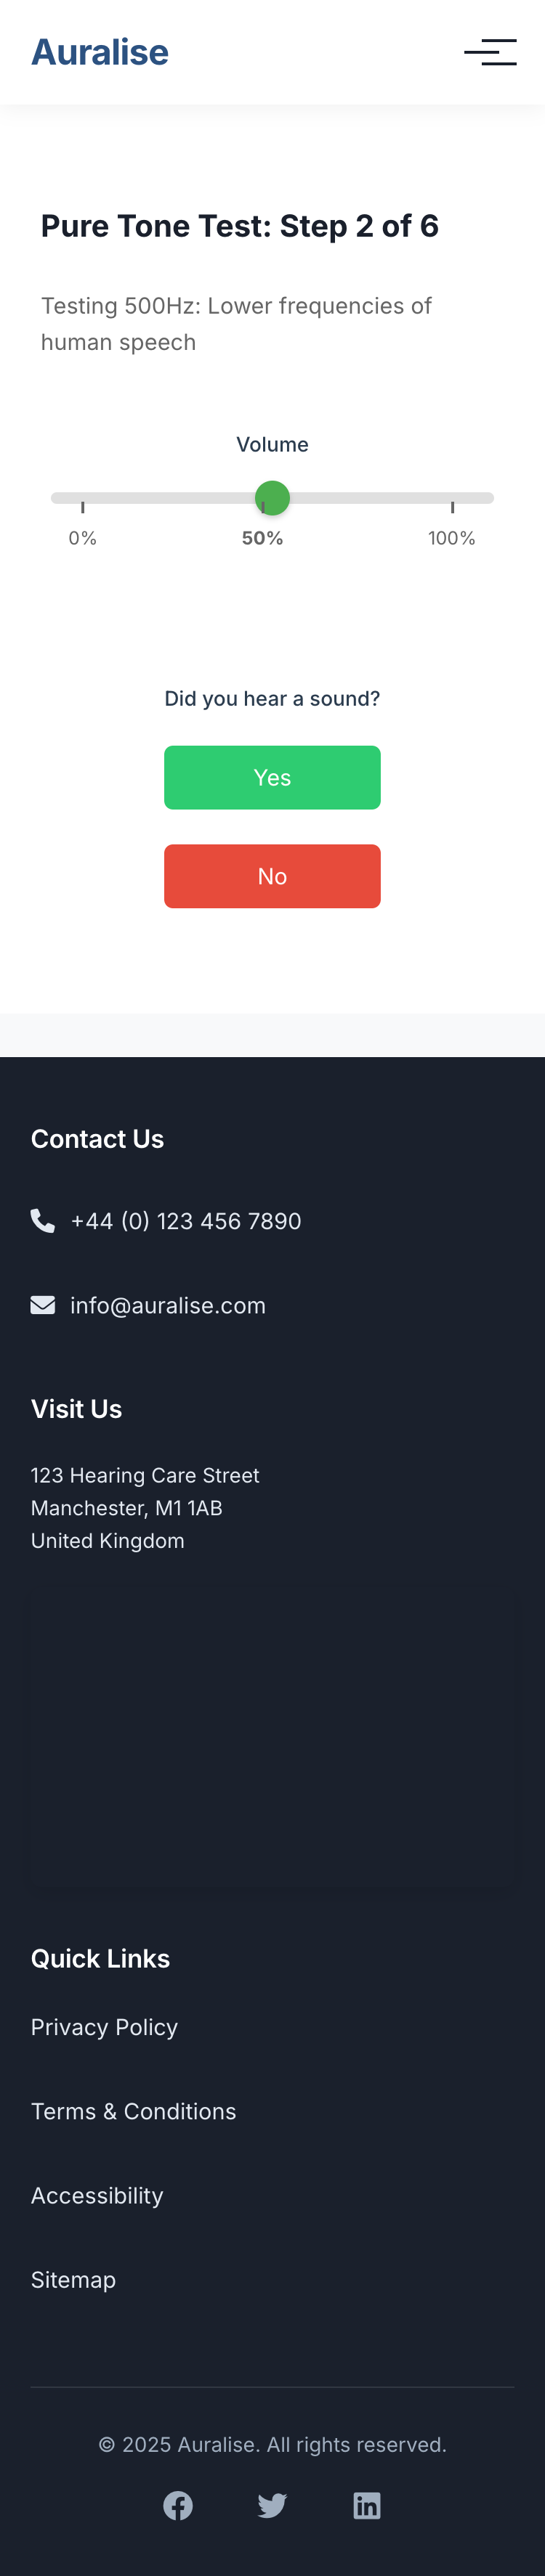
\includegraphics[height=0.5\textheight, keepaspectratio]{mobile_tone_test.png}
    \subcaption{Mobile Tone Test}
\end{subfigure}
\hfill
\begin{subfigure}[b]{0.45\textwidth}
    \centering
    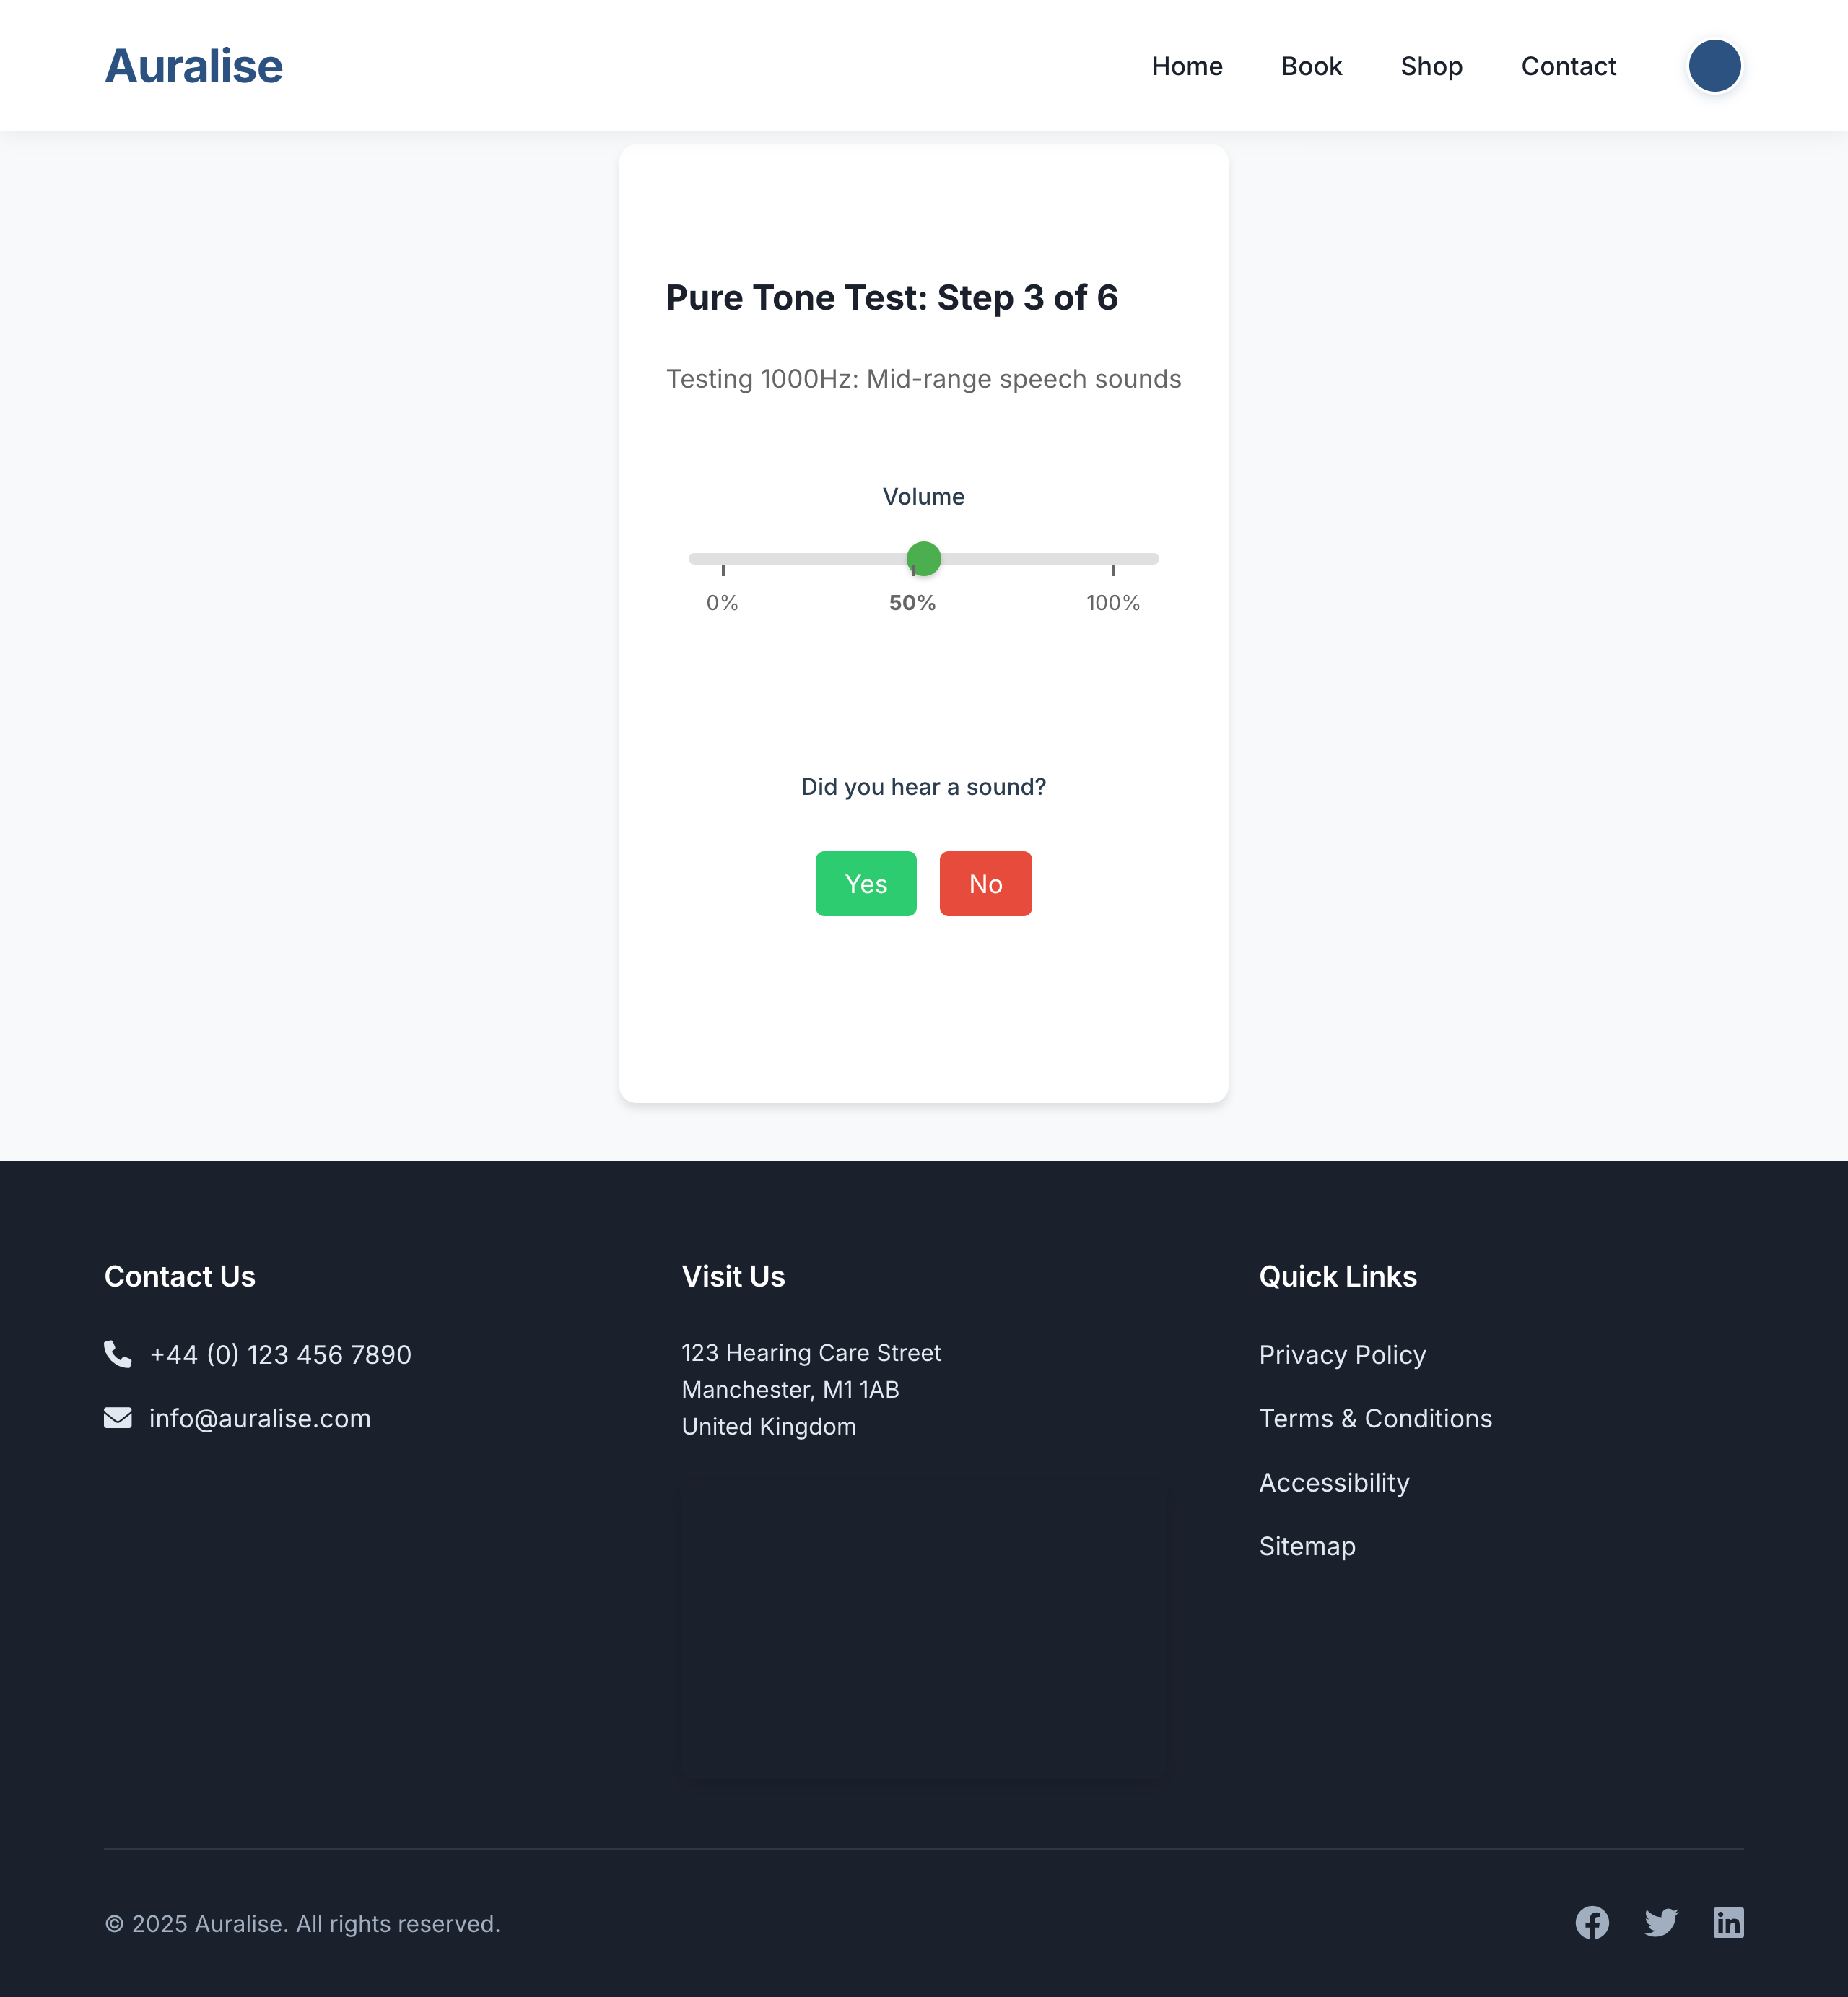
\includegraphics[height=0.3\textheight, keepaspectratio]{desktop_tone_test.png}
    \subcaption{Desktop Tone Test}
\end{subfigure}
\caption{Tone Test Interface (Mobile and Desktop)}
\label{fig:tone_test_interface}
\end{figure}


\begin{figure}[H]
\centering
\begin{subfigure}[b]{0.45\textwidth}
    \centering
    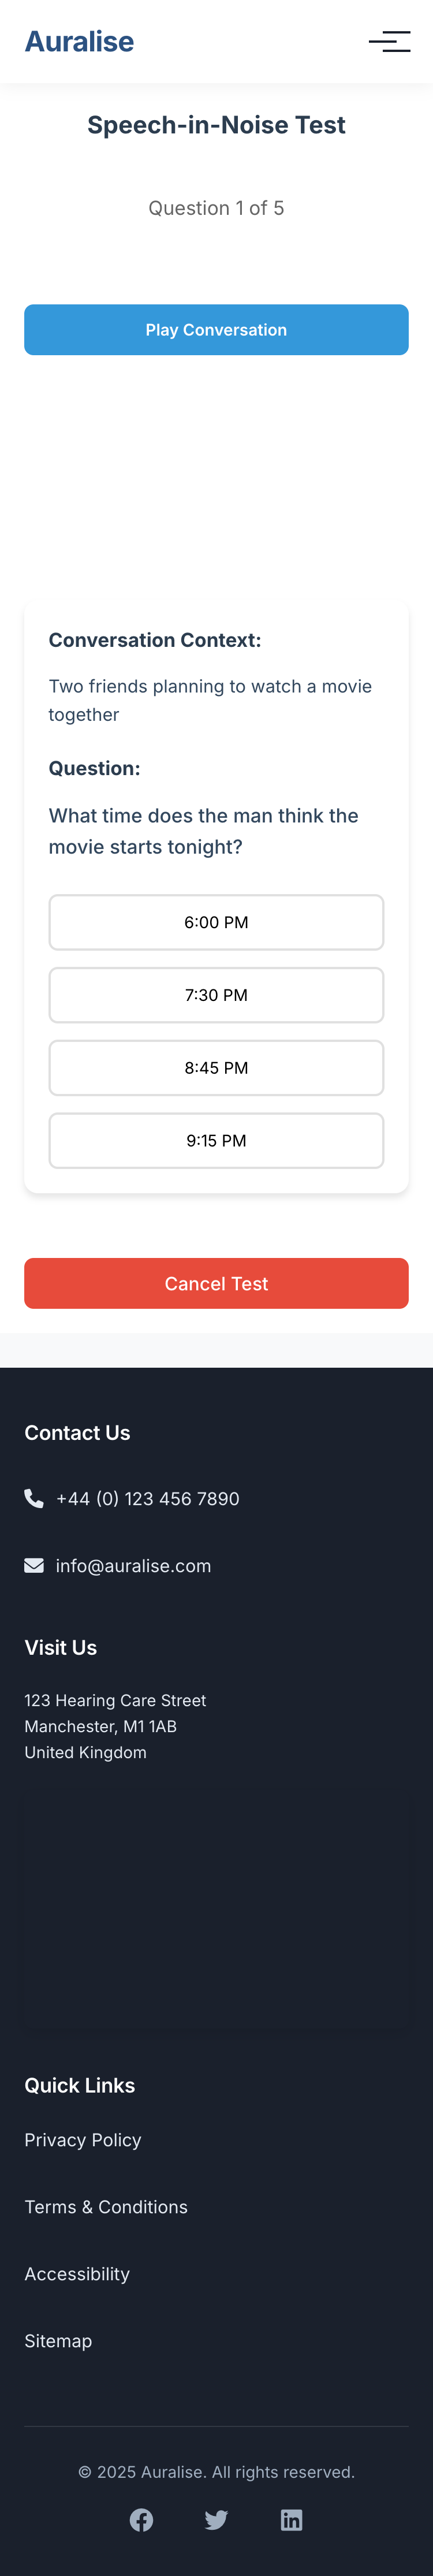
\includegraphics[height=0.5\textheight, keepaspectratio]{mobile_speech_noise.png}
    \subcaption{Mobile Speech-in-Noise}
\end{subfigure}
\hfill
\begin{subfigure}[b]{0.45\textwidth}
    \centering
    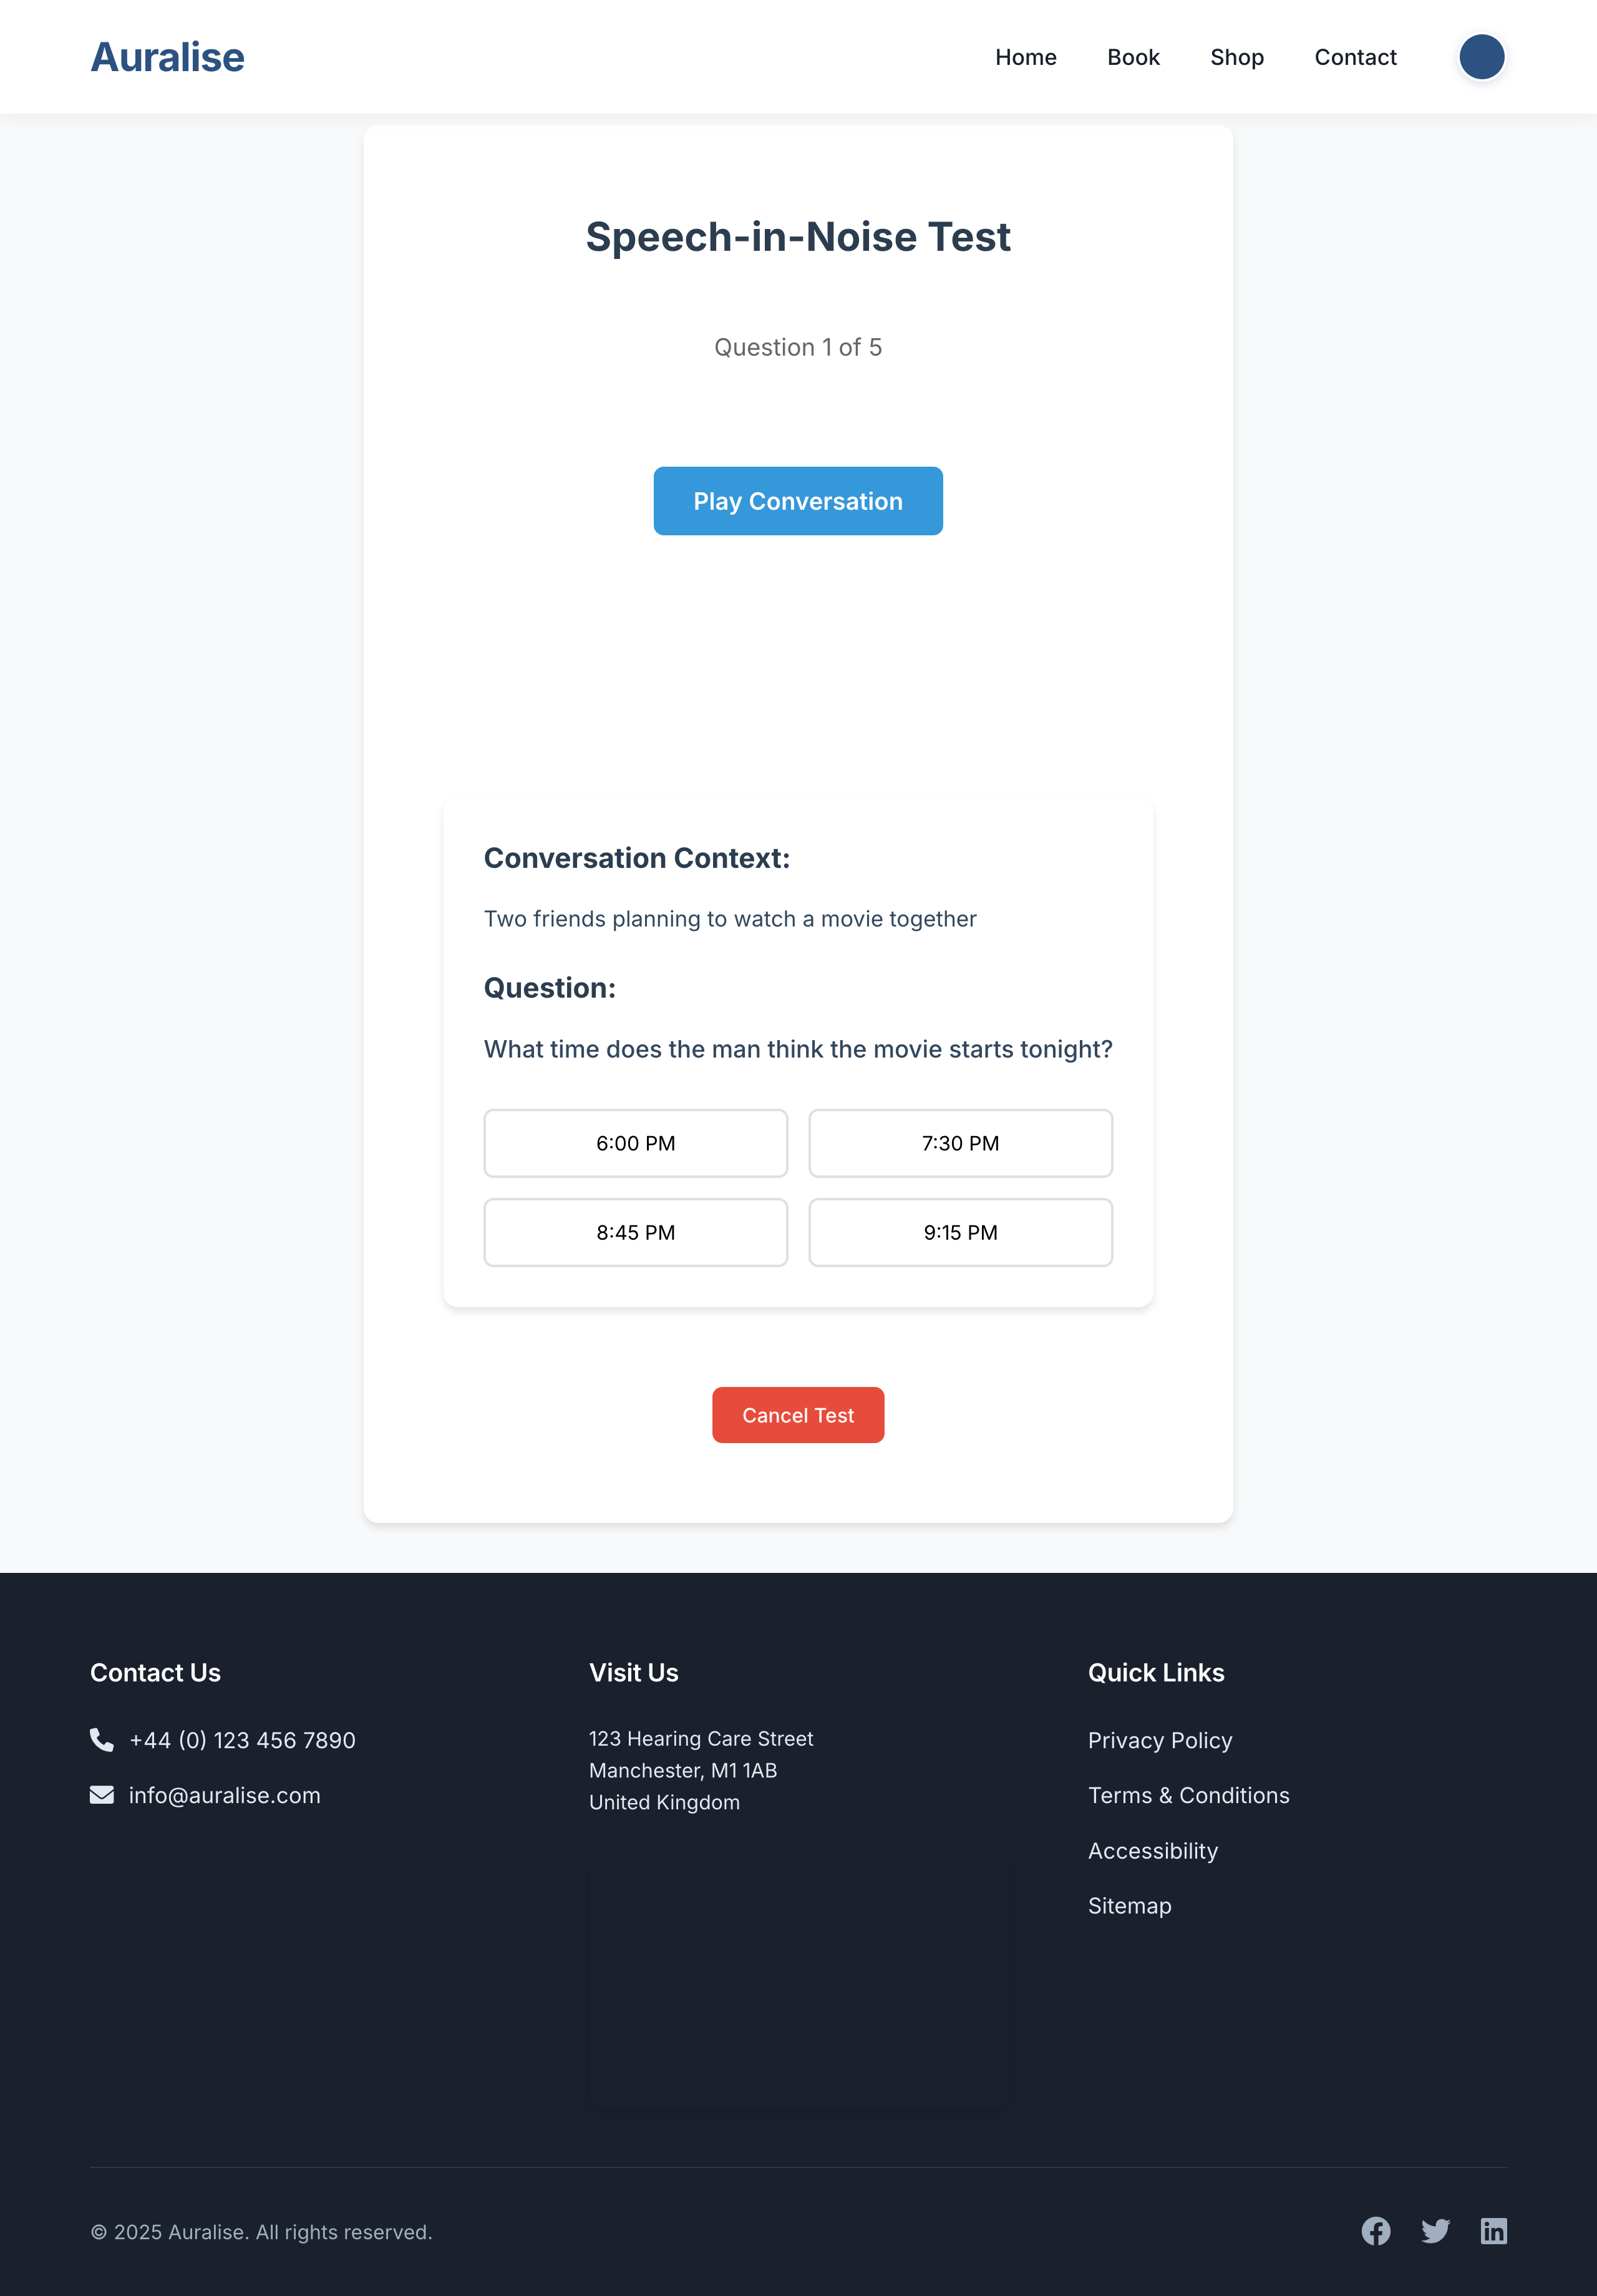
\includegraphics[height=0.4\textheight, keepaspectratio]{desktop_speech_noise.png}
    \subcaption{Desktop Speech-in-Noise}
\end{subfigure}
\caption{Speech-in-Noise Test (Mobile and Desktop)}
\label{fig:speech_in_noise_test}
\end{figure}


\begin{figure}[H]
\centering
\begin{subfigure}[b]{0.45\textwidth}
    \centering
    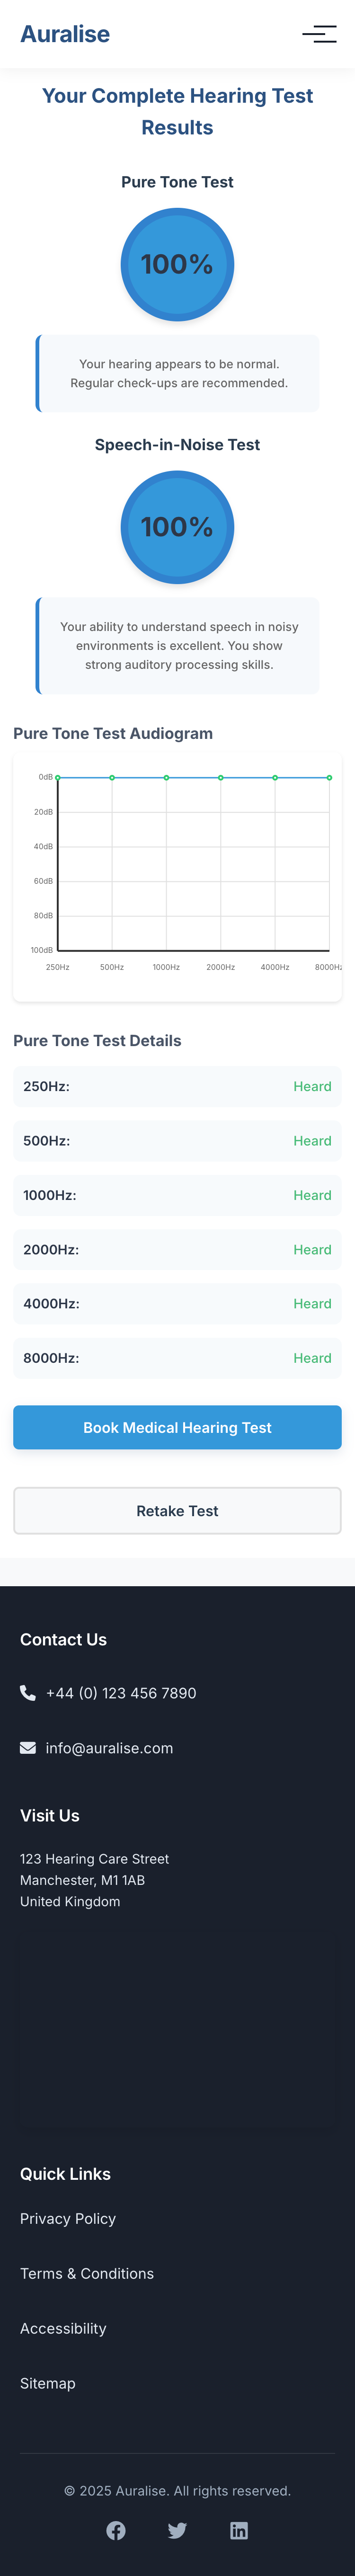
\includegraphics[height=0.5\textheight, keepaspectratio]{mobile_test_results.png}
    \subcaption{Mobile Results}
\end{subfigure}
\hfill
\begin{subfigure}[b]{0.45\textwidth}
    \centering
    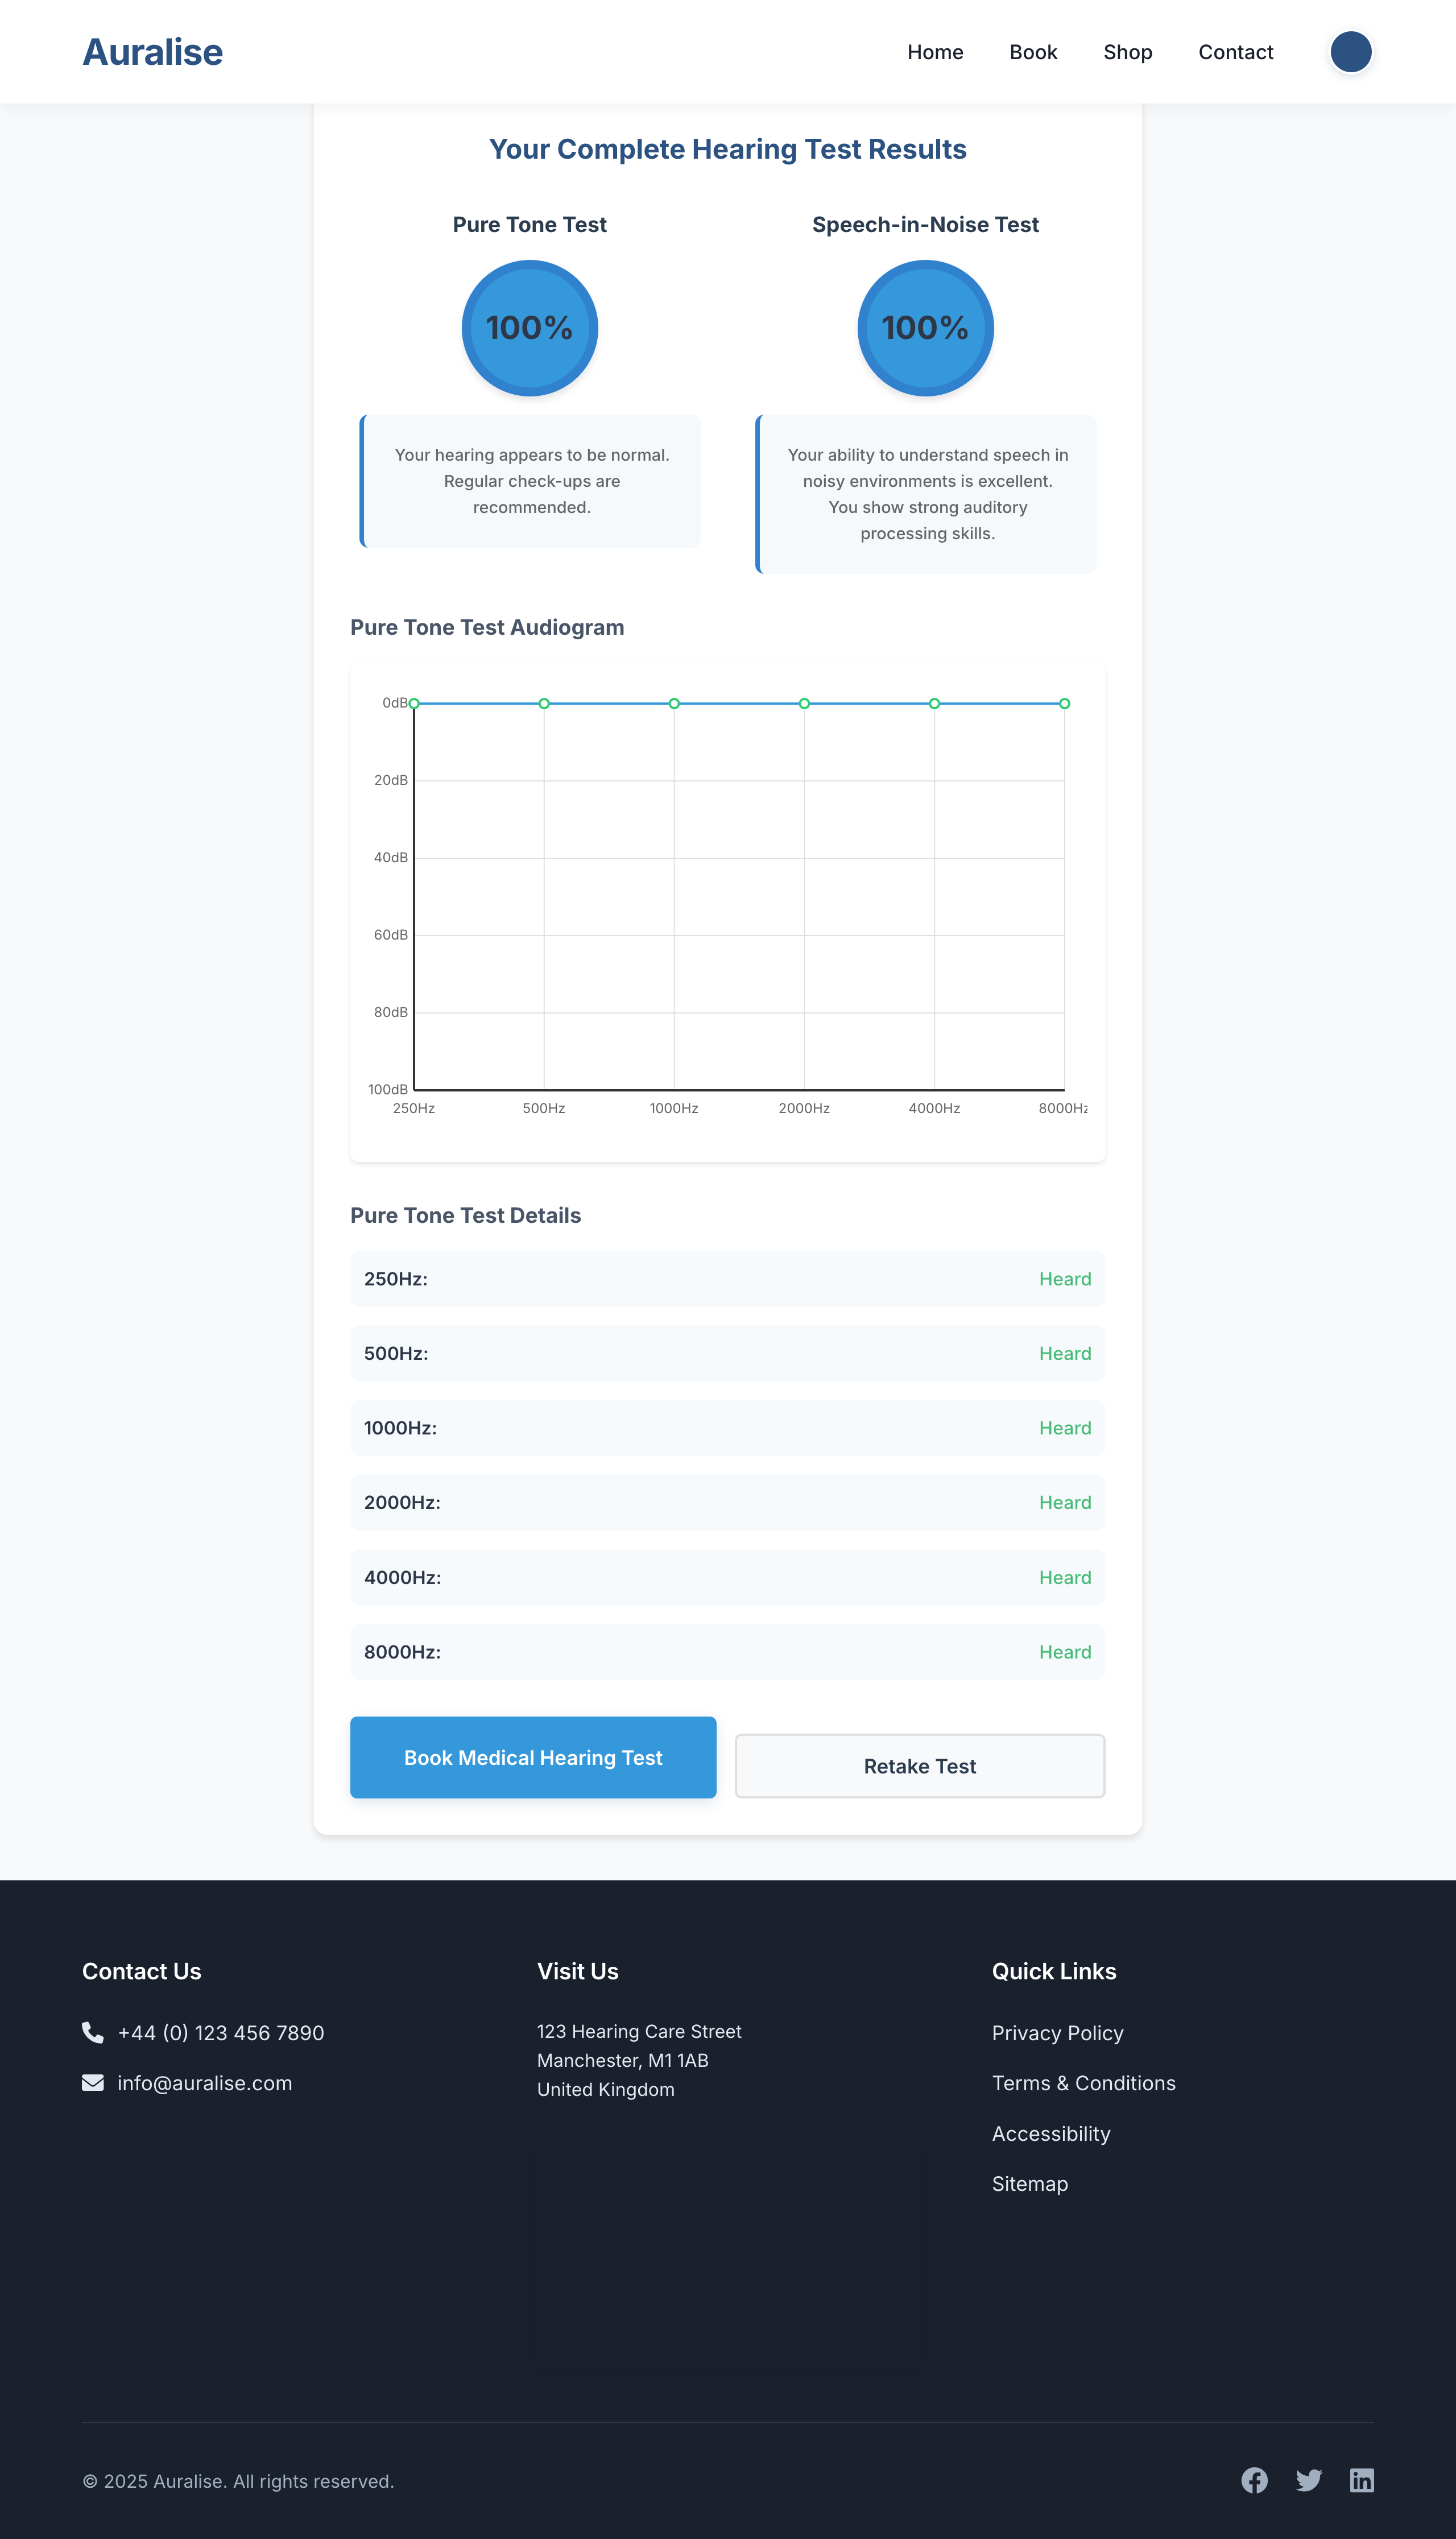
\includegraphics[height=0.5\textheight, keepaspectratio]{desktop_test_results.png}
    \subcaption{Desktop Results}
\end{subfigure}
\caption{Hearing Test Results (Mobile and Desktop)}
\label{fig:hearing_test_results}
\end{figure}


The Online Hearing Test is a cornerstone feature of the platform, offering users a preliminary assessment of their hearing capabilities. As shown in Figure\ref{fig:hearing_test_setup}, the test starts with an environment check that detects background noise levels and whether headphones are being used, ensuring optimal testing conditions

The test consists of three parts:
\begin{enumerate}
    \item Tone Test: As shown in Figure~\ref{fig:tone_test_interface}, users listen for pure tones at different frequencies (250Hz to 8000Hz) at random intervals (to prevent placebo effect) \cite{interacoustics_pure_tone_2024} and indicate when they can hear them. The application progressively adjusts volume levels to determine hearing thresholds.
    \item Speech-in-Noise Test: As shown in Figure~\ref{fig:speech_in_noise_test}, users listen to spoken words or sentences with varying levels of background noise and must identify what was said, simulating real-world listening environments \cite{billings_speech-in-noise_2024}.
\end{enumerate}

Results are presented as an audiogram graph showing hearing sensitivity across different frequencies, along with a personalized recommendation as reflected in Figure~\ref{fig:hearing_test_results}. Users can save their results to their profile and share them with audiologists during consultations.

\subsubsection{Product Browsing and AR Try-On}


\begin{figure}[H]
\centering
\begin{subfigure}[b]{0.45\textwidth}
    \centering
    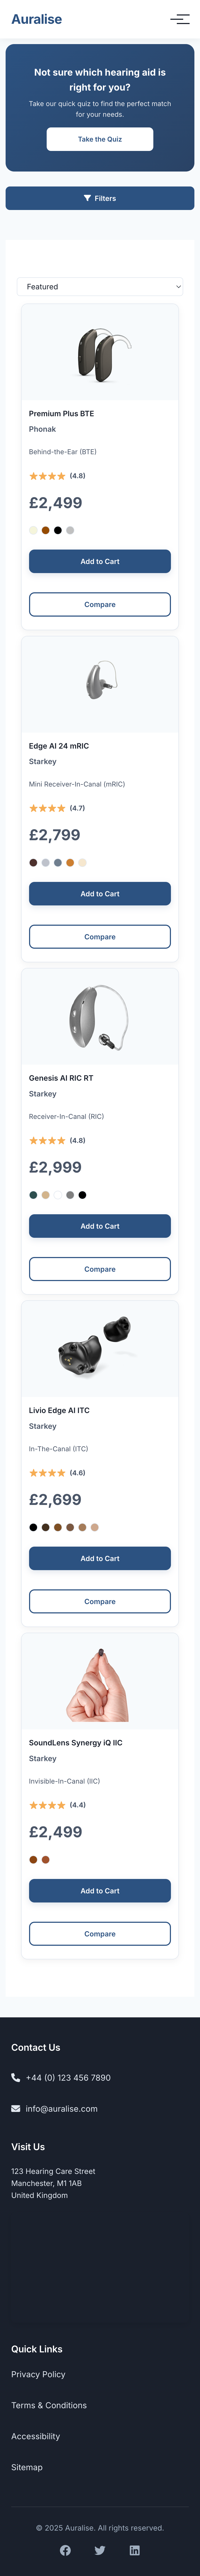
\includegraphics[height=0.5\textheight, keepaspectratio]{mobile_shop.png}
    \subcaption{Mobile Shop Page}
\end{subfigure}
\hfill
\begin{subfigure}[b]{0.45\textwidth}
    \centering
    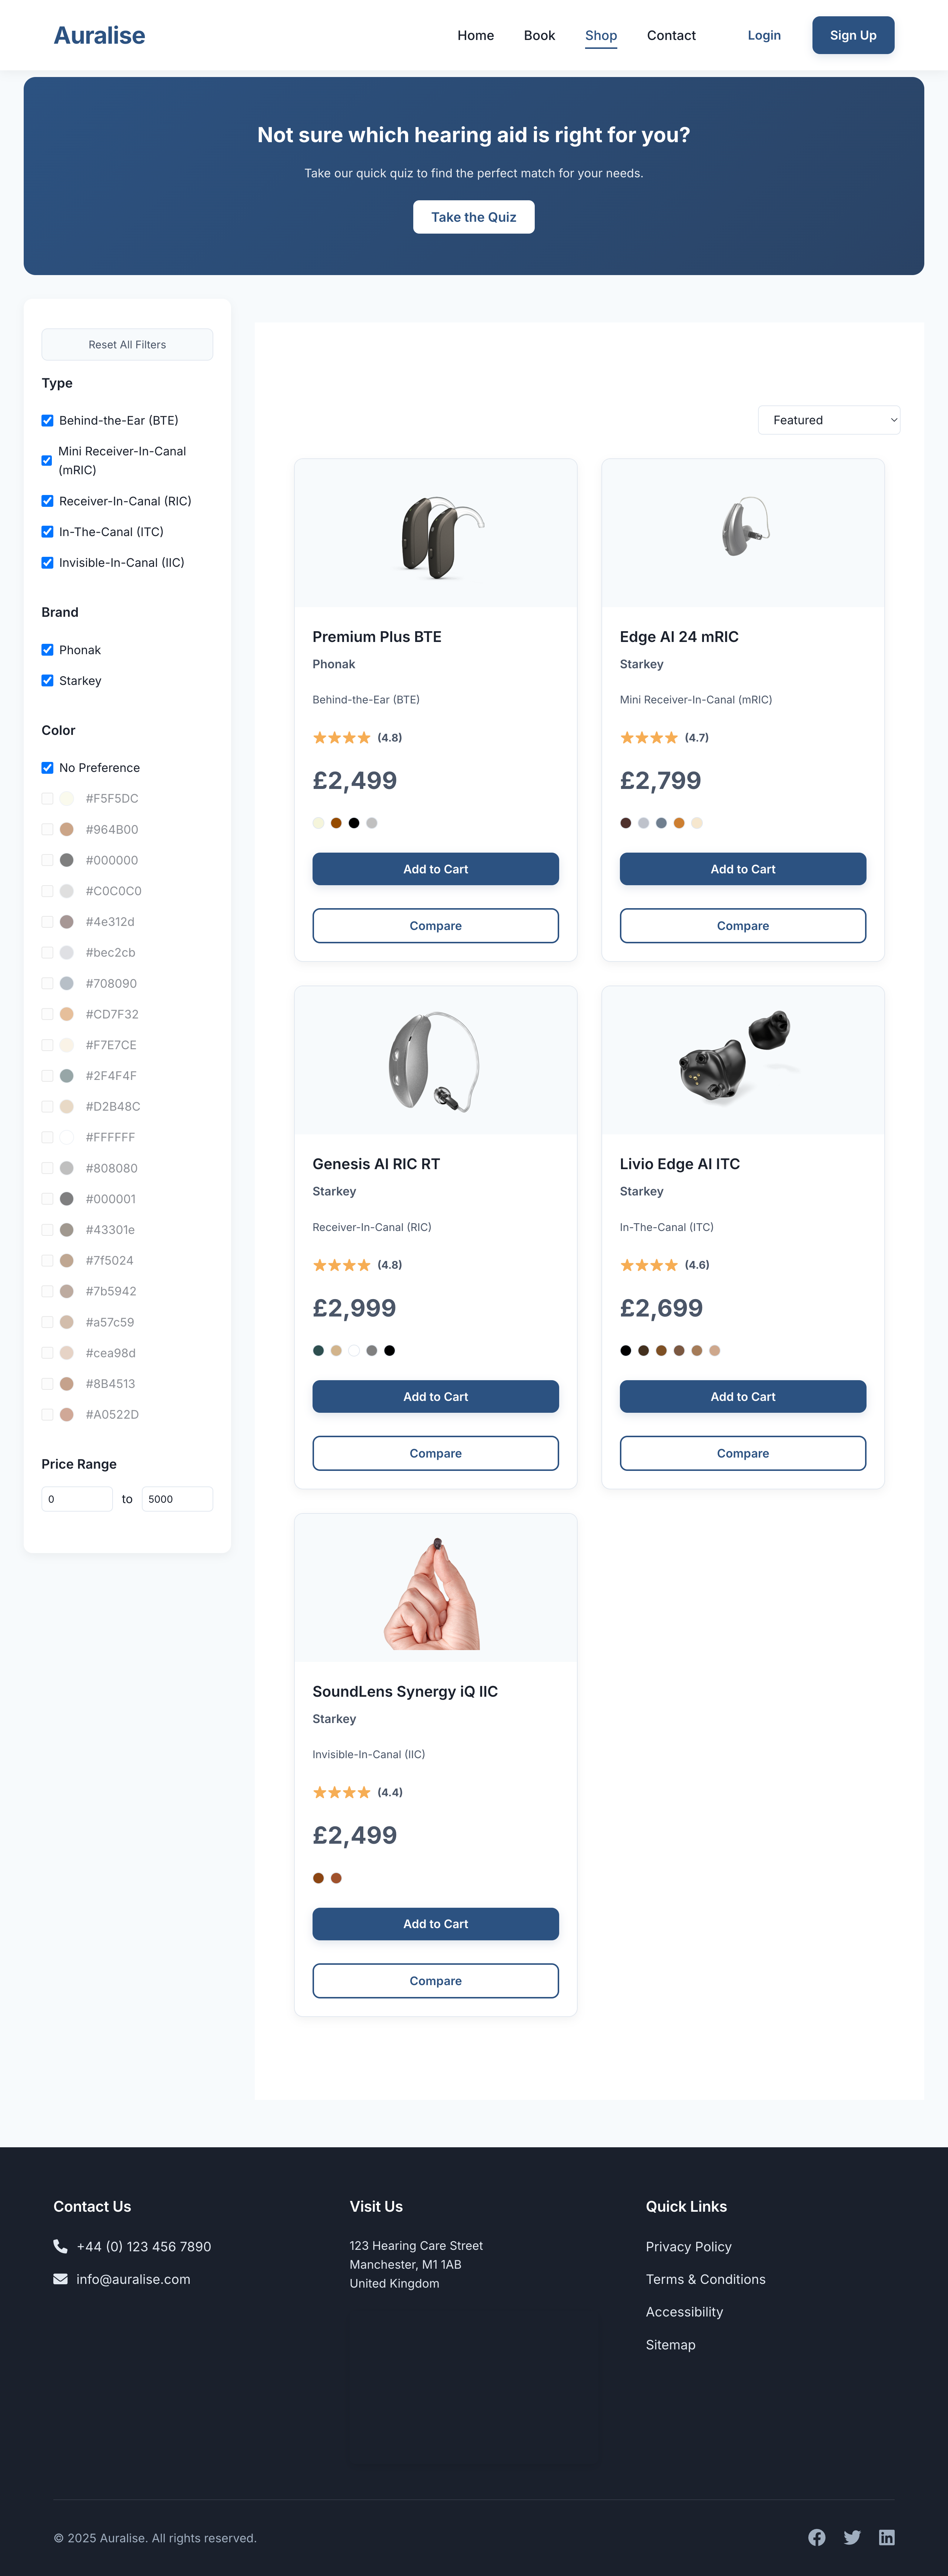
\includegraphics[height=0.5\textheight, keepaspectratio]{desktop_shop.png}
    \subcaption{Desktop Shop Page}
\end{subfigure}
\caption{Shop Page (Mobile and Desktop)}
\label{fig:shop_page}
\end{figure}


\begin{figure}[H]
\centering
\begin{subfigure}[b]{0.45\textwidth}
    \centering
    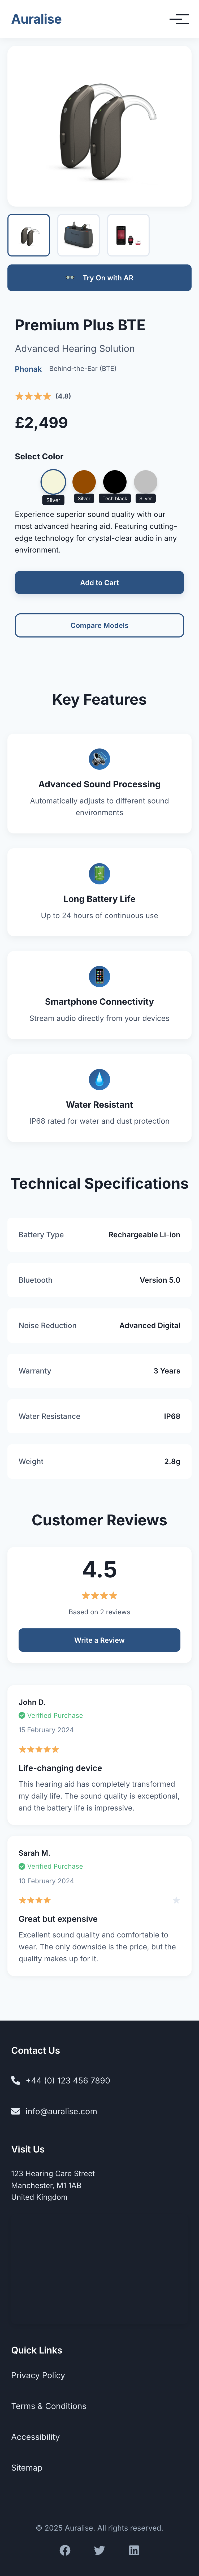
\includegraphics[height=0.5\textheight, keepaspectratio]{mobile_product_detail.png}
    \subcaption{Mobile Product Detail Page}
\end{subfigure}
\hfill
\begin{subfigure}[b]{0.45\textwidth}
    \centering
    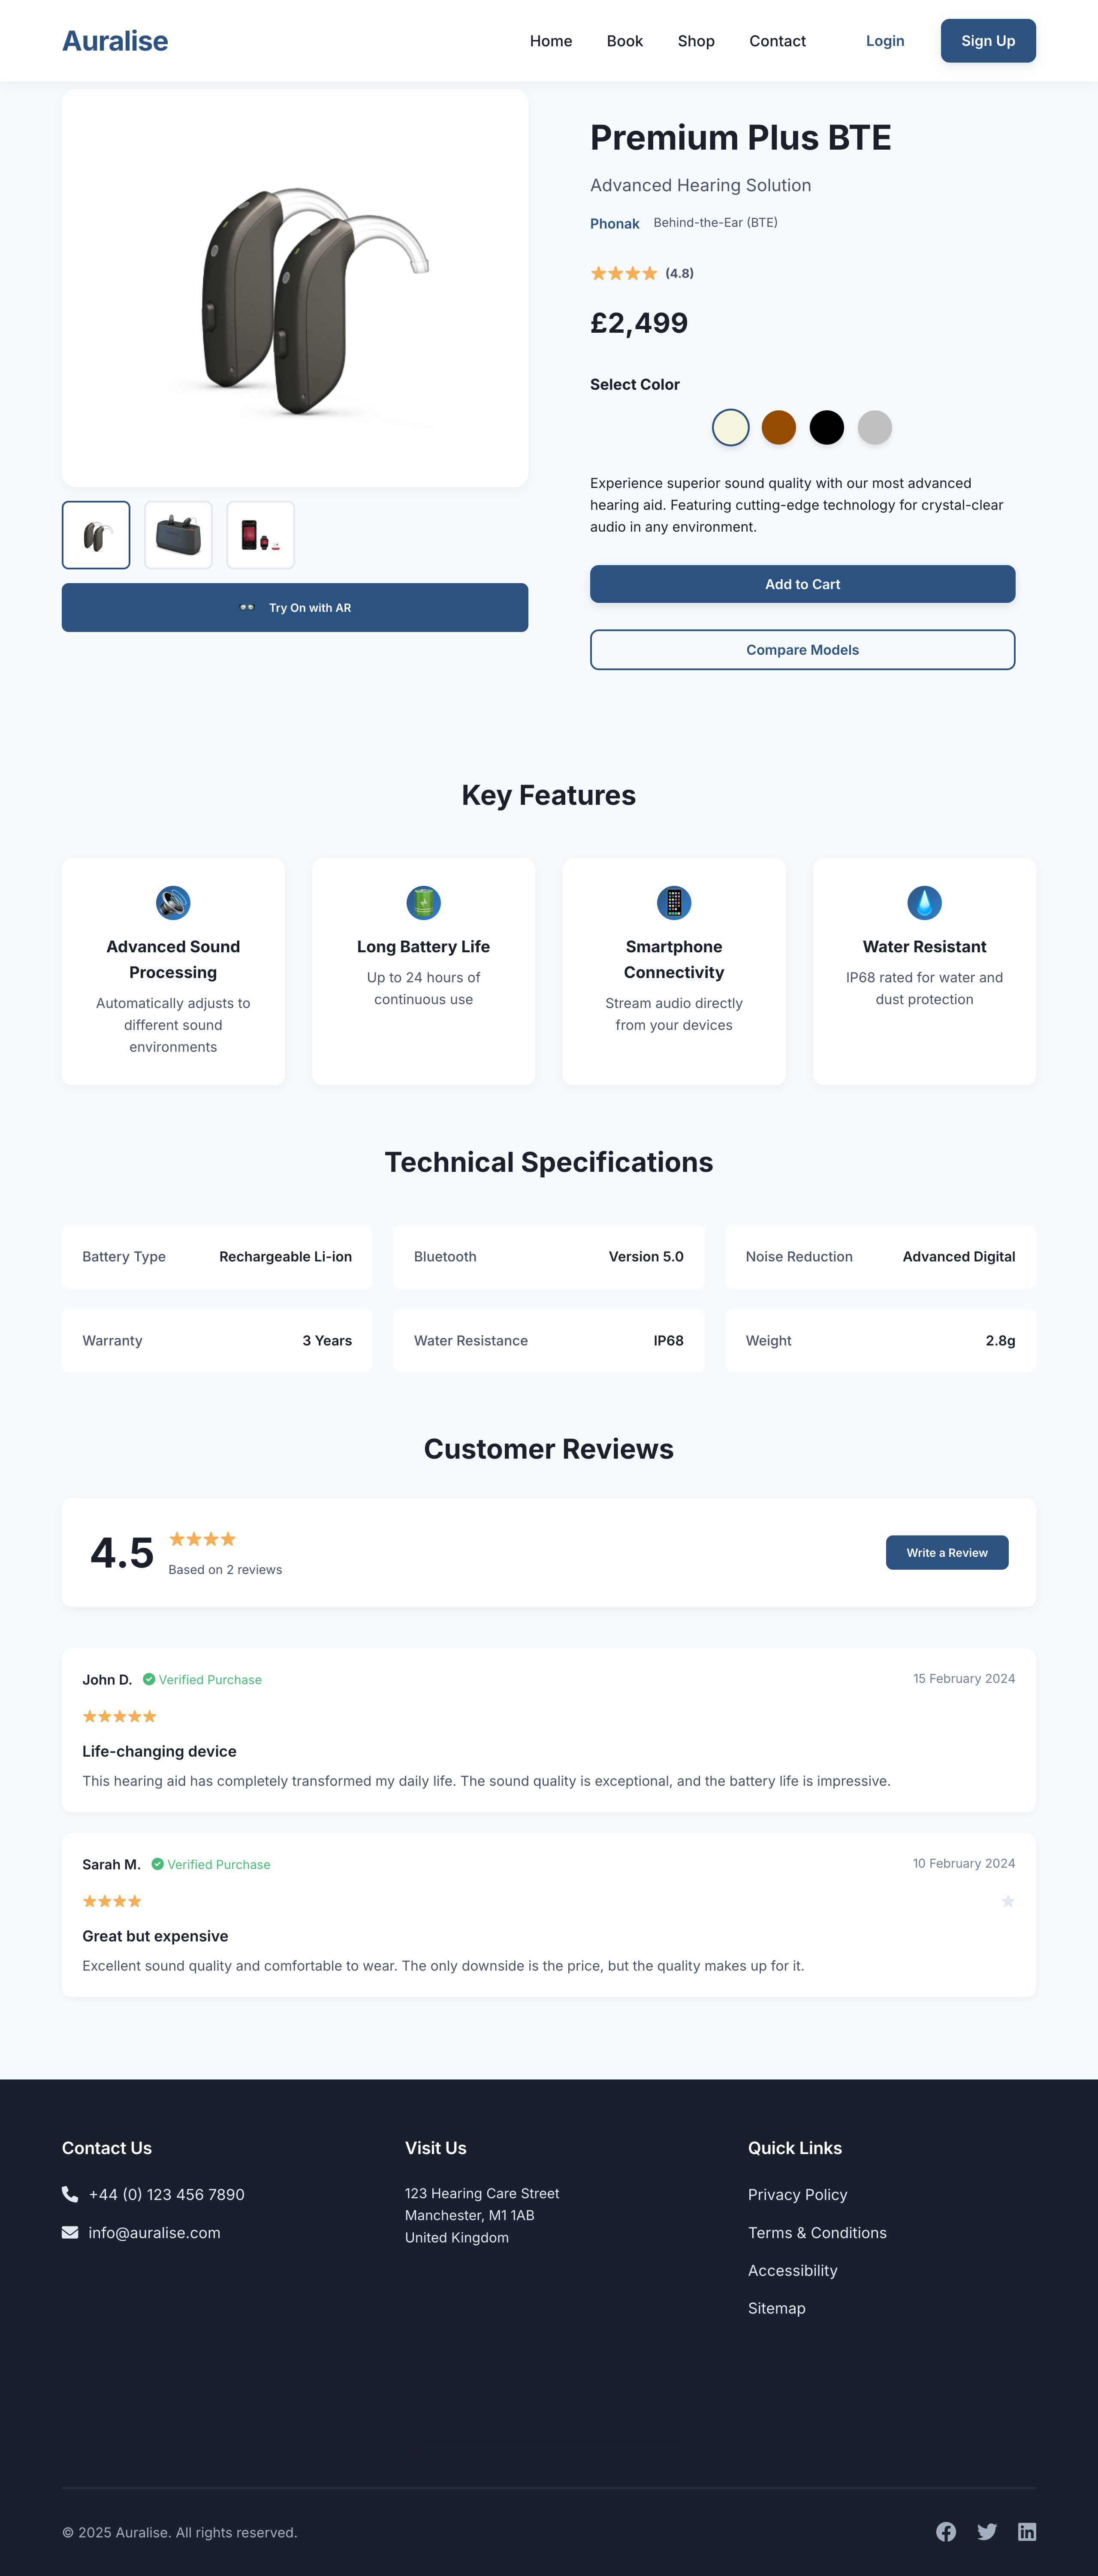
\includegraphics[height=0.5\textheight, keepaspectratio]{desktop_product_detail.png}
    \subcaption{Desktop Product Detail Page}
\end{subfigure}
\caption{Product Detail Page (Mobile and Desktop)}
\label{fig:product_detail_page}
\end{figure}


\begin{figure}[H]
\centering
\begin{subfigure}[b]{0.45\textwidth}
    \centering
    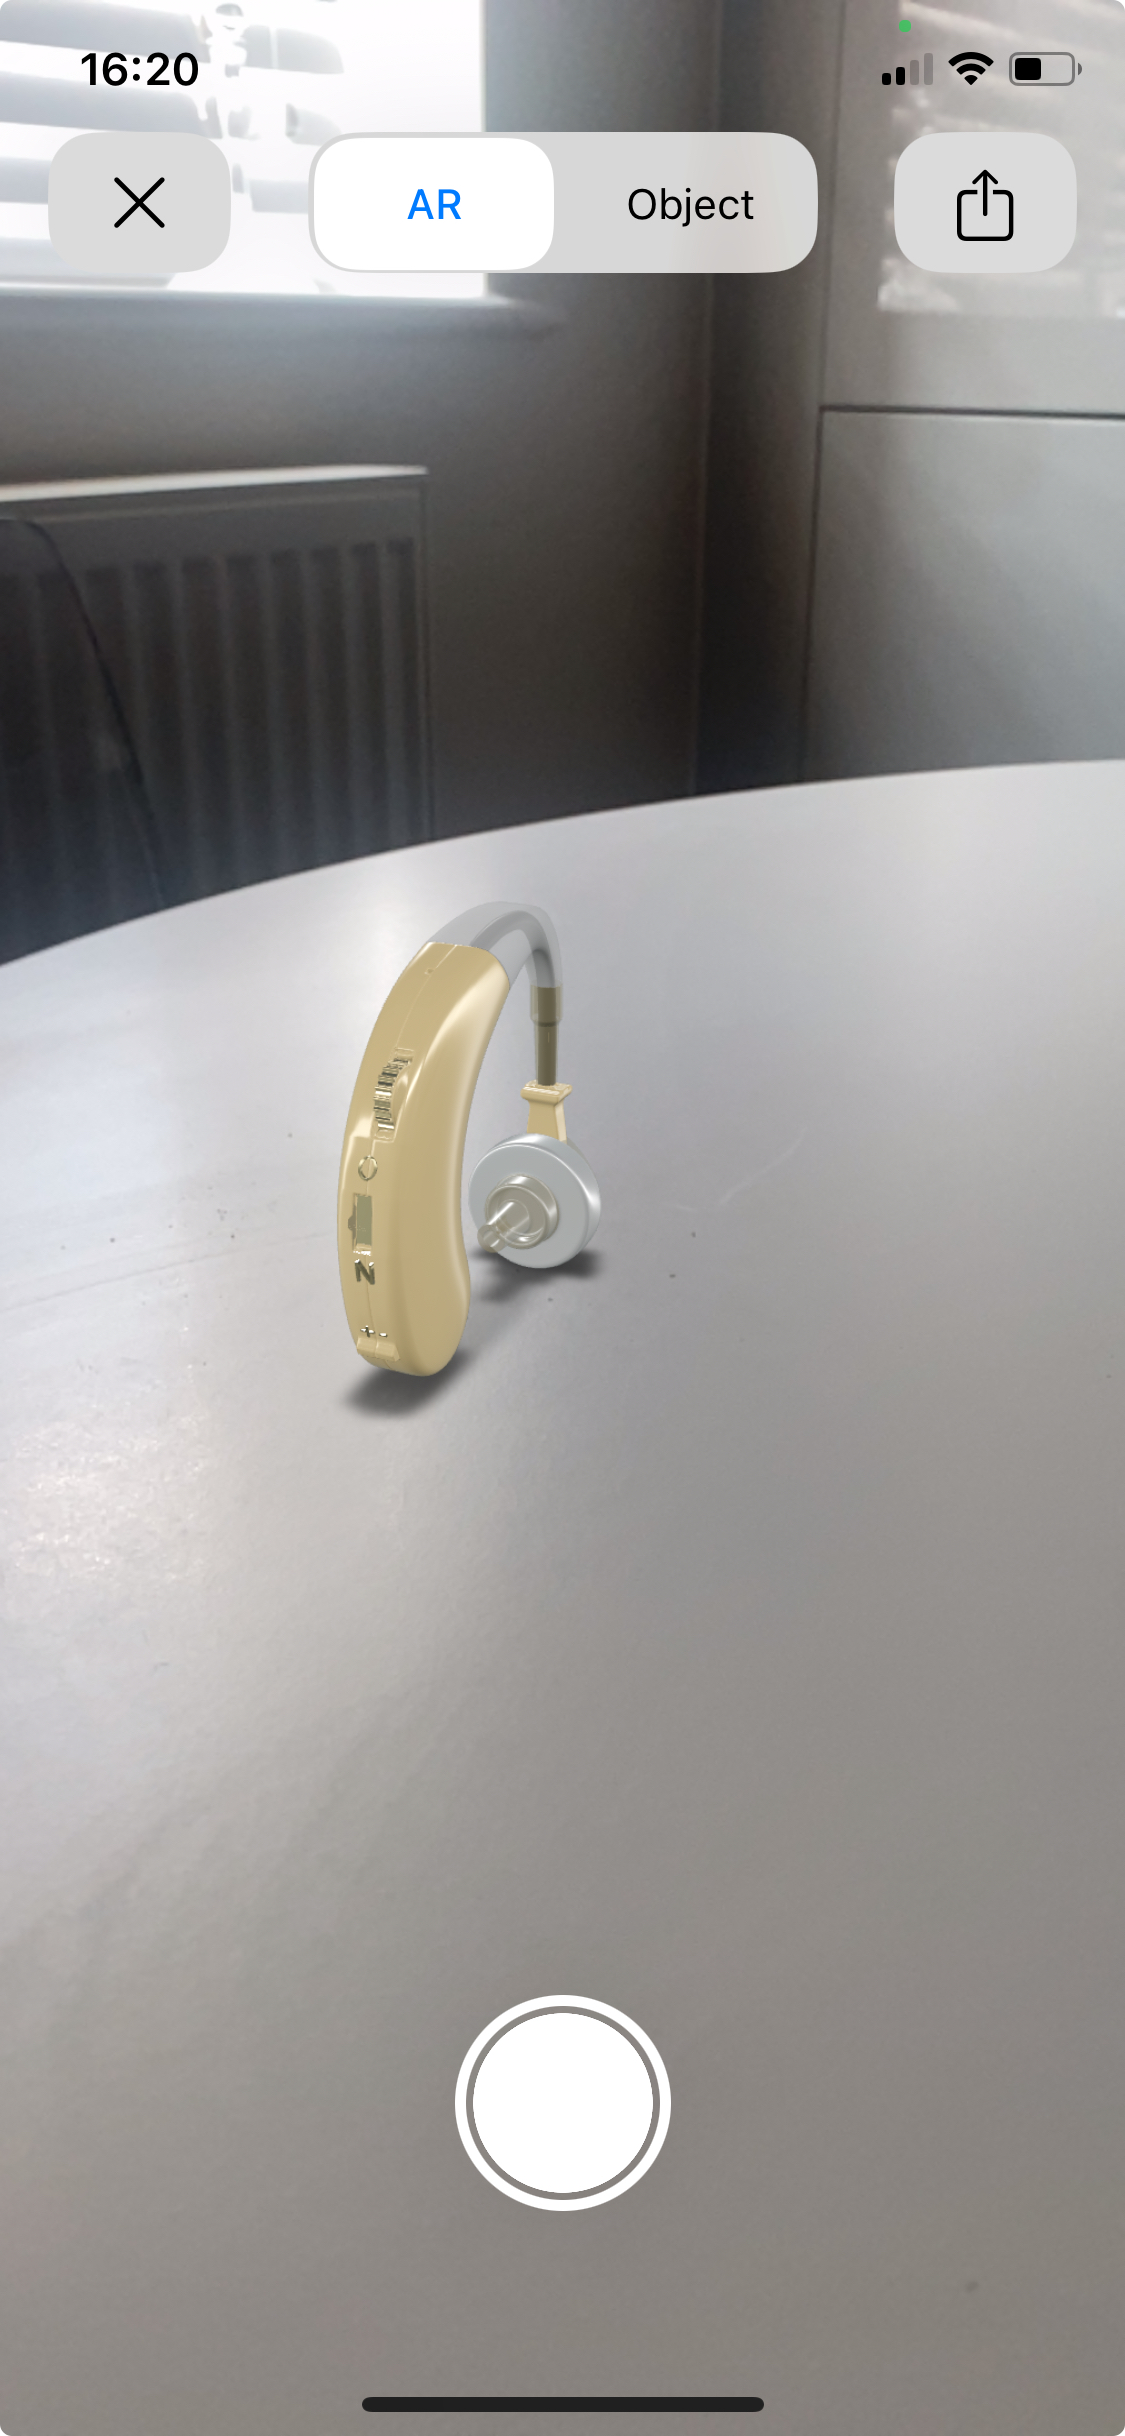
\includegraphics[height=0.5\textheight, keepaspectratio]{mobile_ar_tryon.png}
    \subcaption{Mobile AR Try-On}
\end{subfigure}
\hfill
\begin{subfigure}[b]{0.45\textwidth}
    \centering
    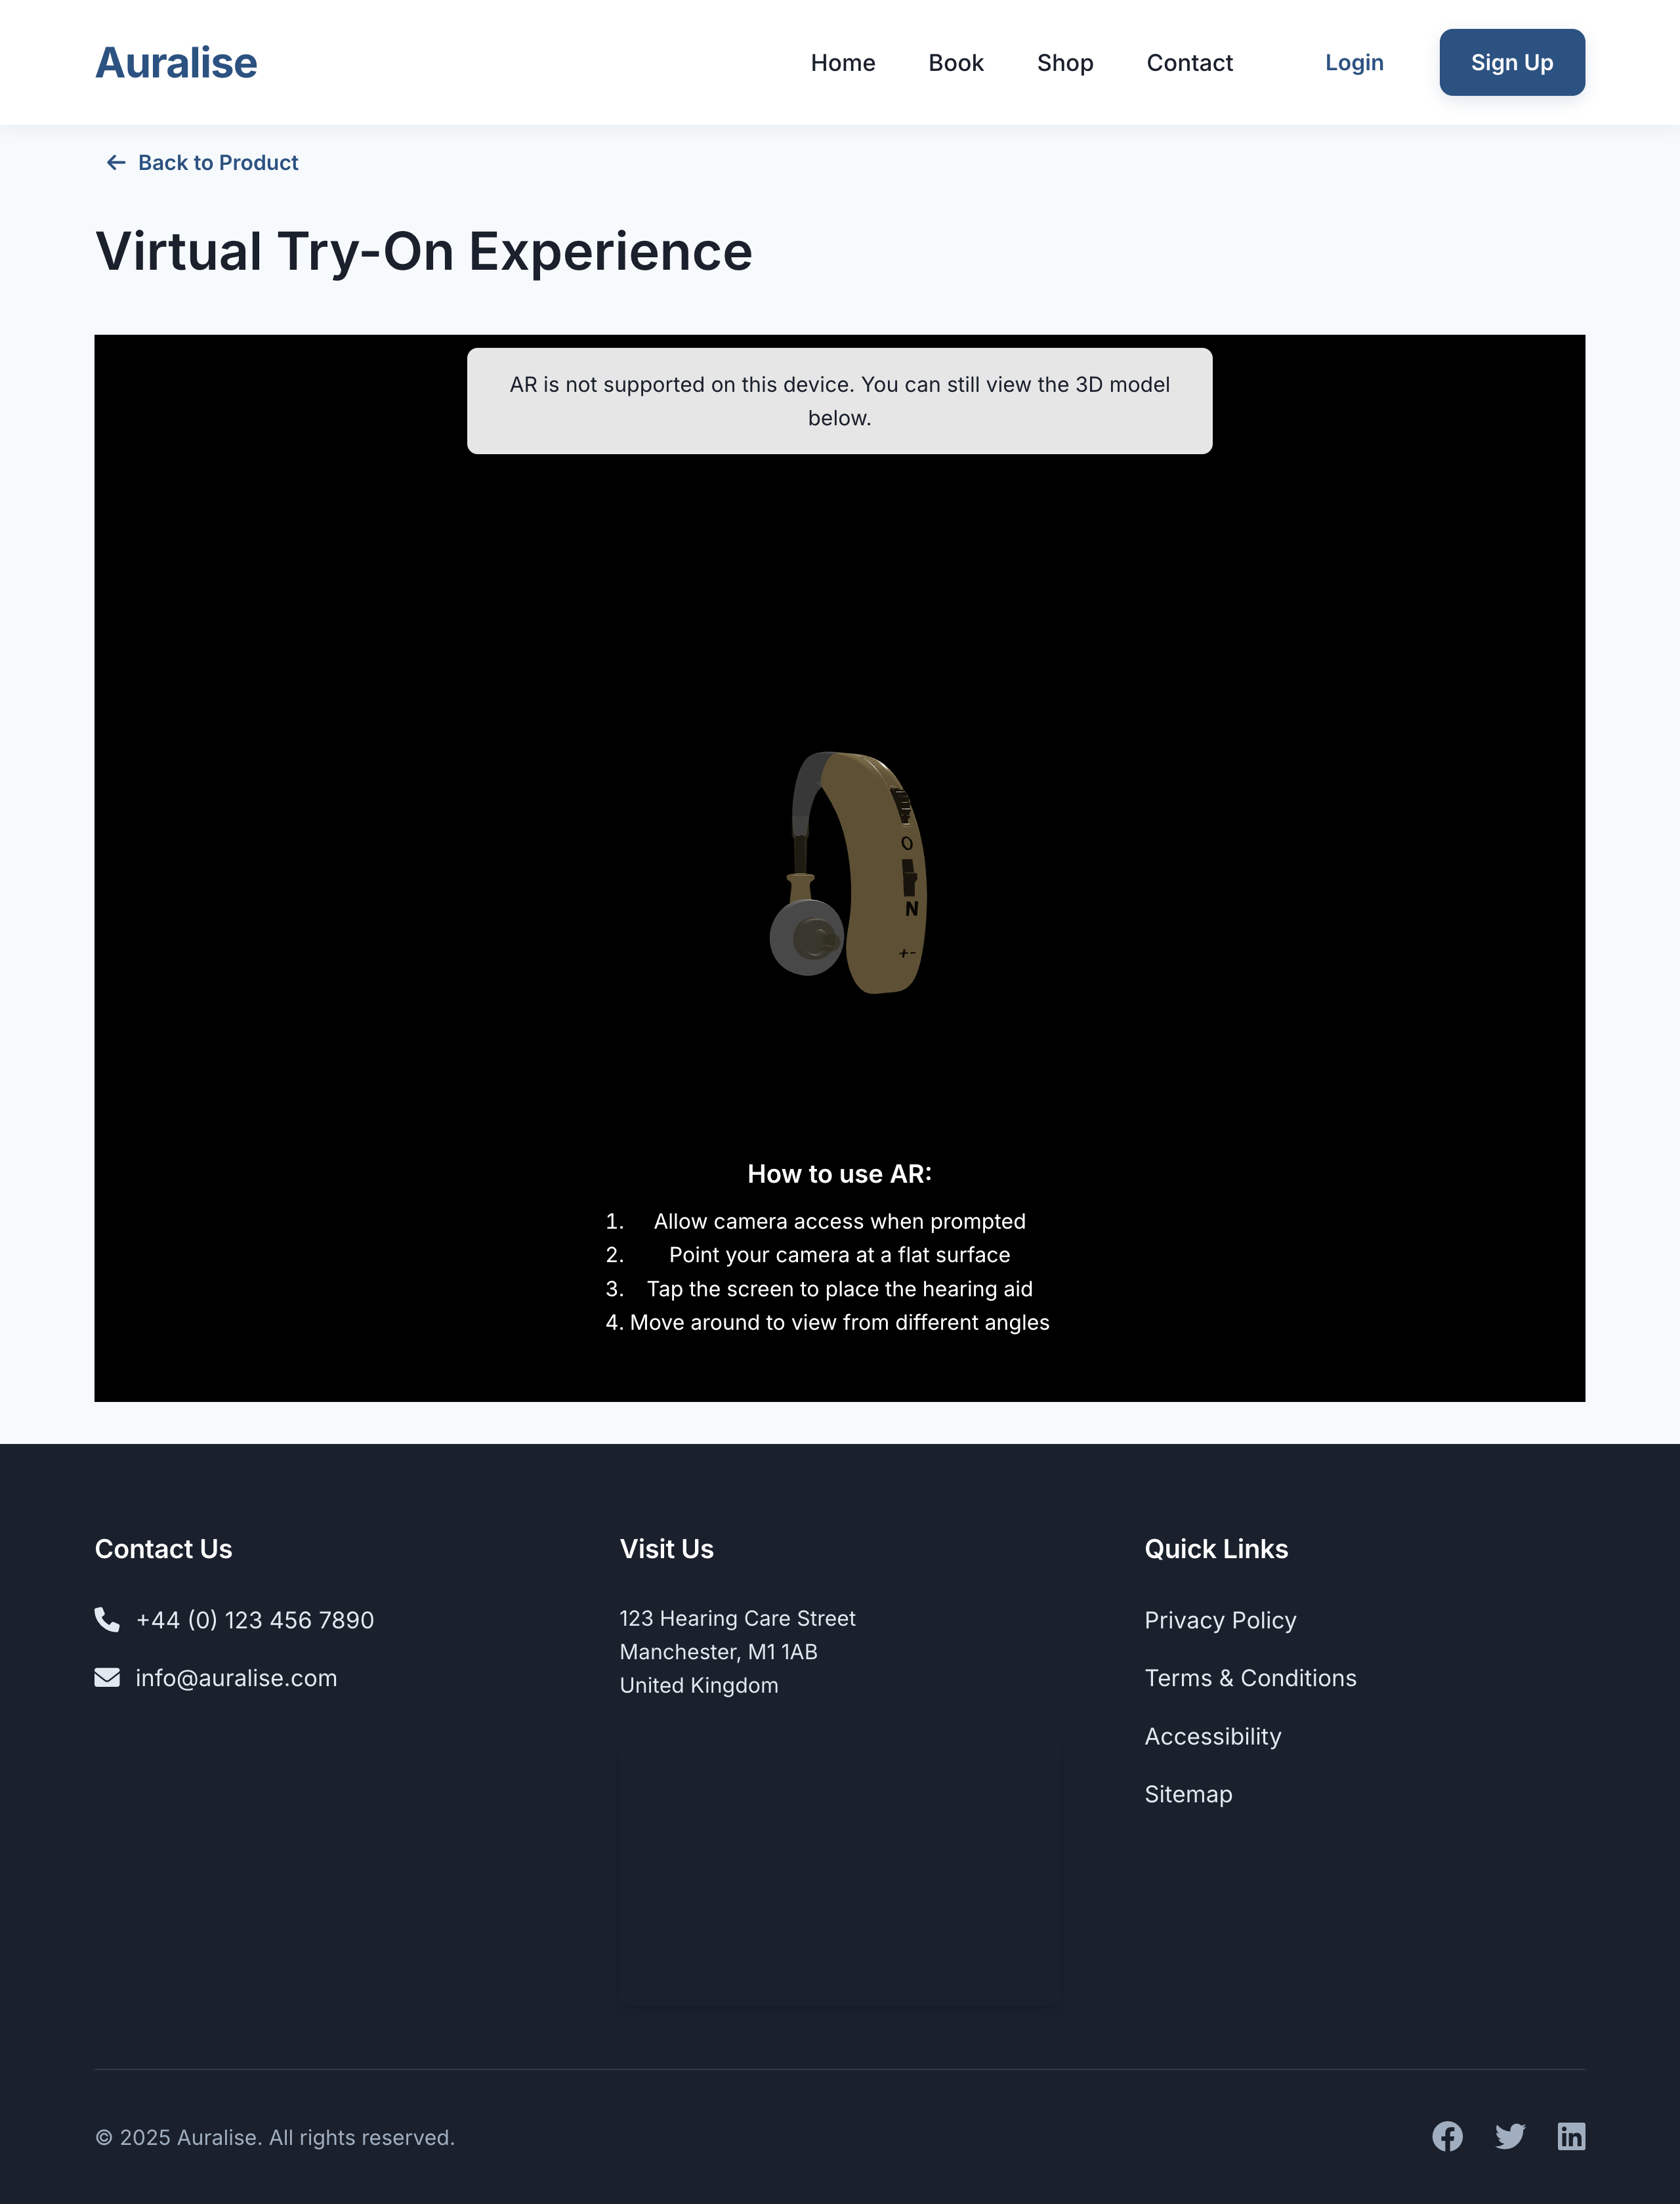
\includegraphics[height=0.4\textheight, keepaspectratio]{desktop_ar_tryon.png}
    \subcaption{Desktop AR Try-On}
\end{subfigure}
\caption{AR Try-On Experience (Mobile and Desktop)}
\label{fig:ar_tryon_experience}
\end{figure}


The Shop Page as shown in Figure~\ref{fig:shop_page} features a filterable catalog of hearing aids, allowing users to browse by type (Behind-the-Ear, In-the-Canal, etc.), brand, price range, and features. Each product card displays an image, key specifications, and price information.

The Product Detail Page as shown in Figure~\ref{fig:product_detail_page} provides comprehensive information about specific hearing aid models, including technical specifications, battery life, connectivity options, and user reviews. A 3D model viewer allows users to examine the device from all angles.

The AR Try-On feature as shown in Figure~\ref{fig:ar_tryon_experience} enables users to virtually visualise their hearing aids in their own environment:
\begin{itemize}
    \item On mobile devices, users can use their camera in real-time to see how a hearing aid would look like in their environment, and get a more accurate representation of the size and look of the hearing aids
    \item On devices that do not support AR, they can view a 3d model of the hearing aid
    \item The system uses WebXR \cite{immersive_web_2024} for Android devices and Quick Look \cite{apple_ar_quicklook_2024} for iOS devices to visualise the 3d model of the hearing aid in their own environment using AR .
\end{itemize}

This innovative AR experience helps users visualize the appearance of hearing aids before making a purchase decision, reducing anxiety about the aesthetic impact of wearing hearing aids.

\subsubsection{Appointment Booking}

\begin{figure}[H]
\centering
\begin{subfigure}[b]{0.45\textwidth}
    \centering
    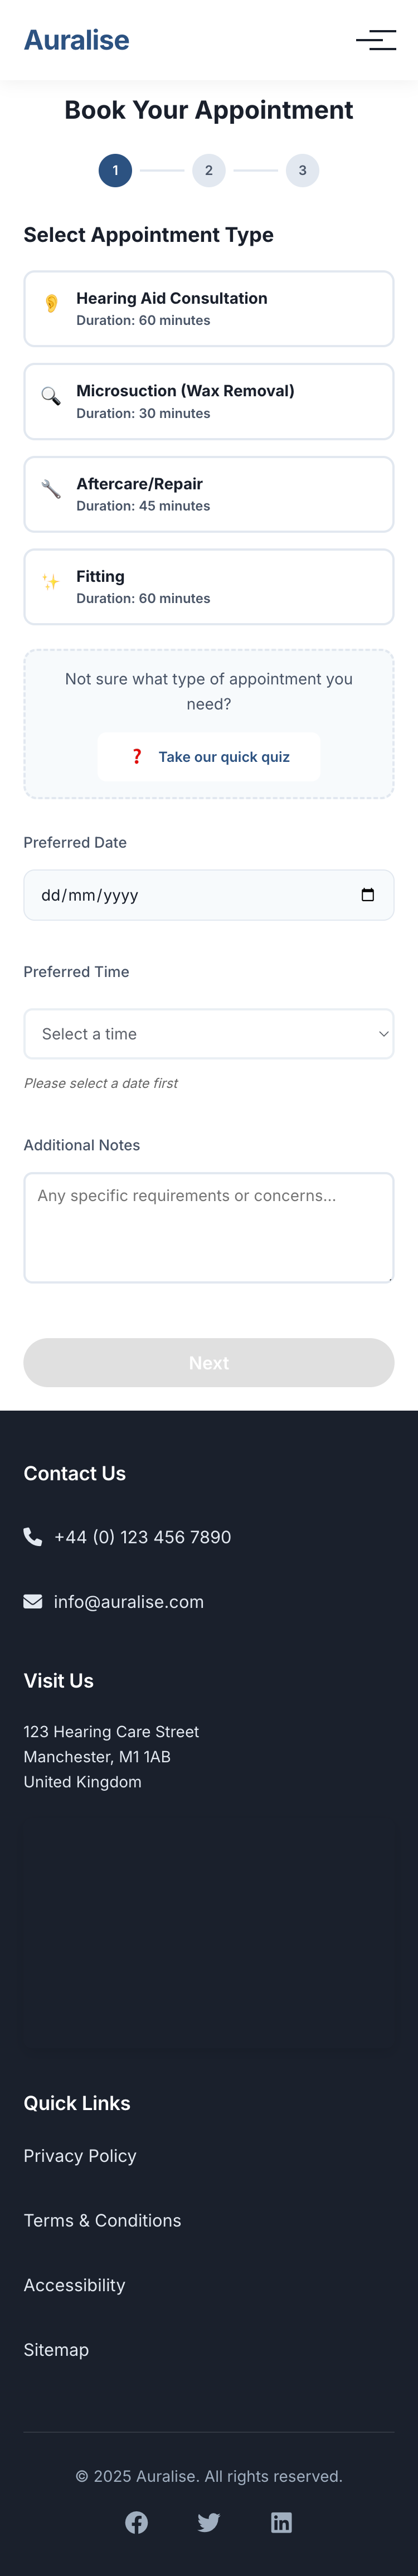
\includegraphics[height=0.5\textheight, keepaspectratio]{mobile_booking_selection.png}
    \subcaption{Mobile Booking Selection}
\end{subfigure}
\hfill
\begin{subfigure}[b]{0.45\textwidth}
    \centering
    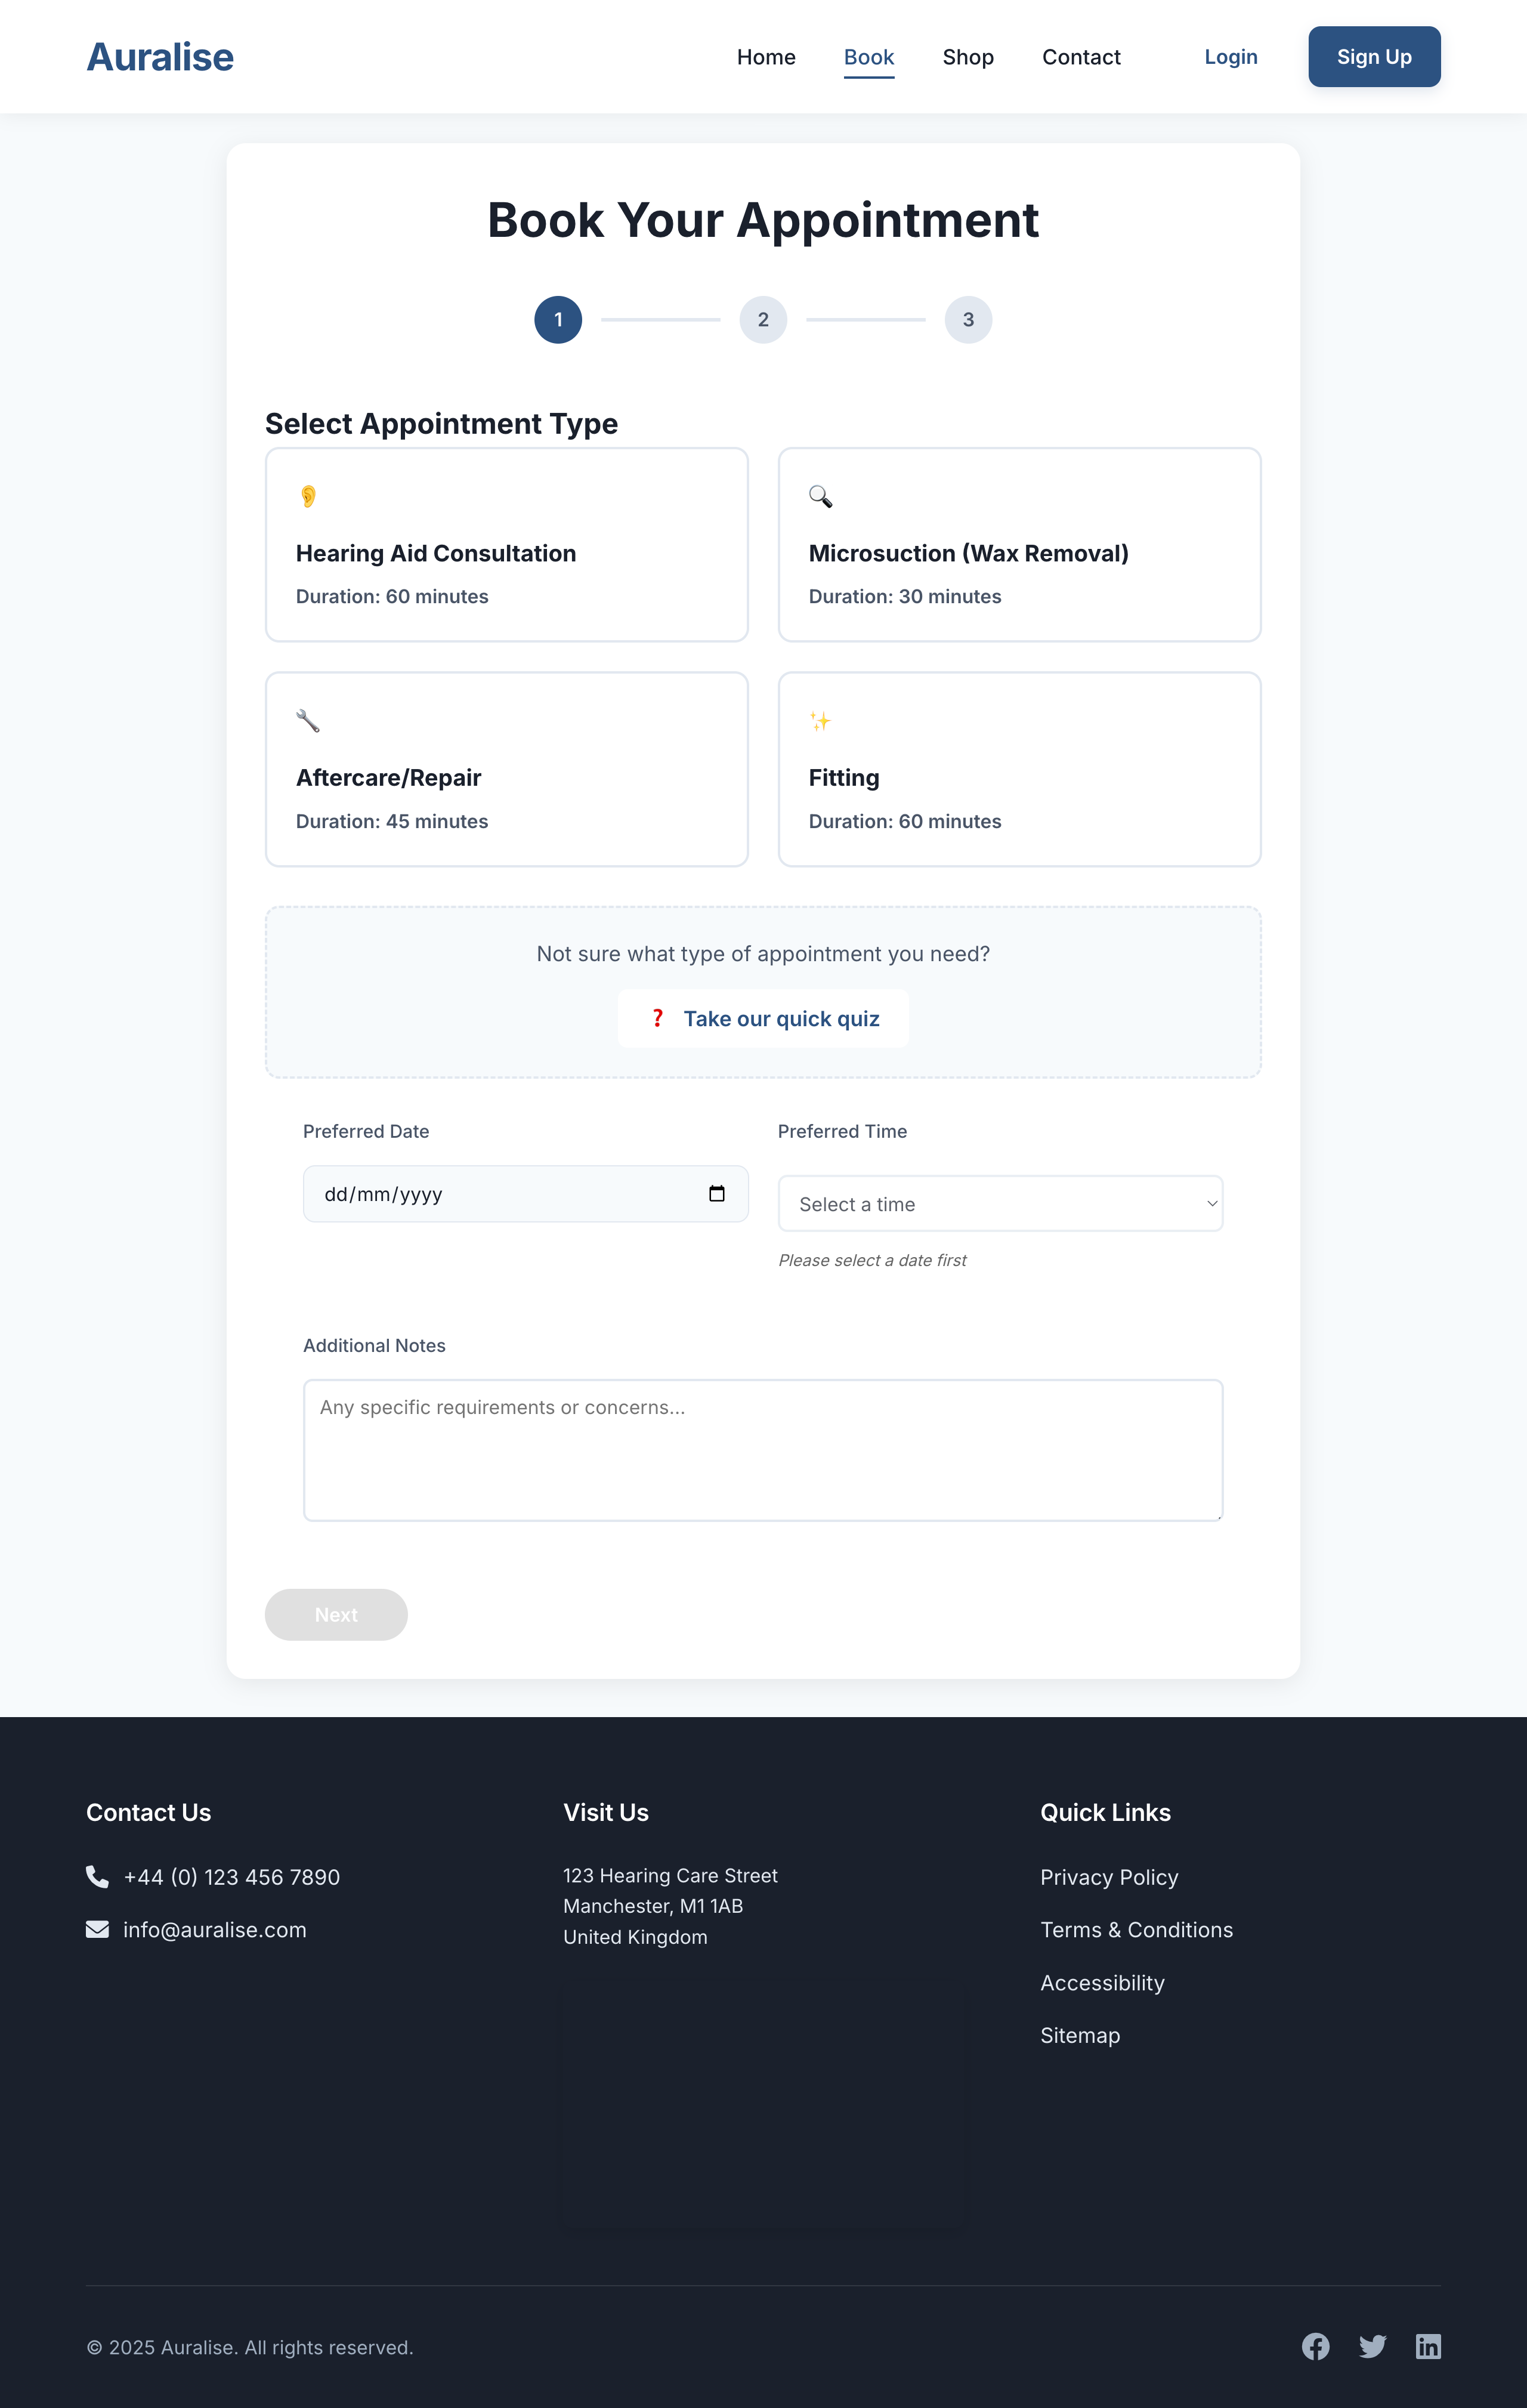
\includegraphics[height=0.5\textheight, keepaspectratio]{desktop_booking_selection.png}
    \subcaption{Desktop Booking Selection}
\end{subfigure}
\caption{Booking Selection Screen (Mobile and Desktop)}
\label{fig:booking_selection_screen}
\end{figure}

\begin{figure}[H]
\centering
\begin{subfigure}[b]{0.45\textwidth}
    \centering
    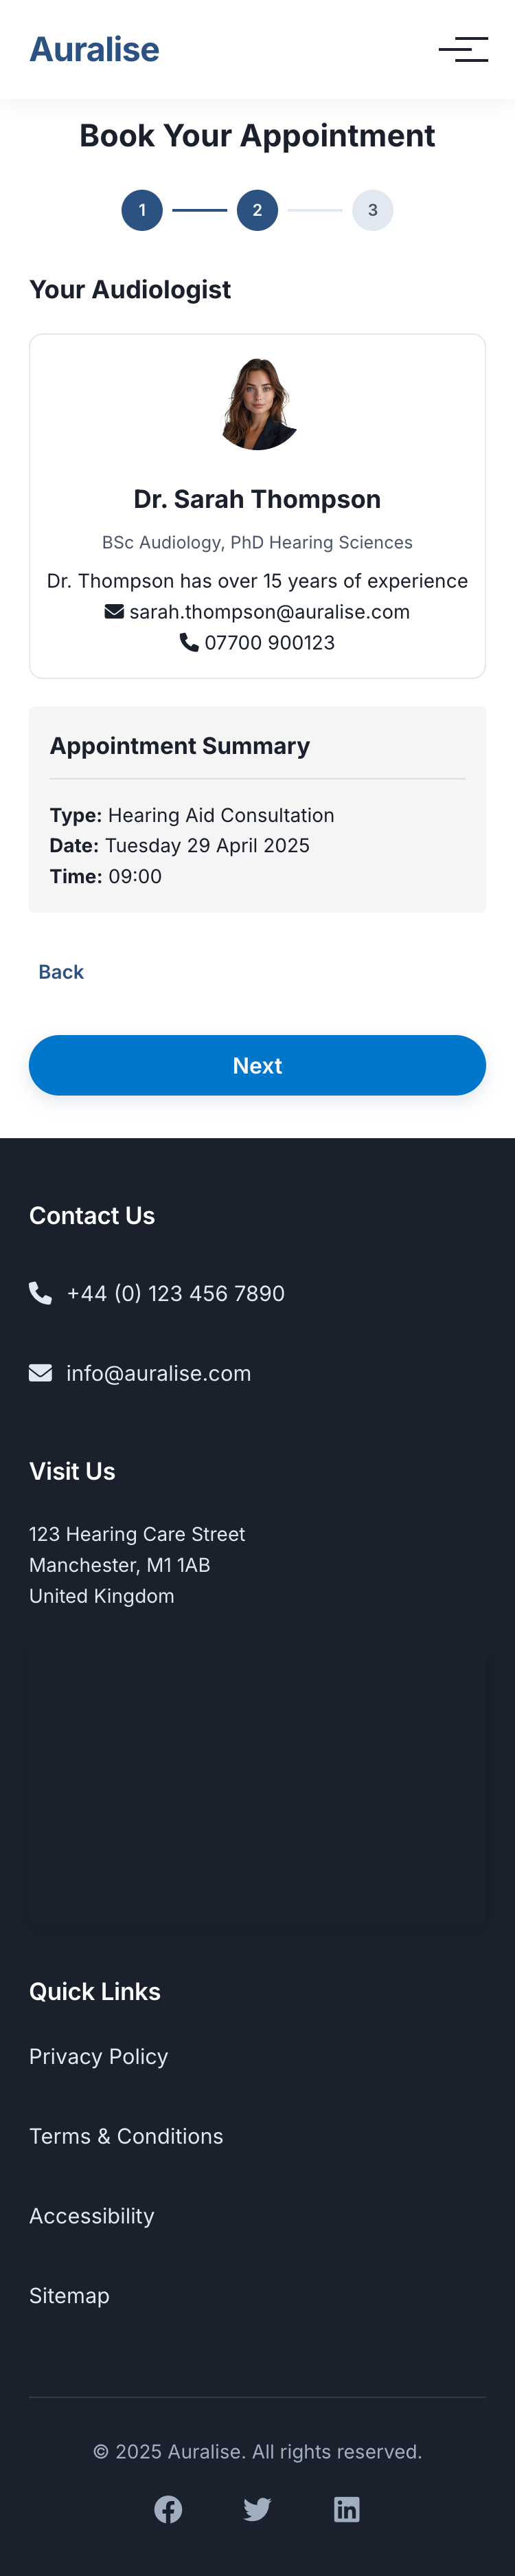
\includegraphics[height=0.5\textheight, keepaspectratio]{audiologist_picker_mobile.png}
    \subcaption{Mobile Audiologist Selection}
\end{subfigure}
\hfill
\begin{subfigure}[b]{0.45\textwidth}
    \centering
    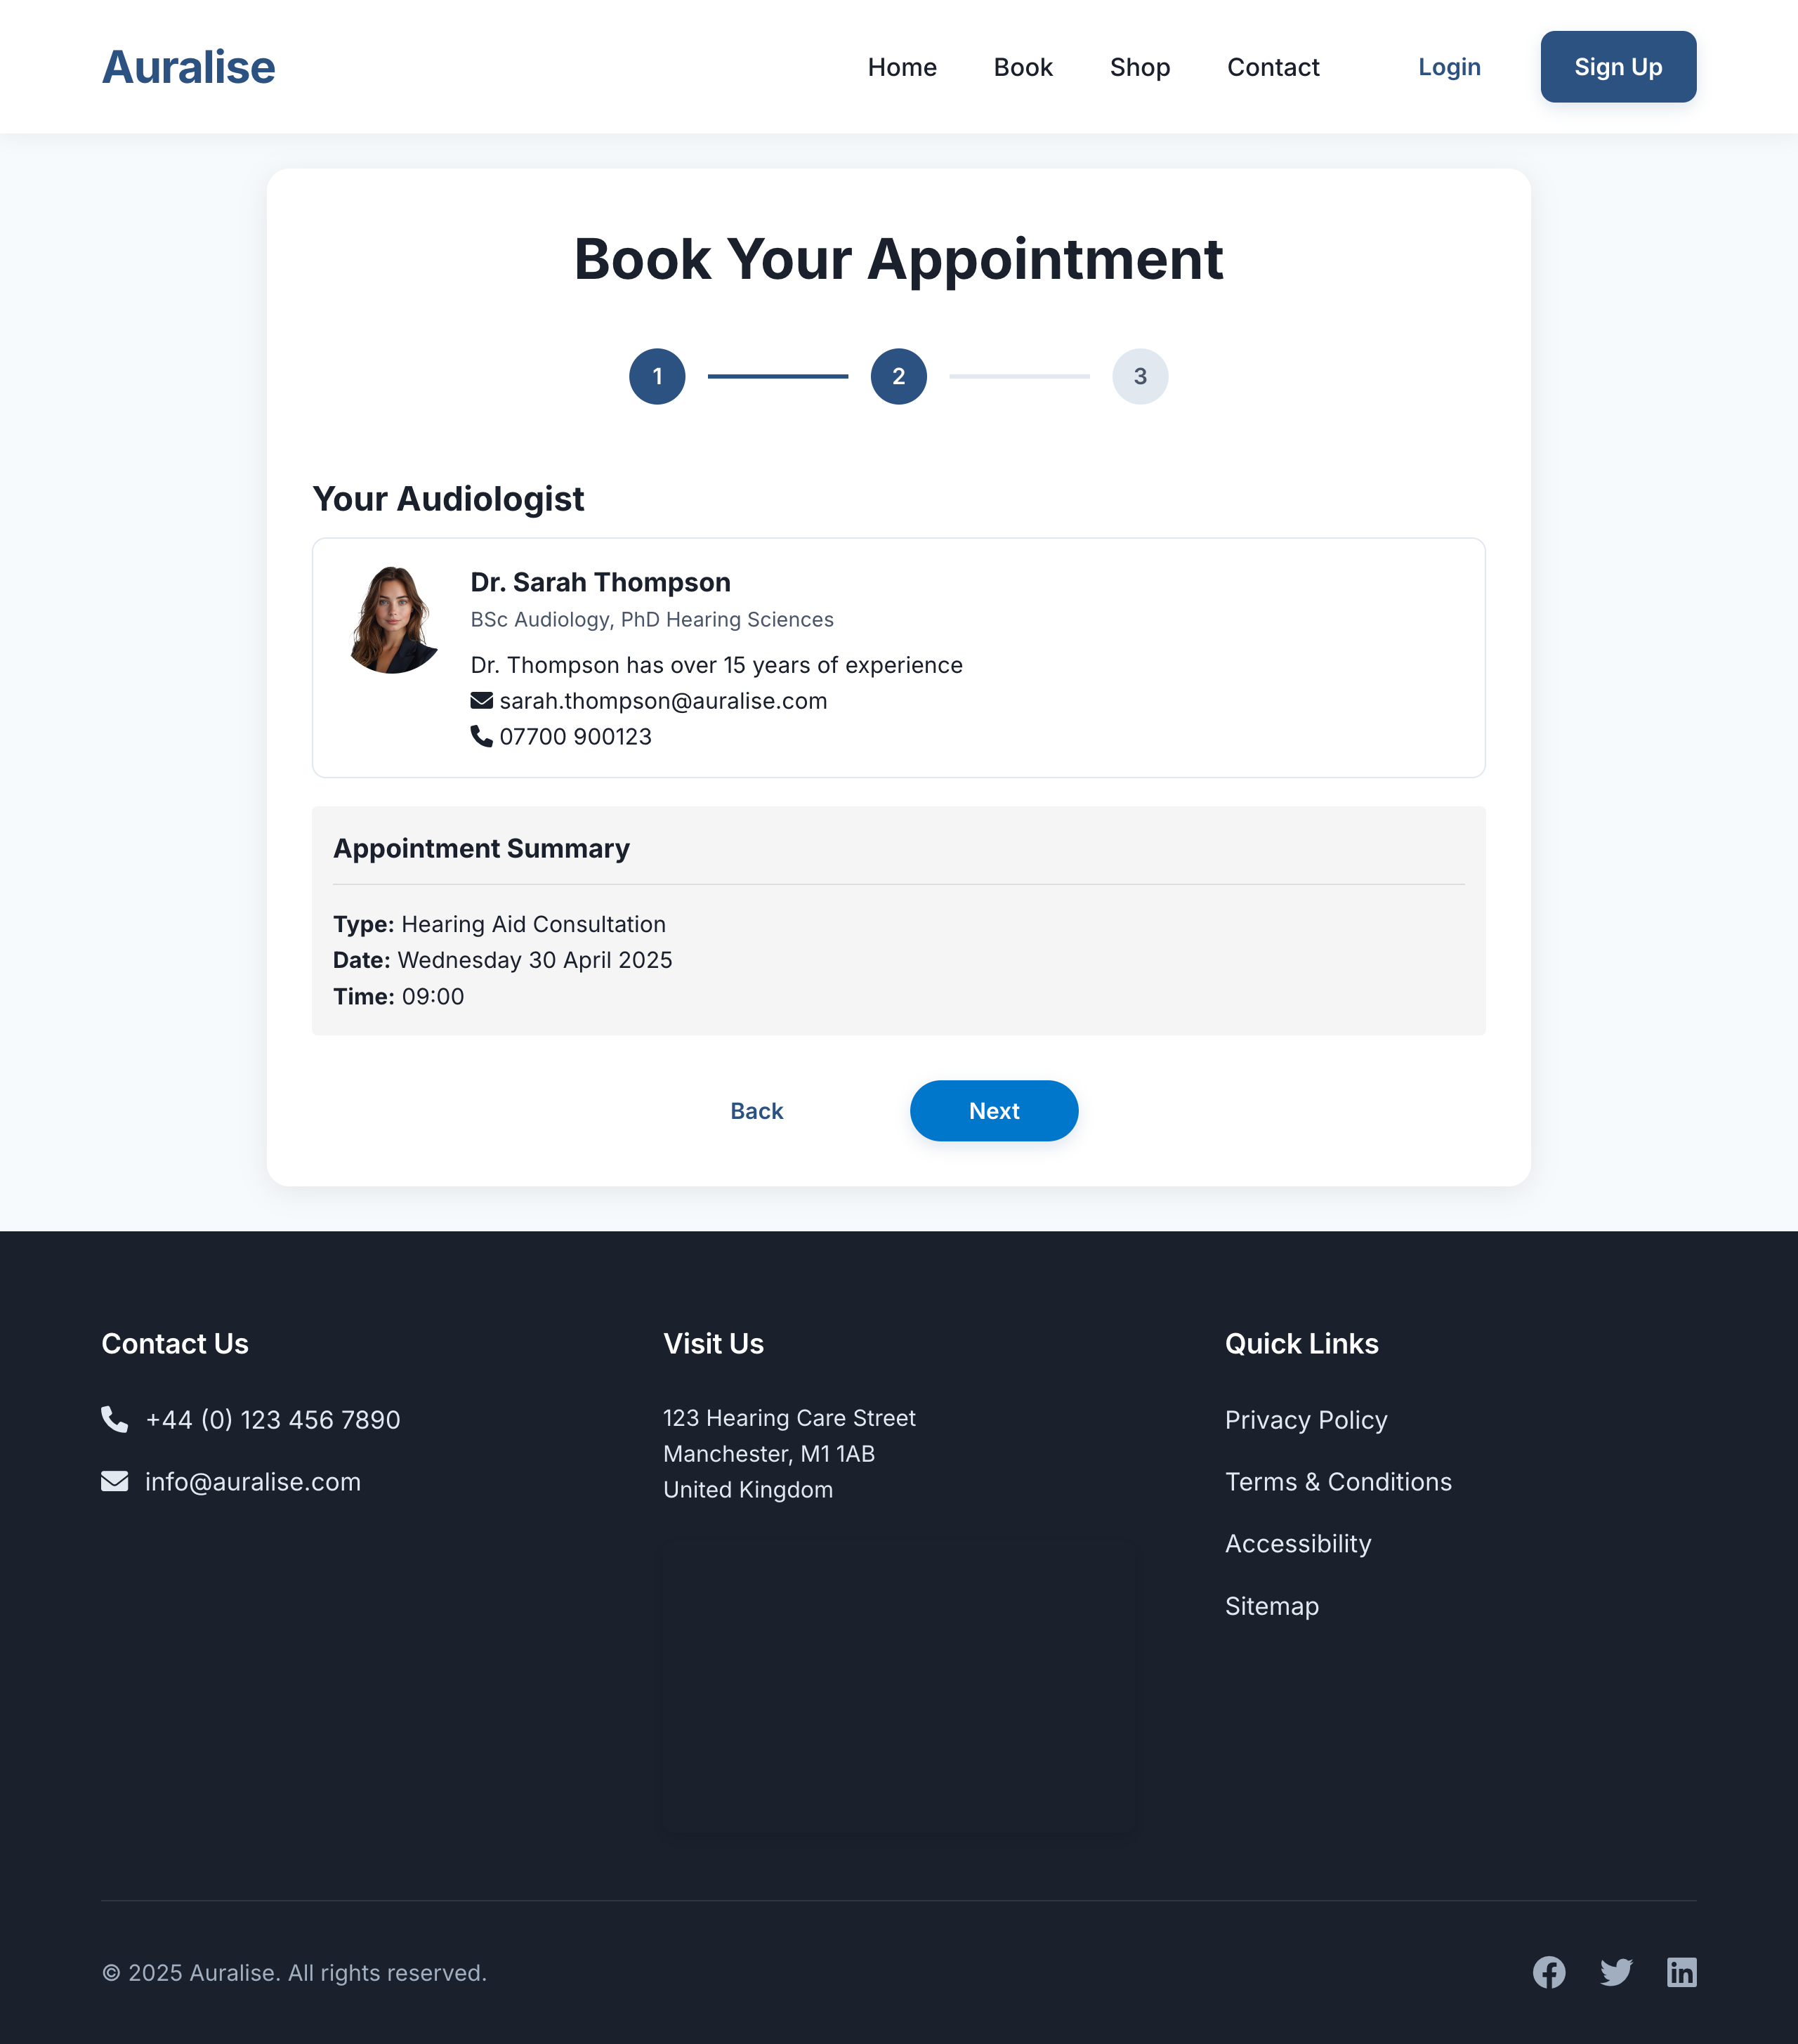
\includegraphics[height=0.3\textheight, keepaspectratio]{audiologist_picker_desktop.png}
    \subcaption{Desktop Audiologist Selection}
\end{subfigure}
\caption{Audiologist Selection Screen (Mobile and Desktop)}
\label{fig:audiologist_selection_screen}
\end{figure}

\begin{figure}[H]
\centering
\begin{subfigure}[b]{0.45\textwidth}
    \centering
    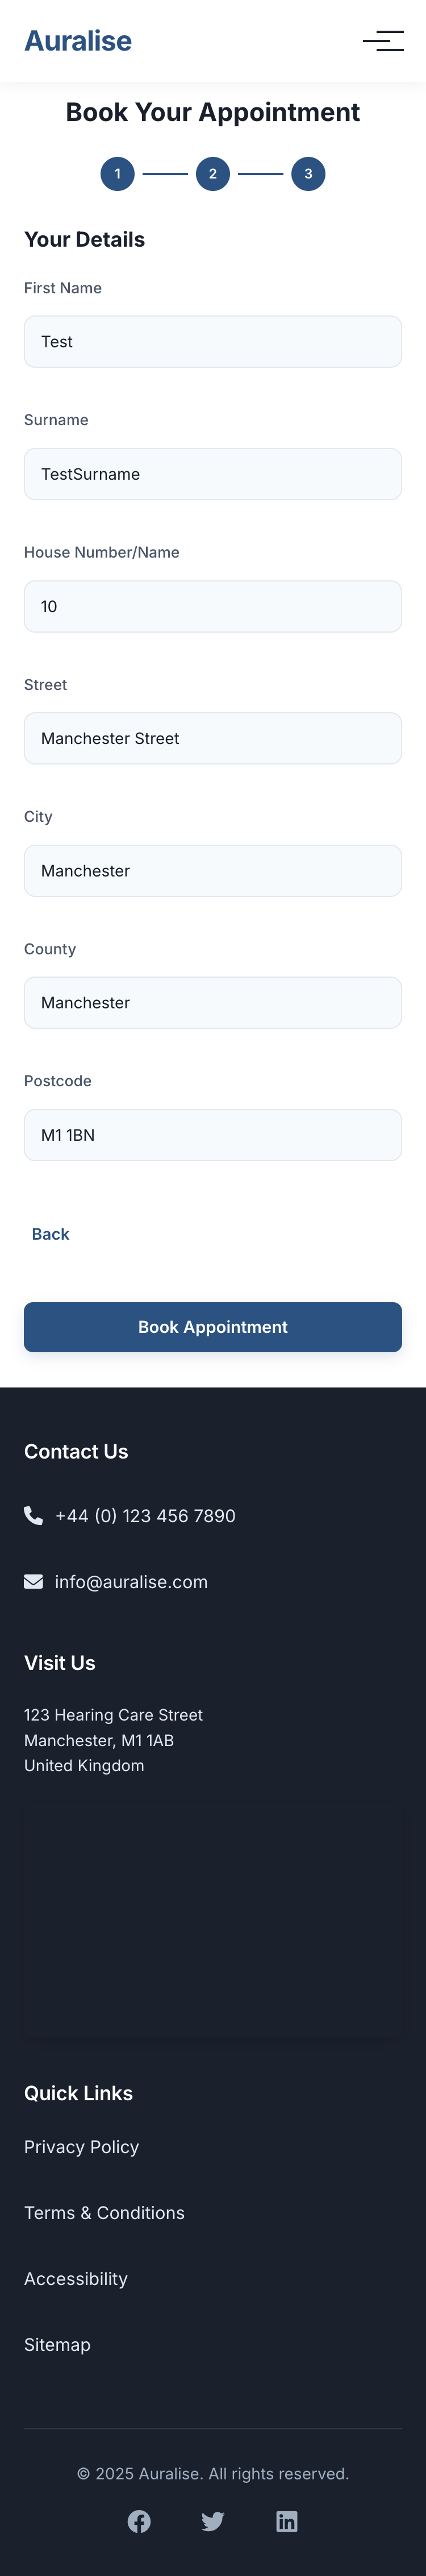
\includegraphics[height=0.5\textheight, keepaspectratio]{details_mobile.png}
    \subcaption{Mobile Details Entry}
\end{subfigure}
\hfill
\begin{subfigure}[b]{0.45\textwidth}
    \centering
    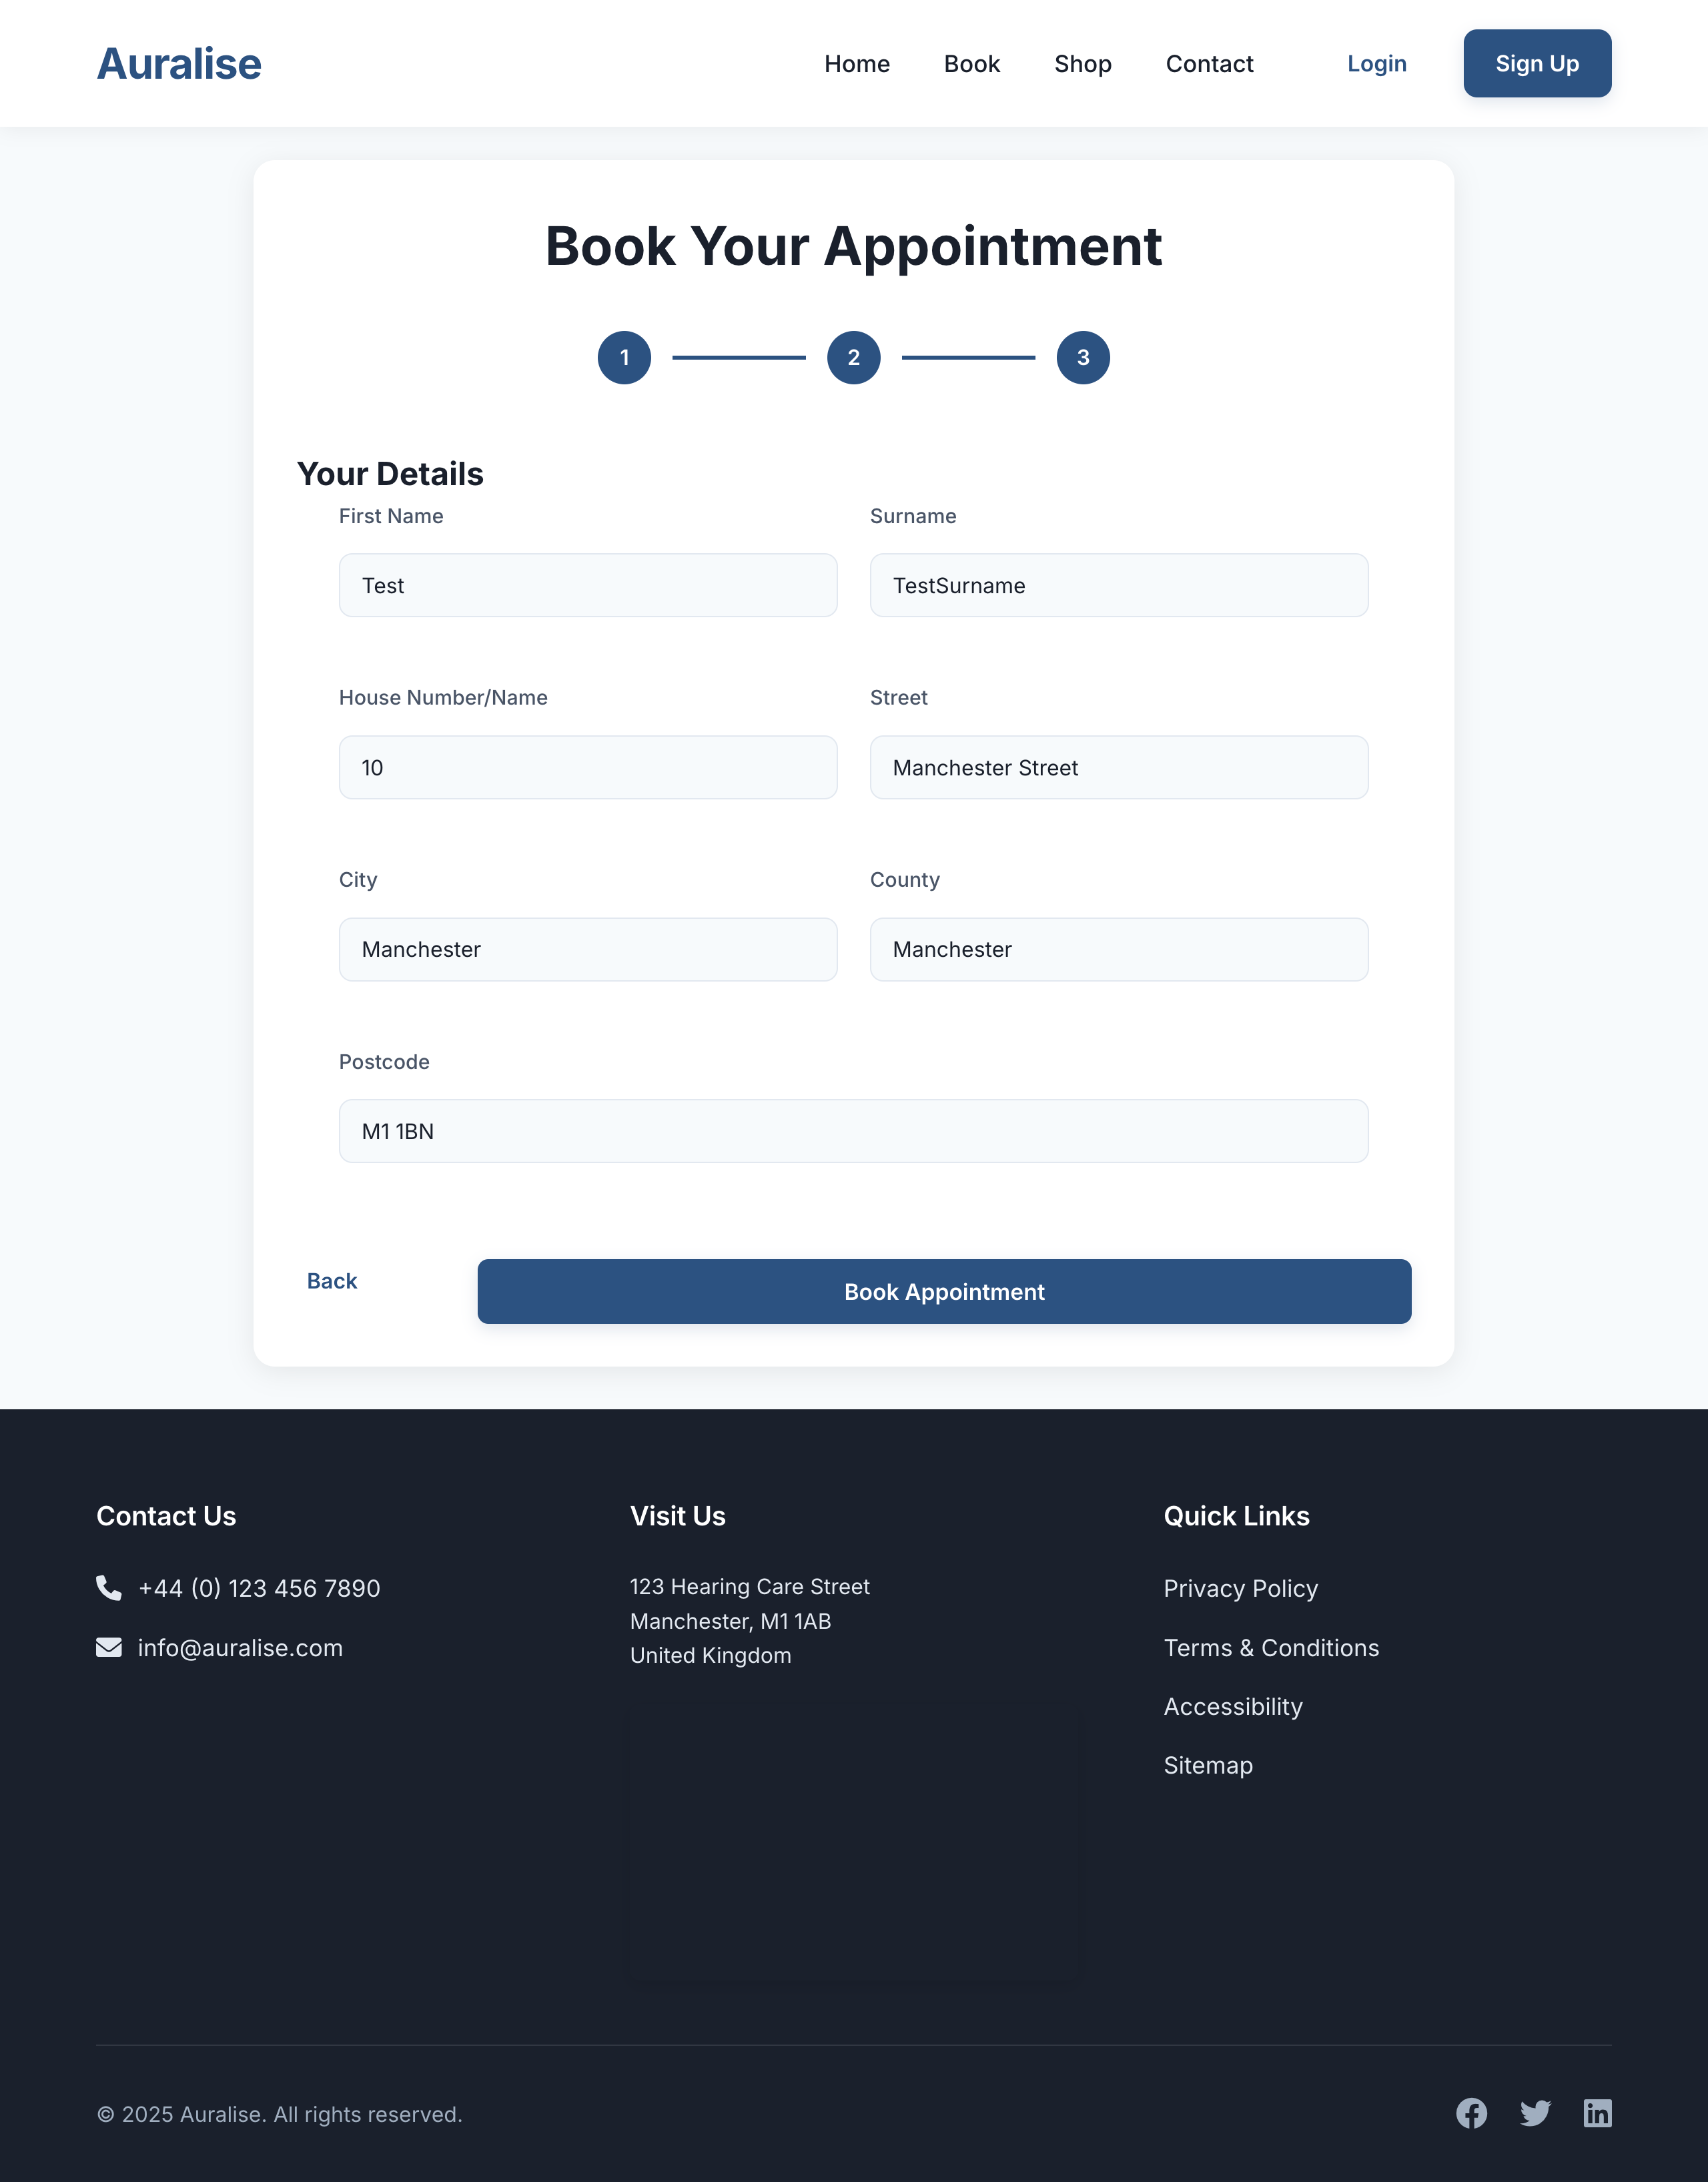
\includegraphics[height=0.3\textheight, keepaspectratio]{details_desktop.png}
    \subcaption{Desktop Details Entry}
\end{subfigure}
\caption{Details Entry Screen (Mobile and Desktop)}
\label{fig:details_entry_screen}
\end{figure}

\begin{figure}[H]
\centering
\begin{subfigure}[b]{0.45\textwidth}
    \centering
    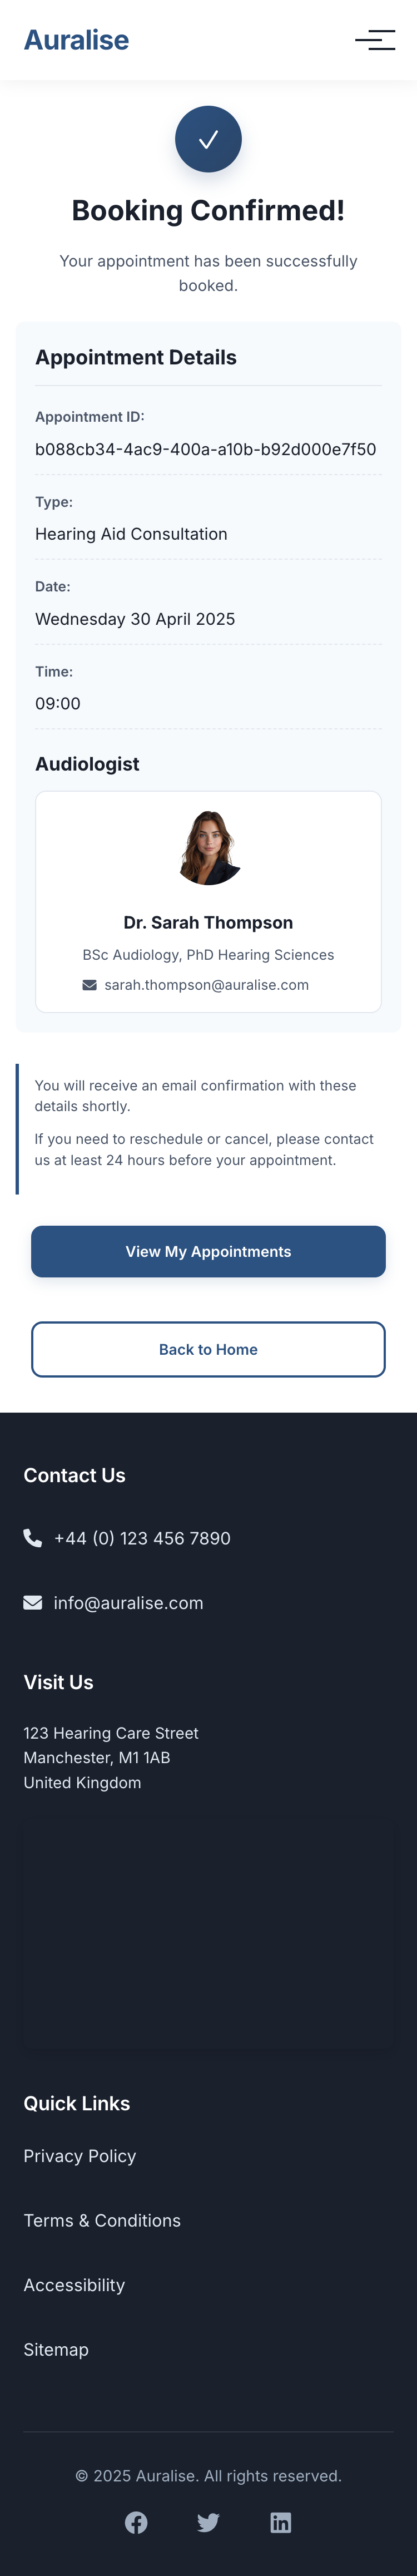
\includegraphics[height=0.5\textheight, keepaspectratio]{booking_confirmation_mobile.png}
    \subcaption{Mobile Booking Confirmation}
\end{subfigure}
\hfill
\begin{subfigure}[b]{0.45\textwidth}
    \centering
    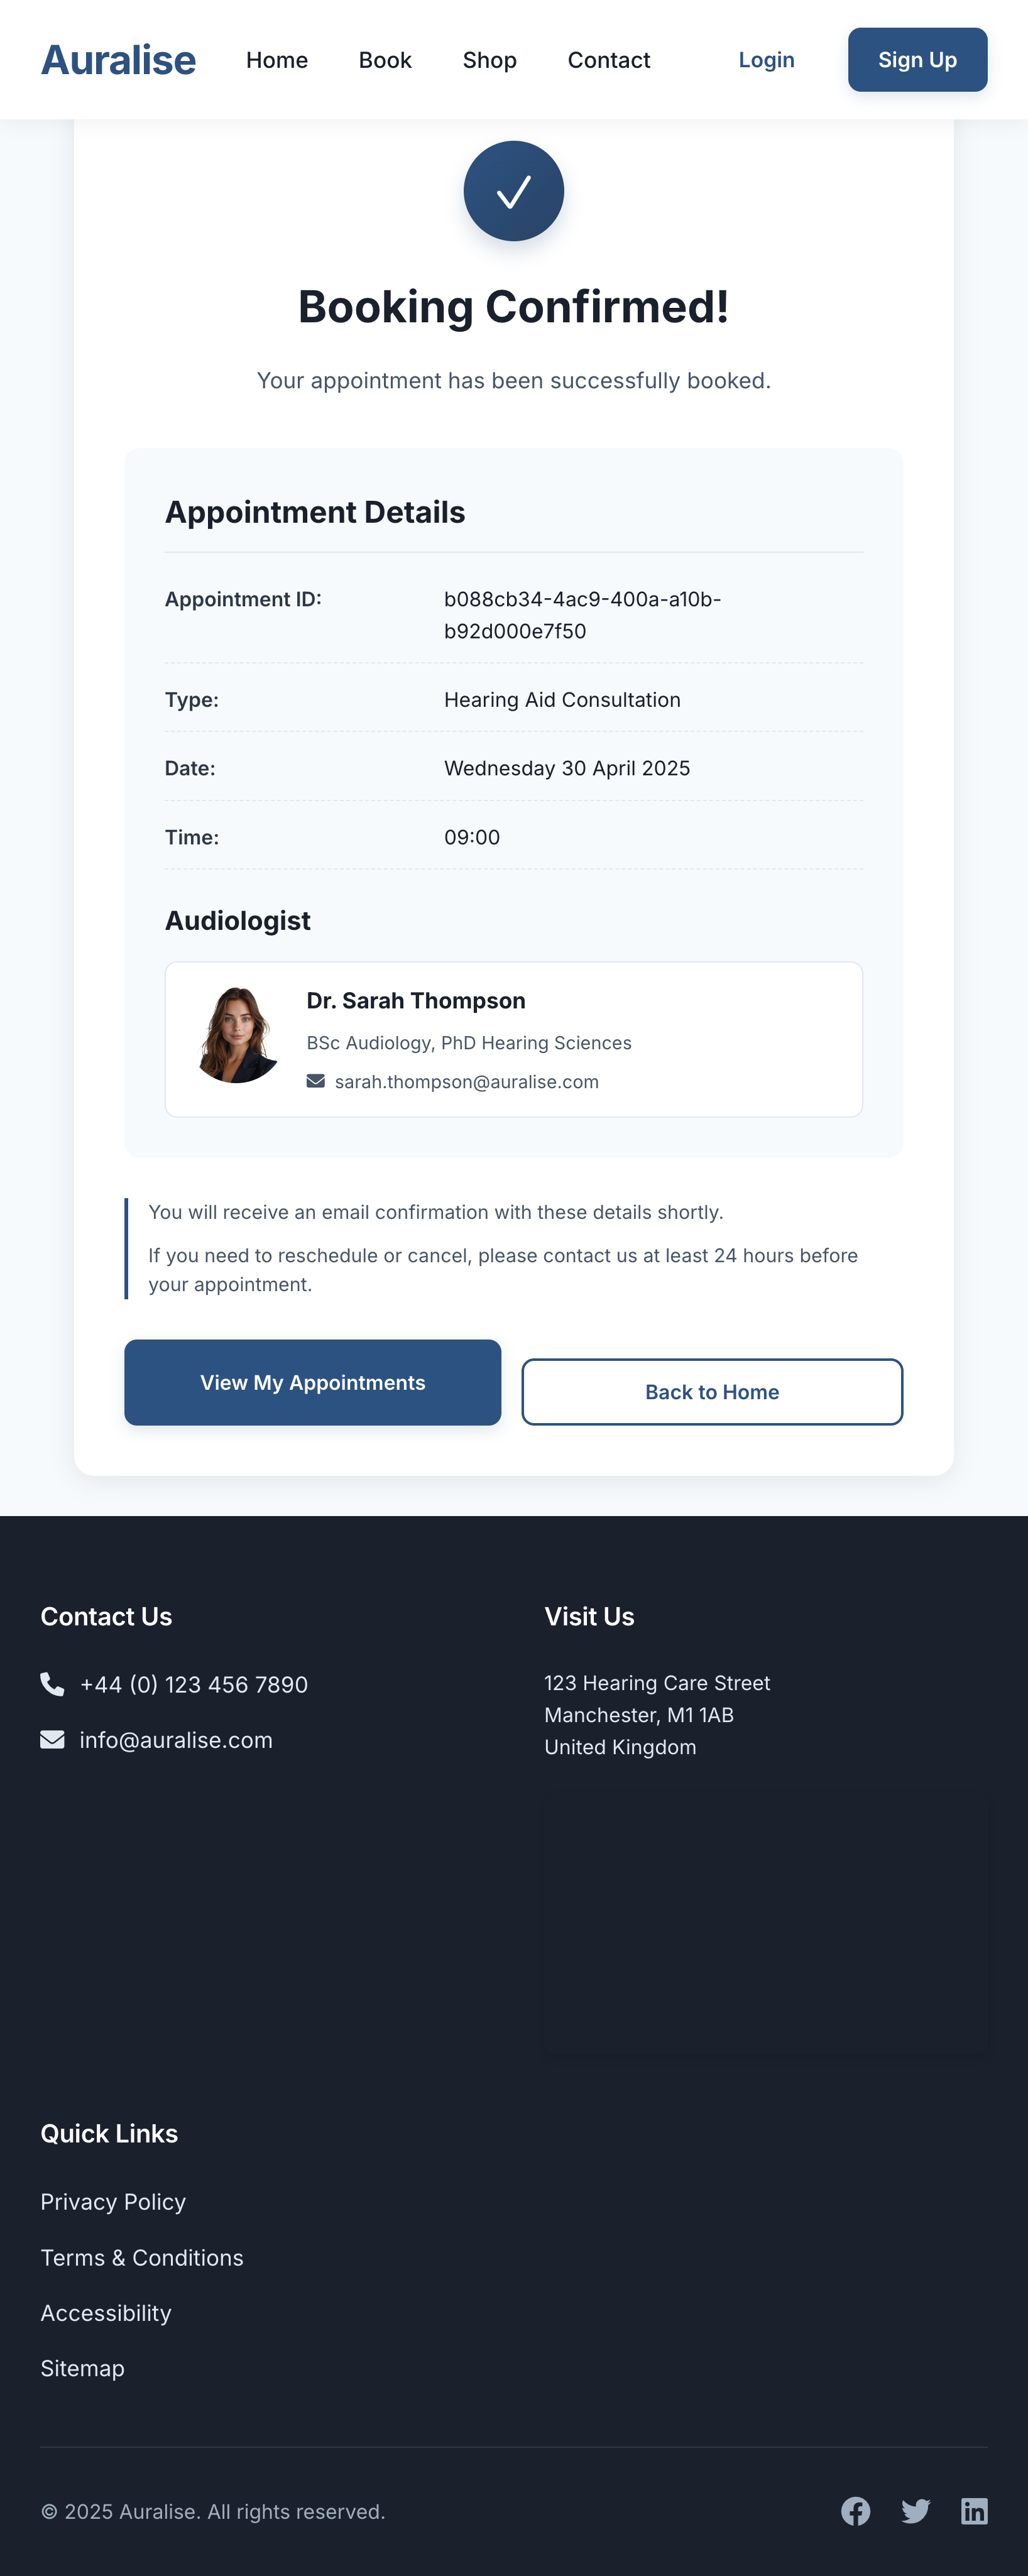
\includegraphics[height=0.5\textheight, keepaspectratio]{booking_confirmation_desktop.png}
    \subcaption{Desktop Booking Confirmation}
\end{subfigure}
\caption{Booking Confirmation (Mobile and Desktop)}
\label{fig:booking_confirmation}
\end{figure}


The Appointment Booking system allows users to schedule consultations with audiologists. The process begins with selecting an appointment type from four options as shown in Figure~\ref{fig:booking_selection_screen}:
\begin{enumerate}
    \item Hearing Aid Consultation (60 minutes)
    \item Microsuction/Wax Removal (30 minutes)
    \item Aftercare/Repair (45 minutes)
    \item Fitting (60 minutes)
\end{enumerate}

Users then select a preferred date and time from available slots. The system only shows time slots when audiologists are available, preventing double-bookings.

After confirming appointment details and providing contact information as shown in Figure~\ref{fig:details_entry_screen}, users receive a confirmation email with appointment details and any preparation instructions as shown in Figure~\ref{fig:booking_confirmation}. The system also sends reminders as the appointment date approaches.

\subsubsection{User Profile and Hearing Journey}

\begin{figure}[H]
\centering
\begin{subfigure}[b]{0.45\textwidth}
    \centering
    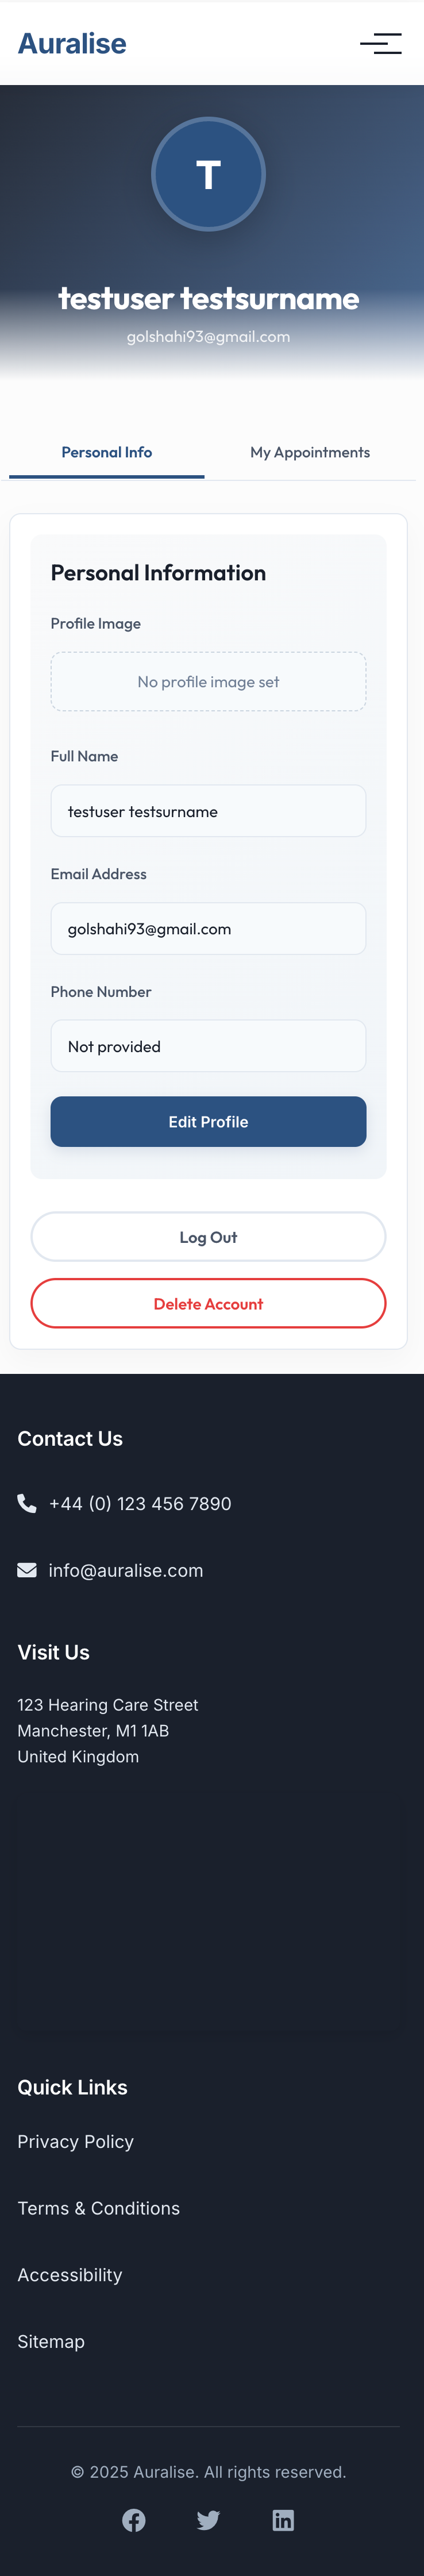
\includegraphics[height=0.5\textheight, keepaspectratio]{mobile_user_profile.png}
    \subcaption{Mobile User Profile}
\end{subfigure}
\hfill
\begin{subfigure}[b]{0.45\textwidth}
    \centering
    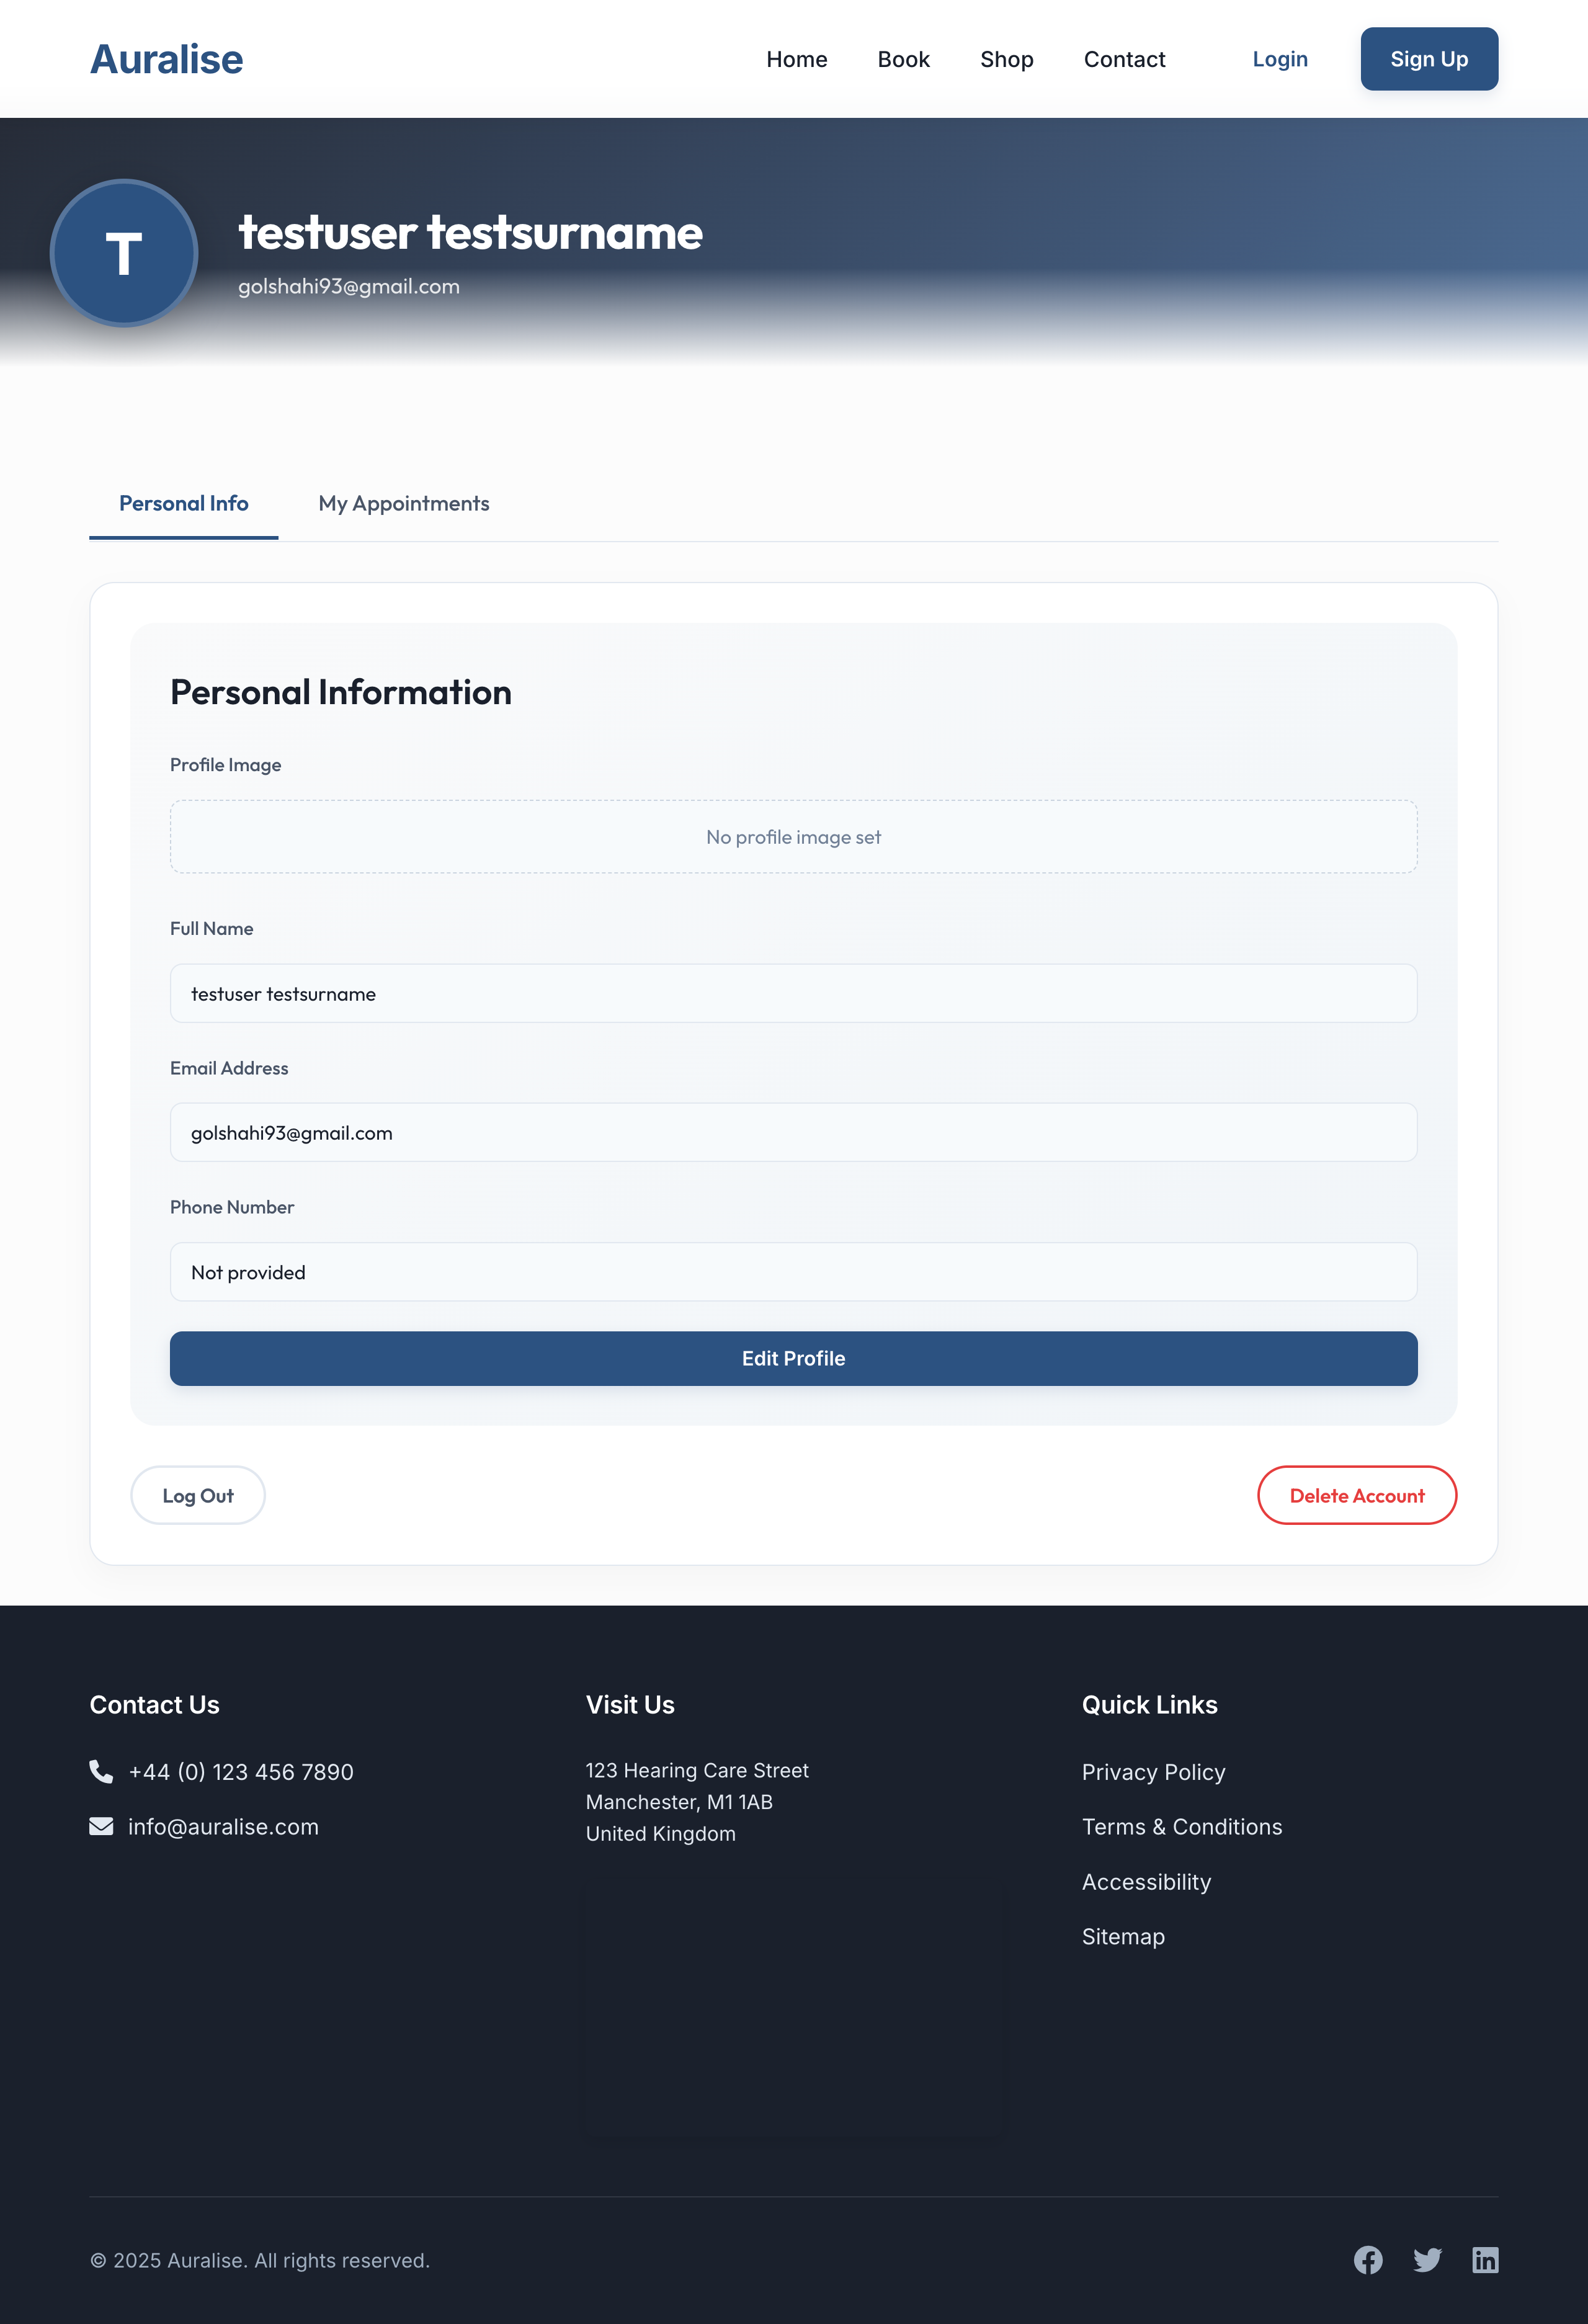
\includegraphics[height=0.4\textheight, keepaspectratio]{desktop_user_profile.png}
    \subcaption{Desktop User Profile}
\end{subfigure}
\caption{User Profile Page (Mobile and Desktop)}
\label{fig:user_profile_page}
\end{figure}

\begin{figure}[H]
\centering
\begin{subfigure}[b]{0.45\textwidth}
    \centering
    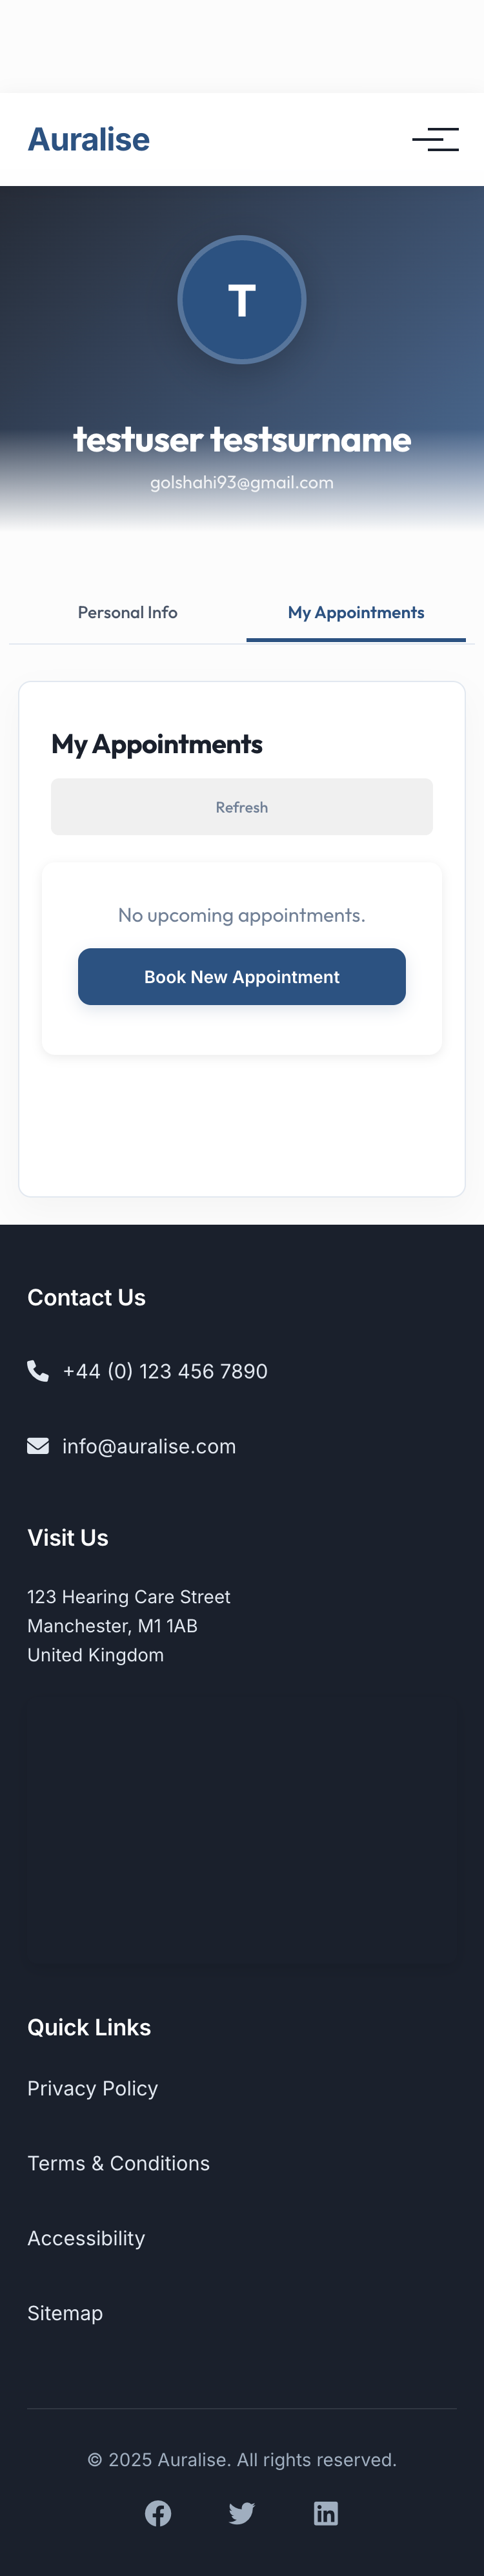
\includegraphics[height=0.5\textheight, keepaspectratio]{mobile_appointment_history.png}
    \subcaption{Mobile Appointment History}
\end{subfigure}
\hfill
\begin{subfigure}[b]{0.45\textwidth}
    \centering
    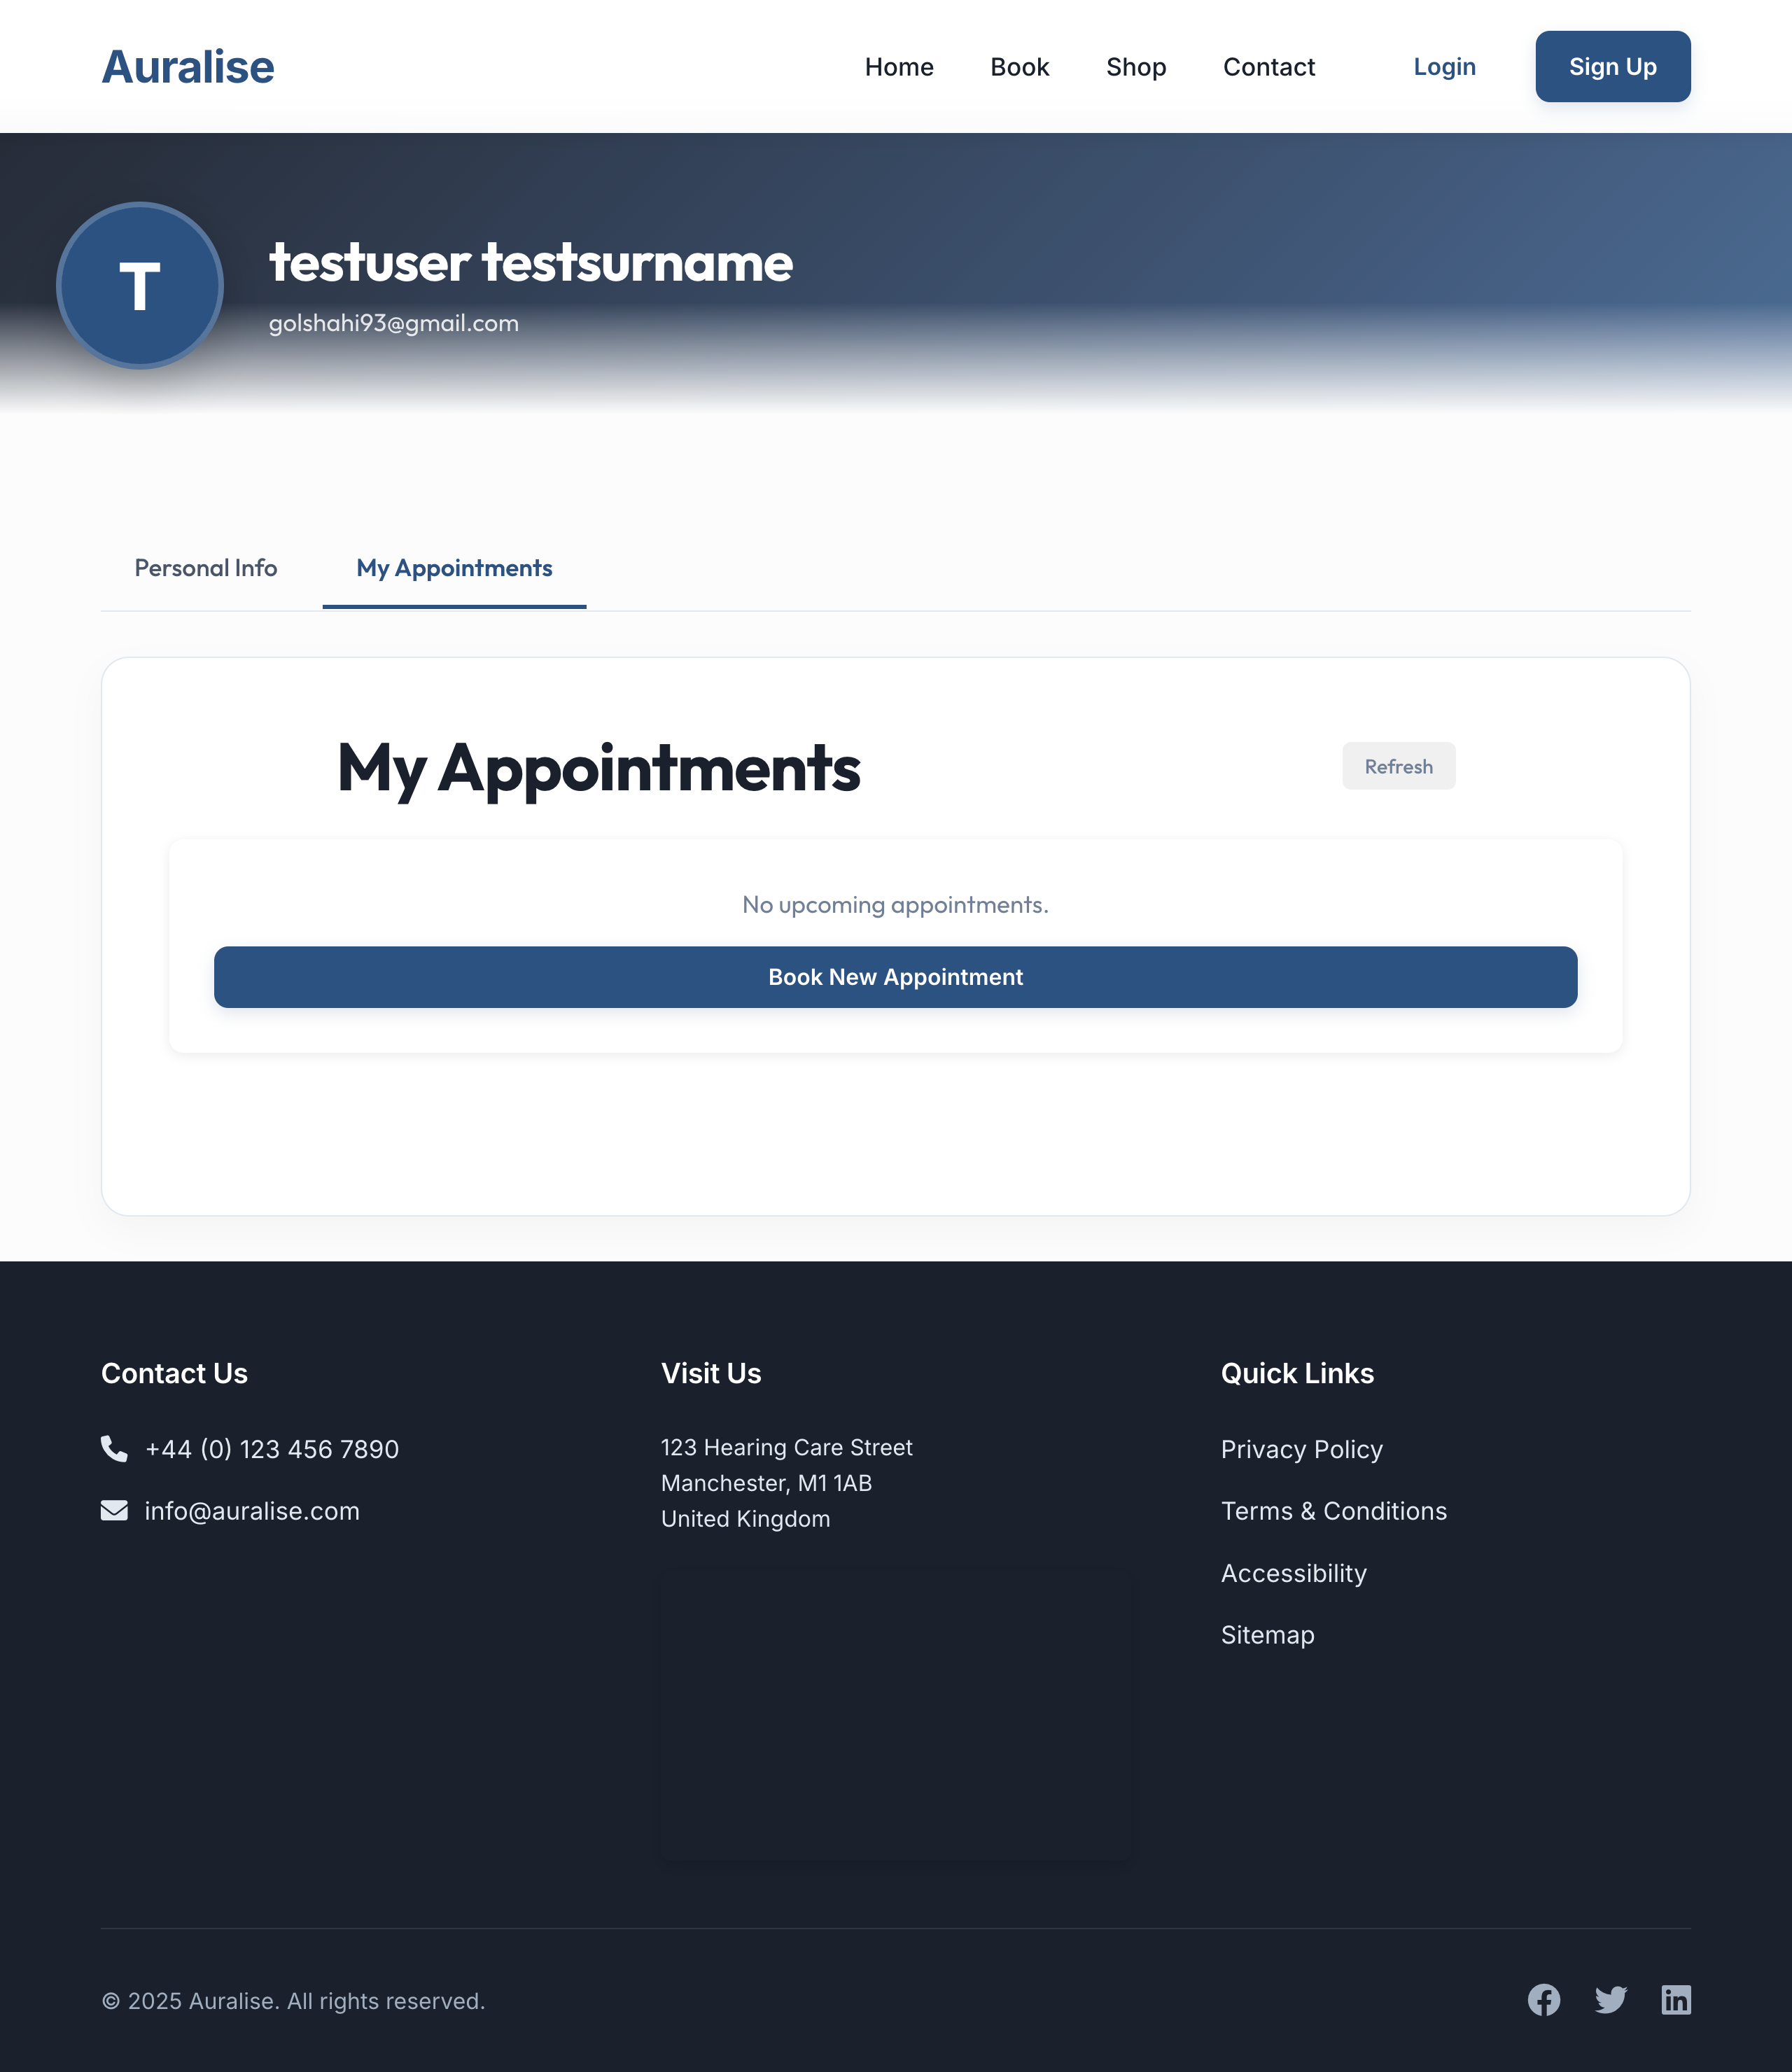
\includegraphics[height=0.3\textheight, keepaspectratio]{desktop_appointment_history.png}
    \subcaption{Desktop Appointment History}
\end{subfigure}
\caption{Appointment History (Mobile and Desktop)}
\label{fig:appointment_history}
\end{figure}


The Profile Page serves as a dashboard for the user's hearing healthcare journey. It displays personal information and provides access to:

\begin{enumerate}
    \item Personal Information: Seen in Figure~\ref{fig:user_profile_page}, it shows the settings for updating contact details, notification preferences, and account security options.
    \item Appointment History: Seen in Figure~\ref{fig:appointment_history}, it shows the records of past consultations and upcoming appointments with options to reschedule or cancel.
\end{enumerate}

\subsubsection{Accessibility Features}

The Hearing Aid Platform incorporates numerous accessibility features to ensure a positive experience for users with hearing impairments:

\begin{enumerate}
    \item Text Alternatives: All audio content includes captions or transcripts.
    \item Visual Indicators: Sound-based interactions are accompanied by visual feedback.
    \item Customizable UI: Text size and contrast can be adjusted to accommodate users with vision impairments.
    \item Screen Reader Compatibility: All interface elements are properly labeled for screen reader compatibility.
    \item Keyboard Navigation: The entire application can be navigated without requiring a mouse.
\end{enumerate}

These accessibility features not only help users with hearing loss but also demonstrate the platform's commitment to inclusive design principles that benefit all users.

\subsubsection{Progressive Web App Features}

As a Progressive Web App (PWA), the Hearing Aid Platform offers advanced features that enhance the user experience:

\begin{enumerate}
    \item Offline Access: Core content and previously viewed product information are available even without an internet connection.
    \item Home Screen Installation: Users can add the application to their device's home screen for quick access.
    \item Push Notifications: Optional alerts for appointment reminders and hearing care tips (with user permission).
    \item Fast Loading: Optimized assets ensure quick initial loading and smooth navigation between pages.
\end{enumerate}

These PWA capabilities create an app-like experience within the browser, providing convenience without requiring users to download and install a traditional mobile application.

\subsection{Code Structure}
This subsection provides an overview of the key architectural components and implementation patterns used in the Hearing Aid Platform.

\subsubsection{Frontend Architecture}
The frontend is built using React with TypeScript, following a component-based architecture. The main application router (App.tsx) defines the navigation structure and provides route protection for authenticated sections.

A simplified extract of the routing configuration is shown in Figure \ref{fig:app_tsx}. The full App.tsx source code can be found in the Appendix, Listing~\ref{fig:full_app_tsx}.

\begin{lstlisting}[language=JavaScript, caption={App.tsx - Main Application Router}, label={fig:app_tsx}]
const App: React.FC = () => {
  return (
    <Router>
      <AuthProvider>
      <ScrollToTop />
      <div className="app">
        <Header />
        <Routes>
          <Route path="/" element={<HomePage />} />
          <Route path="/book" element={<BookPage />} />
          <Route path="/contact" element={<ContactPage />} />
          <Route path="/shop" element={<ShopPage />} />
          <Route path="/shop/product/:id" element={<ProductPage />} />
          <Route path="/try-on/:productId" element={<TryOnARPage />} />
          <Route path="/hearing-test" element={<HearingTestPage />} />
          <Route path="/login" element={<LoginPage />} />
          <Route path="/signup" element={<LoginPage />} />
          <Route path="/profile" element={<ProfilePage/>}/>
          <Route path="/booking-confirmation" element={<BookingConfirmationPage/>}/>
          <Route path="/verify" element={<VerifyEmailPage/>}/>
        </Routes>
        <Footer />
      </div>
      </AuthProvider>
    </Router>
  );
};
\end{lstlisting}

\subsubsection{Component Architecture}
The application follows a modular, component-based structure, emphasizing reusability and separation of concerns. Key components are briefly described below:

\begin{itemize} 
    \item HearingAidModel: Implements 3D model rendering using React Three Fiber 
    \item ContextualHearingTest: Manages the speech understanding assessment 
    \item AudiogramGraph: Visualizes hearing test results 
    \item BookPage: Handles appointment scheduling 
\end{itemize}

A full listing of the source code for these components is provided in the Appendix, Listings \ref{fig:hearingaidmodel}--\ref{fig:bookpage}.

\subsubsection{Backend Architecture}
The backend is implemented in Kotlin using the Ktor framework, following a clean architecture pattern. The main layers are:

\begin{itemize} 
    \item Routes: Defines RESTful API endpoints, organized by resource \item Models: Data classes representing entities, including validation rules 
    \item Repositories: Manages database access, interacting with Azure Cosmos DB 
    \item Services: Implements business logic and application workflows \end{itemize}

Full code listings for representative backend modules are provided in the Appendix, Listings \ref{lst:routes}--\ref{lst:service}.

\subsubsection{Key Features Implementation}
The platform integrates several sophisticated features to enhance user experience and functionality:

\begin{itemize} 
    \item AR Try-On: Utilizes WebGL and Three.js for interactive 3D rendering of hearing aids 
    \item Hearing Test: Implements the Web Audio API for precise frequency tone generation and playback 
    \item Appointment System: Provides real-time availability checking and appointment booking 
    \item Authentication: Secures user access with JWT-based authentication and email verification 
\end{itemize}

Full code listings for the implementation of these features are provided in the Appendix, Listings \ref{lst:artryon}--\ref{lst:authentication}.

\subsubsection{Progressive Web App Features}
The application is configured as a Progressive Web App (PWA) to enhance user experience on mobile and desktop devices. Core PWA functionalities include:

\begin{itemize} 
    \item Service Worker: Enables offline functionality and background sync 
    \item App Manifest: Provides metadata for installation and homescreen access 
    \item Caching Strategies: Implements asset caching to improve load performance 
    \item Push Notifications: Supports real-time updates via browser notifications 
\end{itemize}

Full code listings related to PWA configuration and features are provided in the Appendix, Listings \ref{lst:serviceworker}--\ref{lst:appmanifest}.

\newpage


\fancyhead[L]{} 
\fancyhead[L]{\textbf{7 Testing} \vspace{1pt}} % "CONTENTS" title

\section{Testing}
Testing is a crucial aspect of web application development that ensures the reliability, functionality, and user experience of the Hearing Aid Platform \cite{geeksforgeeks_web_testing_2024}. Through systematic testing, developers can verify the application's usability, correctness, and functional behavior. This section details the testing methodologies employed, including black box testing, regression testing, and white box testing \cite{nidhra_black_2012}.

\subsection{Black Box Testing}
Black box testing was conducted based on the end-user perspective to validate the overall functionality of the system. The testing focused on the functional requirements specified in Section 5 (System Requirements). The results are presented in Tables \ref{tab:sprint1-testing}, \ref{tab:sprint2-testing}, and \ref{tab:sprint3-testing}.

\begin{table}[H]
\centering
\label{tab:sprint1-testing}
\begin{tabular}{|c|p{6cm}|c|c|}
\hline
\textbf{FR ID} & \textbf{Test Case Description} & \textbf{Priority} & \textbf{Result} \\ \hline
FR01 & Verify hearing aid listing with prices and features & \textcolor{red}{Must Have} & \textcolor{green}{Passed} \\ \hline
FR03 & Test appointment booking for all service types & \textcolor{red}{Must Have} & \textcolor{green}{Passed} \\ \hline
FR04 & Validate AI-driven hearing test functionality & \textcolor{red}{Must Have} & \textcolor{green}{Passed} \\ \hline
FR05 & Test contact form and support system & \textcolor{red}{Must Have} & \textcolor{green}{Passed} \\ \hline
\end{tabular}
\caption{Sprint 1 Black Box Testing Results}
\end{table}

\begin{table}[H]
\centering
\label{tab:sprint2-testing}
\begin{tabular}{|c|p{6cm}|c|c|}
\hline
\textbf{FR ID} & \textbf{Test Case Description} & \textbf{Priority} & \textbf{Result} \\ \hline
FR02 & Test AR functionality for hearing aid visualization & \textcolor{red}{Must Have} & \textcolor{green}{Passed} \\ \hline
FR14 & Verify audiologist appointment management & \textcolor{red}{Must Have} & \textcolor{green}{Passed} \\ \hline
FR15 & Test audiologist profile management & \textcolor{red}{Must Have} & \textcolor{green}{Passed} \\ \hline
FR06 & Validate appointment/hearing aid recommendation quiz & \textcolor{orange}{Should Have} & \textcolor{green}{Passed} \\ \hline
FR07 & Test multiple payment method integration & \textcolor{orange}{Should Have} & \textcolor{green}{Passed} \\ \hline
\end{tabular}
\caption{Sprint 2 Black Box Testing Results}
\end{table}

\begin{table}[H]
\centering
\label{tab:sprint3-testing}
\begin{tabular}{|c|p{6cm}|c|c|}
\hline
\textbf{FR ID} & \textbf{Test Case Description} & \textbf{Priority} & \textbf{Result} \\ \hline
FR16 & Test audiologist availability management & \textcolor{orange}{Should Have} & \textcolor{green}{Passed} \\ \hline
FR08 & Verify user profile management and feedback system & \textcolor{green}{Could Have} & \textcolor{green}{Passed} \\ \hline
FR09 & Test notification system functionality & \textcolor{green}{Could Have} & \textcolor{green}{Passed} \\ \hline
FR17 & Validate appointment type specification & \textcolor{green}{Could Have} & \textcolor{green}{Passed} \\ \hline
\end{tabular}
\caption{Sprint 3 Black Box Testing Results}
\end{table}

\subsubsection{Regression Testing}
Regression testing was performed throughout the development process to ensure that new changes did not affect existing functionality. This testing was conducted after each sprint and major feature implementation \cite{grjoeay_regression_2024}. The regression testing focused on:

\begin{itemize}
    \item Core functionality verification after each sprint
    \item Integration testing between frontend and backend components
    \item API endpoint consistency and reliability
    \item Database operations and data integrity
    \item User authentication and authorization flows
\end{itemize}

All regression tests passed successfully across all three sprints, confirming that new features and modifications did not break existing functionality.

\subsection{White Box Testing}
White box testing was conducted to verify the internal logic and structure of the application. The testing focused on specific components and their interactions. Table \ref{tab:whitebox-testing} presents the white box testing results.

\begin{table}[H]
\centering
\label{tab:whitebox-testing}
\begin{tabular}{|c|p{6cm}|c|}
\hline
\textbf{Component} & \textbf{Test Case Description} & \textbf{Result} \\ \hline
Authentication & User registration and login flow & \textcolor{green}{Passed} \\ \hline
Appointment System & Booking creation and management & \textcolor{green}{Passed} \\ \hline
AR Integration & 3D model loading and rendering & \textcolor{green}{Passed} \\ \hline
Notification System & Email and in-app notification delivery & \textcolor{green}{Passed} \\ \hline
Database Operations & CRUD operations and data consistency & \textcolor{green}{Passed} \\ \hline
API Endpoints & Request handling and response validation & \textcolor{green}{Passed} \\ \hline
\end{tabular}
\caption{White Box Testing Results}
\label{tab:whitebox-testing}
\end{table}

The white box testing covered critical aspects of the application, including:
\begin{itemize}
    \item Code coverage analysis
    \item API endpoint testing
    \item Database query optimization
    \item Error handling and logging
    \item Security implementation verification
    \item Performance optimization validation
\end{itemize}

All white box tests passed successfully, indicating robust internal implementation and reliable system architecture. The testing results demonstrate that the Hearing Aid Platform meets all specified requirements and maintains high standards of code quality and system reliability.

\newpage

\fancyhead[L]{} 
\fancyhead[L]{\textbf{8 Evaluation} \vspace{1pt}} % "CONTENTS" title

\section{Evaluation}
This section provides a comprehensive evaluation of the development and implementation of the Hearing Aid Platform project. It is divided into the Achievements, Final Gantt Chart, Experience, and Future Work sub-sections.

\subsection{Achievements}
The main achievement of this project was the development of a modern web-based platform that allows users to explore hearing aid options, book appointments, and complete AI-driven hearing assessments through an intuitive and accessible interface. All the functional requirements specified during the System Analysis (Section 5) were successfully met, including:

\begin{itemize}
    \item A complete hearing aid catalog with detailed features and pricing.
    \item An advanced appointment booking system for a variety of services.
    \item AI-powered hearing test functionality.
    \item AR-based hearing aid visualization.
    \item A comprehensive audiologist management system.
    \item A user profile and notification system to ensure seamless communication.
\end{itemize}

Throughout the development process, there was excellent coordination with the project supervisor, and any feedback from meetings and reviews was effectively incorporated into the platform. A strong emphasis was placed on ensuring the platform remained responsive, accessible, and user-friendly, catering to users of all technical abilities. The integration of Augmented Reality (AR) for real-time product visualization and AI technologies for hearing tests represent significant technical accomplishments in the hearing healthcare domain.
\\\\
Overall, I am very satisfied with the final outcome and believe that the project achieved all the initial goals that were set at the beginning of the implementation phase.

\subsection{Final Gantt Chart}
\begin{figure}[H]
    \centering
    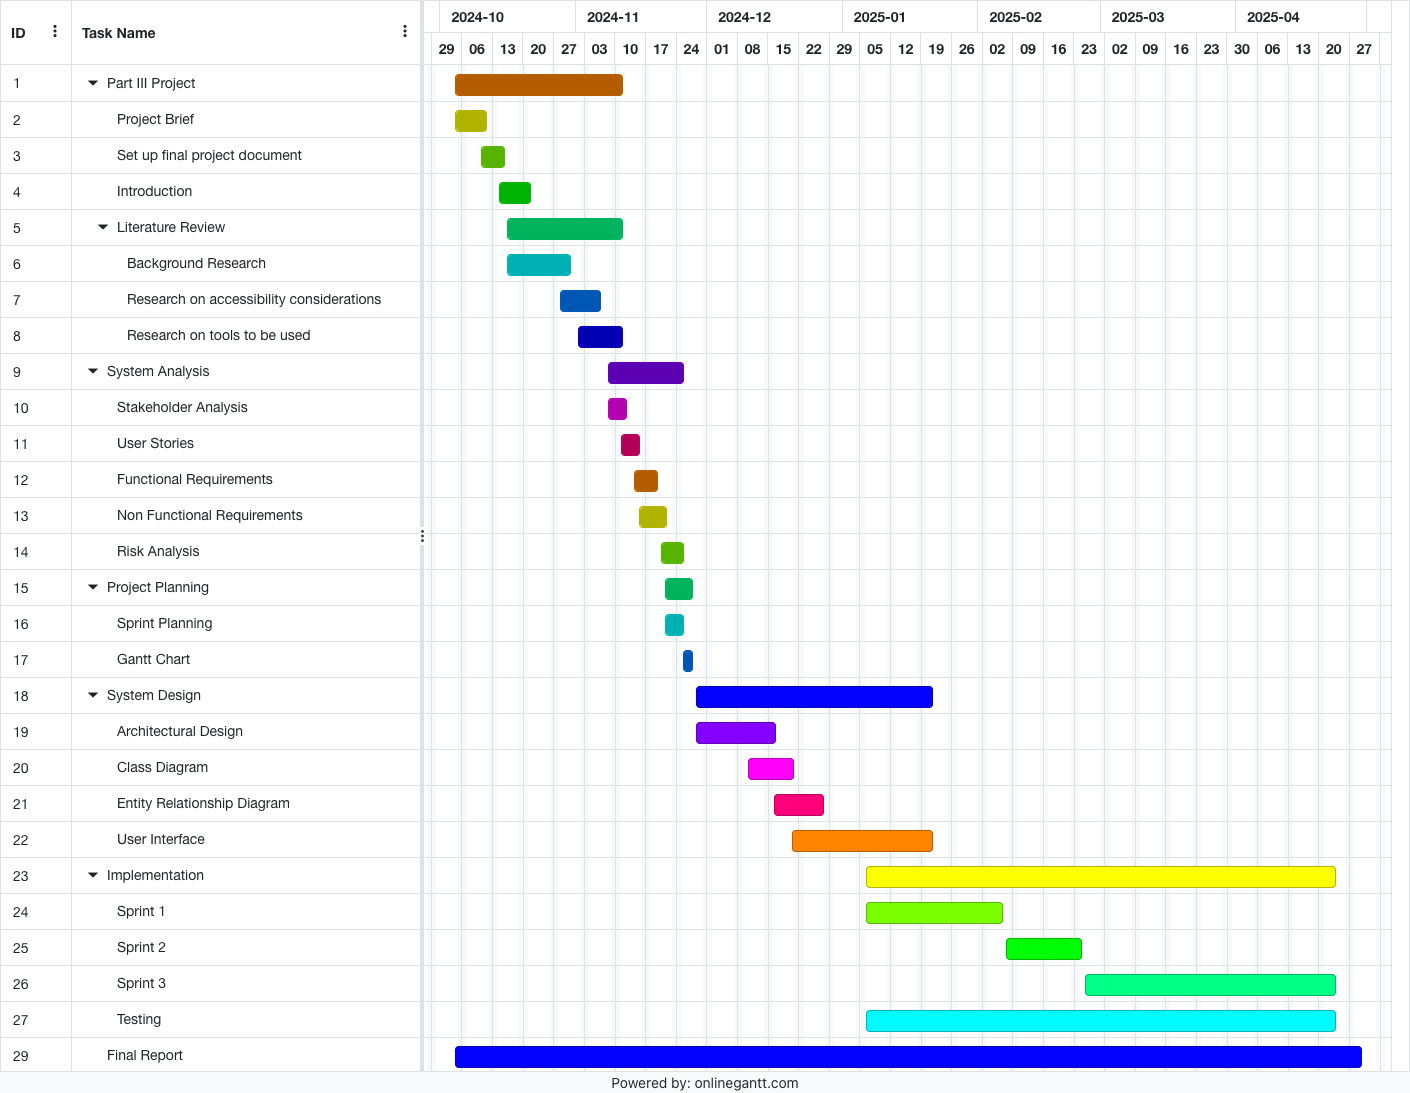
\includegraphics[width=\textwidth]{Final Gantt Chart.png}
    \caption{Actual Project timeline acheived in the Gantt Chart.}
    \label{fig:final_gantt_chart}
\end{figure}

The final Gantt Chart as shown in Figure~\ref{fig:final_gantt_chart} illustrates the real-world timeline of the project, including the three sprints and their respective deliverables. Although there were some slight adjustments compared to the original timeline due to unforeseen circumstances, all key milestones were completed within the project scope.
The three main sprints built progressively on each other, and any delays encountered were managed effectively to ensure the final deliverables were not compromised. Testing was done alongside development following a partial test driven development strategy and final polishing were completed on time, allowing the platform and the report to be ready for submission by the deadline.

\subsection{Experience}
This section reflects on the experience gained throughout the project.
\subsubsection{Development}
This project provided significant hands-on experience in full-stack web development and emerging technologies. Key areas of growth include:

\begin{itemize}
    \item Modern web development using React and TypeScript.
    \item Integrating AR technology for product visualization (using AR.js and Three.js).
    \item Implementing AI-driven hearing assessment algorithms.
    \item Building secure authentication and authorization systems.
    \item Designing and managing a cloud-based database.
    \item Developing and integrating RESTful APIs (using Node.js and Express.js).
\end{itemize}

Particularly, integrating AR and AI technologies was both challenging and rewarding. These areas required additional research and experimentation, which greatly expanded my technical capabilities and confidence in handling complex, multi-technology projects.

\subsubsection{Tools and Environments}
Several tools and environments were instrumental during the development:

\begin{itemize}
    \item \textbf{Development Environment:}
    \begin{itemize}
        \item VS Code was used for code editing.
        \item Git for version control, ensuring organized and trackable development.
        \item npm for managing dependencies.
    \end{itemize}
    
    \item \textbf{Frontend Technologies:}
    \begin{itemize}
        \item React for building responsive UIs.
        \item TypeScript for ensuring type safety and better project scalability.
        \item Three.js for rendering 3D models.
        \item AR.js for implementing AR features.
    \end{itemize}
    
    \item \textbf{Backend Technologies:}
    \begin{itemize}
        \item Node.js for server-side scripting.
        \item Express.js for creating APIs.
        \item Azure Cosmos DB for database management.
    \end{itemize}
\end{itemize}

Working with these tools not only reinforced existing skills but also introduced new techniques for professional-grade application development.

\subsubsection{Testing}
Testing was an essential part of the project, with key experiences including:

\begin{itemize}
    \item Conducting black-box testing to validate functionality from the user's perspective.
    \item Employing white-box testing for unit and component-level verification.
    \item Performing regression testing after each sprint to ensure no features were broken.
    \item Integrating frontend and backend components through thorough integration testing.
    \item Carrying out performance testing to ensure the platform's speed and reliability.
\end{itemize}

Testing throughout the development cycle ensured the system remained stable, functional, and user-friendly.

\subsection{Future Work}
While the platform successfully meets all initial objectives, there are several opportunities for future improvements:

\subsubsection{Enhanced AR Features}
\begin{itemize}
    \item Implement higher-quality 3D models for hearing aids.
    \item Allow real-time color customization during AR visualization.
    \item Improve mobile AR functionality by utilizing device cameras.
    \item Add an AR-based fitting guide to enhance user experience.
\end{itemize}

\subsubsection{AI and Machine Learning Improvements}
\begin{itemize}
    \item Further refine hearing test algorithms for even higher accuracy.
    \item Implement personalized hearing aid recommendations.
    \item Develop predictive maintenance alerts for device servicing.
    \item Automate appointment scheduling based on user availability and audiologist schedules.
\end{itemize}

\subsubsection{User Experience Enhancements}
\begin{itemize}
    \item Develop a dedicated mobile application for iOS and Android.
    \item Add enhanced accessibility features to support users with disabilities.
    \item Introduce multi-language support to broaden user reach.
    \item Further improve the notification system for real-time updates.
\end{itemize}

\subsubsection{Integration and Security}
\begin{itemize}
    \item Integrate with additional payment gateways for broader financial flexibility.
    \item Strengthen security protocols for user data protection.
    \item Explore integration with electronic health records (EHR) systems like Apple Health.    
    \item Implement automated backup and disaster recovery systems.
\end{itemize}

\subsubsection{Testing and Quality Assurance}
\begin{itemize}
    \item Introduce automated test suites for continuous integration/continuous deployment (CI/CD).
    \item Further optimize performance for faster load times.
    \item Improve error handling across the platform.
    \item Carry out comprehensive security and penetration testing.
\end{itemize}

By pursuing these improvements, the Hearing Aid Platform could evolve into an even more powerful and comprehensive solution for hearing healthcare services.

\newpage

\fancyhead[L]{} 
\fancyhead[L]{\textbf{9 Conclusion} \vspace{1pt}} % "CONTENTS" title
\section{Conclusion}
This project addresses the challenge of making hearing healthcare services more accessible and user-friendly through digital innovation. The report provides a detailed analysis of the system requirements, project planning, and system design, explaining how the Hearing Aid Platform was carefully planned and, based on these sections, successfully developed and tested.
\\\\
It is clear that the Hearing Aid Platform has achieved all of its primary goals and milestones that were set during the initial project planning. The platform enables users to explore and purchase hearing aids through an intuitive interface, provides accurate AI-driven hearing assessments, and enhances user experience with real-time Augmented Reality visualization. Furthermore, the appointment booking system and audiologist management features ensure streamlined communication and service delivery between patients and healthcare providers. The user profile and notification systems have also been implemented successfully, ensuring smooth interactions throughout the platform.
\\\\
Through this project, valuable experience was gained in full-stack web development, AR technology, and healthcare system integration. The platform has proven that modern technologies such as Augmented Reality and Artificial Intelligence can be effectively incorporated into healthcare services, creating a strong foundation for future improvements. Overall, the successful completion of this project represents a significant step towards modernizing and improving accessibility to hearing healthcare services.



















\end{document}
